%
% Tesi D.S.I. - modello preso da
% Stanford University PhD thesis style -- modifications to the report style
%
%%%%%%%%%%%%%%%%%%%%%%%%%%%%%%%%%%%%%%%%%%%%%%%%%%%%%%%%%%%%%%%%%%%%%%%%%%%
%                                                                         %
%			TESI DOTTORATO                                                   %
%			______________                                                   %
%                                                                         %
%			AUTORE: Elena Pagani                                             %
%                                                                         %
%			Ultima revisione: 7.X.1998                                       %
%                                                                         %
%%%%%%%%%%%%%%%%%%%%%%%%%%%%%%%%%%%%%%%%%%%%%%%%%%%%%%%%%%%%%%%%%%%%%%%%%%%
%
%
\documentclass[12pt]{report}
%    \renewcommand{\baselinestretch}{1.6}      % interline spacing
%
% \includeonly{}
%
%			PREAMBOLO
%
\usepackage[a4paper]{geometry}
\usepackage{amssymb,amsmath,amsthm}
\usepackage{csvsimple}
\usepackage{graphicx}
\usepackage{mathtools}
\usepackage{amsthm}
\usepackage{url}
\usepackage{hyperref}
\usepackage{epsfig}
\usepackage[italian]{babel}
\usepackage{listings}
\usepackage{color}
\usepackage{relsize}
\usepackage{pgfplotstable,filecontents}
\usepackage{algorithm}
\usepackage[noend]{algpseudocode}
\usepackage[toc,page]{appendix}
\usepackage{longtable}
\usepackage{subcaption}
\makeatletter
\renewcommand*{\ALG@name}{Pseudocodice}
\makeatother

\newtheorem{theo}{Teorema}

\definecolor{codegreen}{rgb}{0,0.6,0}
\definecolor{codegray}{rgb}{0.5,0.5,0.5}
\definecolor{codepurple}{rgb}{0.58,0,0.82}
\definecolor{backcolour}{rgb}{0.95,0.95,0.92}
\lstdefinestyle{mystyle}{
    backgroundcolor=\color{backcolour},   
    commentstyle=\color{codegreen},
    keywordstyle=\color{blue},
    numberstyle=\tiny\color{codegray},
    stringstyle=\color{codepurple},
    basicstyle=\footnotesize,
    breakatwhitespace=false,         
    breaklines=true,                 
    captionpos=b,                    
    keepspaces=true,                 
    numbers=left,                    
    numbersep=5pt,                  
    showspaces=false,                
    showstringspaces=false,
    showtabs=false,                  
    tabsize=2,
    framexleftmargin=1pt
}

\lstset{style=mystyle}

% per le accentate
\usepackage[utf8]{inputenc}
%
\newtheorem{myteor}{Teorema}[section]
%
\newenvironment{teor}{\begin{myteor}\sl}{\end{myteor}}
%
%
%			TITOLO
%
\begin{document}


\begin{titlepage}
  \begin{center}
    
\includegraphics[height=5.0cm]{./images/minerva_2013_DI.jpg}
    
    \vspace*{.4cm}
    {\Large 
      \emph{Corso di Laurea Magistrale in\\[.3cm]
        Scienze e Tecnologie dell'Informazione}
      %\emph{Corso di Laurea Magistrale in Sicurezza Informatica}
      %\emph{Corso di Laurea in Informatica}
      % \emph{Corso di Laurea in\\[.3cm]
      %   Sicurezza dei Sistemi e delle Reti Informatiche}
      % \emph{Corso di Laurea in\\[.3cm]
      %   Tecnologie per la Società dell'Informazione}
    }
    \vfill
    \begin{LARGE}
      \textbf{Metodi di Ensemble Gerarchici \\[.2cm] per la Predizione Strutturata \\[.3cm]della Funzione delle Proteine}
    \end{LARGE}
    
    \vfill
    \begin{minipage}{.99\linewidth}
      \begin{tabular}{l r}
        \begin{minipage}{.4\linewidth}
          \begin{flushleft}
            {\large
              RELATORE\\[.3cm]
              Prof. Giorgio Valentini
            }

            % \vspace*{1.5cm}
            {\large
              CORRELATORE\\[.3cm]
               Dr. Marco NOTARO
            }
          \end{flushleft}
        \end{minipage}
        &
        \begin{minipage}{.6\linewidth}
          \begin{flushright}
            {\large
              TESI DI LAUREA DI\\[.3cm]
              Marco ODORE\\[.45cm]
              Matr. 868906
            }
          \end{flushright}
        \end{minipage}
      \end{tabular}
    \end{minipage}
    
    \vfill
    {\large{{Anno Accademico 2017/2018}}}
  \end{center}
\end{titlepage}

%
%
%			ORGANIZZAZIONE
%TO DO
%
%			RINGRAZIAMENTI
%
%\prefacesection{Ringraziamenti}

%\afterpreface
% 
% 

\Large
 \begin{center}
\textbf{ABSTRACT}
\end{center}

\hspace{10pt}

% Author names and affiliations


\normalsize

Il problema della predizione della funzione delle proteine \`e uno dei problemi centrali della Biologia Computazionale e presenta diversi problemi aperti sia da un punto visto computazionale sia da un punto di vista biologico.

Uno dei problemi rilevanti in questo ambito \`e rappresentato dal fatto che ad ogni proteina possono essere associate funzioni molteplici e tali funzioni possono essere rappresentate tramite classe funzionali (termini) a loro volta strutturate secondo un grafo diretto aciclico (DAG). Dal punto di vista dell'apprendimento automatico questo problema pu\`o essere modellato con un problema di classificazione multi-label strutturato, in cui le predizioni associate ad ogni proteina sono insiemi di termini della Gene Ontology (GO) strutturate secondo un DAG.

Recentemente sono stati proposti diversi metodi di ensemble gerarchici, progettati proprio per la predizione stutturata dei termini della Gene Ontology (e pi\`u in generale per tassonomie organizzate secondo un DAG). Tali metodi si caratterizzano per procedure di learning a due passi, caratterizzate da un primo passo di ``flat learning'' in cui le classi della GO sono apprese in modo indipendente, e da un secondo passo in cui le predizioni flat sono combinate opportunamente tramite un metodo di ensemble gerarchico.

L'obiettivo primario della tesi  consiste nel confrontare metodi di machine learning flat con i metodi di ensemble gerarchici, in modo da valutare se ed in quali condizioni tali metodi possono migliorare significativamente le predizioni flat. 
Tale confronto  \`e effettuato utilizzando le proteine di un piccolo verme nematode, \emph{Caenorhabditis Elegans}, un organismo modello molto usato per studi di biologia dello sviluppo, il cui genoma  \`e costituito da circa 20000 geni.
I risultati mostrano che i metodi gerarchici sono in grado di migliorare sistematicamente le performance di classificazione ottenuti con un ampio spettro di metodi di apprendimento automatico e suggeriscono che tali metodi, sfruttando la loro modularit\`a, potrebbereo essere utilizzati per migliorare le prestazioni di qualsiasi algoritmo di apprendimento flat, a condizione che le predizioni flat su cui si basano gli algoritmi gerarchici non siano quasi totalmente casuali.

Nella tesi viene inoltre proposto un nuovo algoritmo di apprendimento gerarchico basato sulla isotonic regression, chiamato \emph{True Path Rule con Isotonic Regression} (ISO-TPR),
basato sull'applicazione dell'algoritmo \emph{Generalized Pool Adjacent Violators} (GPAV) nella fase ``top-down'' di apprendimento dell' algoritmo di ensemble gerarchico \emph{True Path Rule}. I risultati ottenuti con tale metodo sono risultati essere competitivi con i metodi di ensemble gerarchici allo stato dell'arte per la predizione della funzione delle proteine.

La tesi \`e suddivisa in diverse sezioni:

\begin{itemize}
\item Una parte introduttiva, in cui sono affrontate le criticit\`a e caratteristiche del problema della predizione della funzione delle proteine (capitolo 1). 
\item Una parte metodologica, in cui si analizzano i metodi ensemble utilizzati allo stato dell'arte, e le nuove proposte (GPAV e ISO-TPR) (capitolo 2).
\item Una parte di analisi preliminare del problema specifico di classificazione (Predizione della funzione delle proteine per la specie \emph{C. Elegans}), in cui viene descritto il dataset utilizzato, gli algoritmi di machine learning utilizzati per implementare i base learner dei metodi ensemble, le metriche di valutazione, le stime dei tempi di calcolo, e i metodi per la riduzione della complessit\`a temporale risultante da un problema di classificaione strutturata con migliaia di classi. (Capitolo 3, fino al paragrafo 3.6).
\item Una parte sperimentale di classificazione delle classi GO di \emph{C. Elegans}, in cui sono comparati ed applicati i metodi di machine learning flat ed i metodi di ensemble gerarchici su tutto il dataset, valutandone i risultati in relazione a metriche ``per-classe''  e ``per-proteina''. (Capitolo 3, dal paragrafo 3.6 fino al 3.9).
\item Una parte conclusiva in cui si riassumono i risultati ottenuti, evidenziando in che misura e quando i metodi ensemble sono risultati efficaci e proponendo eventuali lavori futuri. (Capitolo 4).
\end{itemize}
\tableofcontents


%			CAPITOLO 1: dshjkfg
\chapter{Il problema della predizione della funzione delle proteine tramite metodi automatici}

La predizione della funzione delle proteine costituisce uno dei problemi fondamentali nell'ambito della \emph{biologia computazionale}\cite{JIANG}. Oltre ad essere di importanza fondamentale nell'ambito della \emph{biologia molecolare}, costituisce inoltre un  problema rilevante anche per la \emph{medicina genomica}\cite{LEUNG}.
\newline
\newline
La classificazione delle proteine effettuata in maniera \emph{automatica}\cite{gfp}, nasce dall'esigenza di gestire la grossa mole di nuovi dati genomici e proteomici non categorizzati, che oggi giorno risulta essere in continua crescita. A causa di questo incremento, l'etichettatura manuale  risulta infatti estremamente costosa in termini di tempo e risorse diventando di fatto impraticabile.
\newline
\newline
Nel caso specifico della predizione della funzione delle proteine\footnote{\footnotesize{All'interno della tesi la parole \emph{gene} verrà utilizzata in maniera intercambiale con la parola \emph{proteina}, dato che associare una funzione (o più funzioni) ad una proteina, equivale ad associare la stessa al gene che la codifica.}}, vi sono due tassonomie principali che relazionano le diverse classi\footnote{\footnotesize{All'interno della tesi, le parole \emph{classe}, \emph{annotazione}, \emph{funzione} e \emph{termine} verranno utilizzate in maniera intercambiabile, volendo identificare lo stesso concetto.}}:

\begin{enumerate}
\item La \emph{Gene Ontology} (GO)\cite{go}: Definisce l'universo di concetti in relazione alle funzioni dei geni e alla loro localizzazione nella cellula.
\item Il \emph{Functional Catalogue} (FunCat)\cite{FunCat}: Definisce uno schema alternativo e più sintetico per la classificazione funzionale delle proteine.
\end{enumerate}

La GO presenta una granularità fine, mentre quella di FunCat è più grossolana, ma la principale differenza è nel modo in cui sono messe in relazione le classi all'interno delle rispettive gerarchie. La GO è infatti strutturata come un \emph{grafo diretto aciclico} (DAG), e ogni singolo arco indica diversi tipi di relazione tra le classi\cite{GO:REL}, e cioè:
\begin{itemize}
\item\emph{is a}: relazione di sotto-tipo.
\item \emph{a part of}: relazione di composizione
\item \emph{regulates}: relazione di influenza/regolazione
\end{itemize} 

Mentre FunCat è organizzato come un \emph{albero}\footnote{\footnotesize{Sia il DAG che l'albero sono grafi, ma il DAG è un grafo diretto aciclico, dove un nodo può avere più genitori, a differenza dell'albero in cui ogni nodo ha al più un genitore.}}. Degli esempi di DAG per la GO e albero per FunCat sono mostrati nella figura \ref{DAGTREE}.
\newline
\newline
\begin{figure}[h]
\center
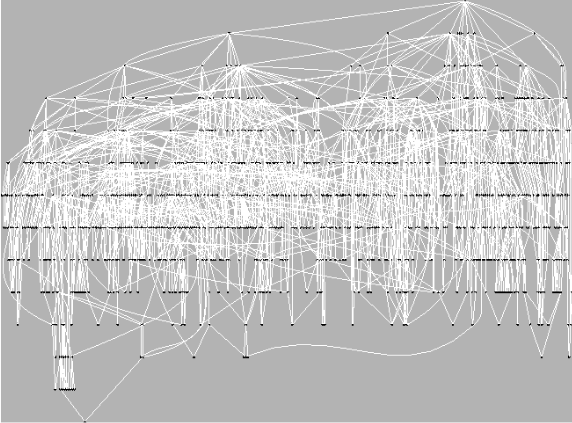
\includegraphics[scale=0.3]{./images/GO.png}
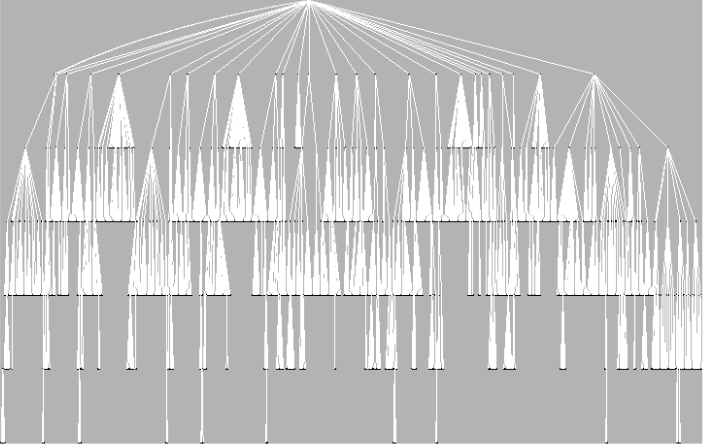
\includegraphics[scale=0.29]{./images/FunCat.png}
\caption{\footnotesize{A sinistra un DAG della GO per la specie \emph{S. cerevisiae}. A destra FunCat.}}
\label{DAGTREE}
\end{figure}
\newline
\newline
Inoltre la GO presenta una caratterizzazione ulteriore, poiché viene suddivisa in 3 diverse ontologie:
\begin{itemize}
\item \textit{Biological Process:} descrive i processi ad alto livello, come insieme di diverse attività molecolari.
\item \emph{Molecular Function:}                  descrive le funzioni di specifici prodotti genici.
\item \emph{Cellular Component:} il luogo all'interno della cellula (nello specifico le strutture cellulari) nelle quali avviene la funzione genica.
\end{itemize}

FunCat possiede un albero fisso, con 1362 categorie funzionali, suddivise su 6 livelli di diversa specificità. È comparabile alle classi delle ontologie Molecular Function e Biological Process della GO.
\newline
\newline
Le annotazioni dei geni per FunCat e la GO sono governate dalla \emph{True Path Rule} (anche conosciuta come \emph{annotation propagation rule})\cite{TOPDOWN}, una regola che garantisce la consistenza delle annotazioni. Se un gene è annotato con un determinato termine (funzione) della GO o di FunCat, allora risulta annotato anche per i predecessori (avi e genitori) di tale termine, in maniera ricorsiva. Al contrario, se un gene non è annotato per un termine, non può esserlo per i discendenti di quest'ultimo. Nella figura \ref{tpr_ex} sono mostrati alcuni esempi esplicativi sulla True Path Rule.
\newline
\begin{figure}[h]
\center
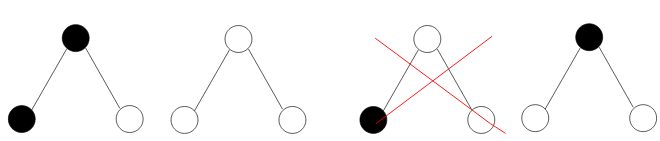
\includegraphics[scale=0.55]{./images/tpr_rule.png}
\caption{\footnotesize{Esempi che mostrano come viene applicata la True Path Rule. I nodi in nero indicano l'annotazione, quelli in bianco l'assenza di annotazione. Il primo, il secondo e l'ultimo esempio risultano essere consistenti, mentre il terzo no. In quanto il gene risulta essere annotato per un termine, ma non per il suo genitore.}}
\label{tpr_ex}
\end{figure}
\newline
Data la granularità e specificità superiori della GO e il suo largo utilizzo nella comunità scientifica, all'interno della tesi ci si è soffermati sulla predizione delle sue funzioni.
\newline
\newline
In letteratura sono noti diversi metodi per la predizione della funzione delle proteine\cite{valentiniMethods}, che possiamo raggruppare in quattro macro categorie:
\begin{enumerate}
\item Metodi basati sulla \emph{biosequenza}.
\item Metodi basati su \emph{reti}.
\item Metodi \emph{kernel per spazi di output strutturati}.
\item Metodi \emph{ensemble gerarchici}.
\end{enumerate}
\section{Metodi basati sulla comparazione di biosequenze}
I metodi basati sull'allineamento di biosequenze\footnote{\footnotesize{Esistono diversi tipi di sequenze, ad esempio quelle degli amminoacidi o dei nucleotidi.}} rappresentano un primo tentativo di predirre computazionalmente la funzione delle proteine. L'idea di questa tecnica si basa sul fatto che sequenze simili condividano funzioni comuni.
\newline
\newline
Esistono diversi metodi ed euristiche per la ricerca di biosequenze simile. Degli esempi sono ad esempio gli algoritmi euristici \emph{FASTA}\cite{Fasta} e \emph{BLAST}\cite{Blast}.  
\section{Metodi basati su reti}

Questi metodi sono applicati a dati rappresentati sotto forma di grafo non direzionato $G = (V, E)$, dove i nodi $v \in V$ corrispondono ai geni e i lati $e \in E$ sono pesati in relazione al grado di co-funzionalità specificata dalla sorgente dati.
\newline
\newline
Tramite delle \emph{relazioni di prossimità} tra i nodi connessi, questi metodi sono capaci di trasferire annotazioni da nodi precedentemente annotati a quelli che non lo sono. 
\newline
\newline
Esistono diversi \emph{algoritmi di propagazione delle etichette}(o annotazioni), come ad esempio:
\begin{itemize}
\item Metodi che valutano il flusso funzionale dei grafi. \cite{flow}
\item Metodi semi-supervisionati come le reti di \emph{HopField}\cite{hopfield}.
\item Metodi basati su \emph{Markov} \cite{markov}.
\item Metodi basati sui \emph{Campi Gaussiani Aleatori} \cite{campigauss}.
\item Metodi \emph{Guilty-by-association} \cite{guilty}.
\item Metodi basati su funzioni obiettivo con kernel. \cite{kernelVal}
\end{itemize} 
\section{Metodi Kernel per spazi di output strutturati}
I metodi \emph{kernel} sono metodi molto utilizzati per problemi di classificazione. Tramite una mappatura \emph{non lineare} dello spazio di partenza delle feature è infatti possibile ottenere un predittore non lineare, sfruttando algoritmi nati per la separazione lineare. L'idea base è quella di sfruttare quindi un predittore lineare, del tipo:
\[
f(x) = w^T \phi(x)
\]
Dove $x$ rappresenta il vettore istanza in input, e $w$ è un vettore di pesi. $\phi$ è la funzione di mapping, che trasforma lo spazio di partenza $R^d$\footnote{\footnote{Dove $d$ è il numero di feature dello spazio di partenza.}}, in un nuovo spazio $R^k$, con $k>>d$
\[
\phi : R^d \rightarrow R^k.
\]

Dato poi che il vettore $w$, ottenuto dall'apprendimento di algoritmi come il \emph{percettrone}\cite{PERC}, può essere rappresentato come una somma pesata del tipo:
\[
w = \sum_{i \in S} y_i \phi(x_i)
\]
dove $S$ è l'insieme delle istanze di training e le $y_i$ sono le etichette, possiamo trasformare il predittore come
\[
f(x) = \sum_{i\in S} y_i \phi(x_i)^T \phi(x)
\]
L'idea del metodo consiste infine di rendere computazionalmente gestibile il prodotto $\phi(x_i)^T \phi(x)$, sostituendolo con una funzione kernel:
\[
\phi(x_i)^T \phi(x) = K(x_i, x)
\]
trasformando quindi il predittore lineare in una funzione del tipo:
\[
f(x) = \sum_{i \in S} y_i K(x_i, x)
\]
La criticità di questo approccio è che risulta non applicabile a problemi con output strutturato, come nel caso del problema della predizione della funzione delle proteine. Per ovviare a questa situazione, si può utilizzare una funzione kernel congiunta del tipo:
\[
K : (x \times y) \times (x \times y) \rightarrow R
\]
che tiene conto sia degli input ($x$) che degli output ($y$), computando la compatibilità di una data coppia di input-output. Il predittore finale si occuperà infine di selezionare l'etichetta con la maggior compatibilità.
\newline
\newline
Esempi di metodi di questo tipo sono:
\begin{itemize}
\item \emph{Percettrone strutturato} \cite{perceptron}
\item Algoritmi di \emph{margine massimo} per output strutturati \cite{marginemassimo}
\end{itemize}
\section{Metodi ensemble gerarchici}
Sono metodi che tengono in considerazione esplicitamente le relazioni gerarchiche tra i termini funzionali. Sono definiti metodi \emph{ensemble}\footnote{\footnotesize{Gli ensemble di classificatori sono insiemi di predittori che lavorano assieme per risolvere un problema di classificazione.}} perché vengono addestrati indipendentemente diversi predittori (uno per classe funzionale della gerarchia), le cui predizioni vengono poi \emph{combinate} in una seconda fase. Questa fase, definita di ensemble o di correzione, si rende necessaria in quanto ogni predittore non è a conoscenza della struttura gerarchica dell'output (essendo addestrato indipendentemente) e può quindi generare risultati errati e inconsistenti rispetto alla gerarchia delle classi. Un esempio generale di ensemble di predittori, lo troviamo in figura \ref{ensembleex}.
\begin{figure}[h]
\centering
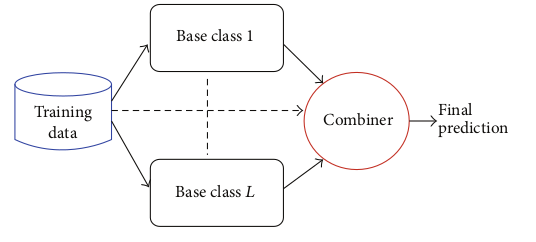
\includegraphics[scale=0.6]{./images/ensemble.png}
\caption{\footnotesize{Schema generale di un metodo di ensemble. L diversi classificatori base (Base Class) sono addestrati e le loro predizioni sono combinate per ottenere una predizione "consensus" dell'ensemble.}}
\label{ensembleex}
\end{figure}
\newline
\newline
Esistono diversi tipi di metodi ensemble gerarchici, ad esempio:
\begin{itemize}
\item Metodi \emph{Top-Down} \cite{TOPDOWN}
\item Metodi \emph{Bayesiani}\cite{BAYESIAN}
\item Metodi di \emph{Riconciliazione} \cite{reconcil}
\item Metodi basati sulla \emph{True Path Rule} \cite{TOPDOWN}
\item Metodi basati sugli \emph{alberi di decisione} \cite{decisionTree}
\end{itemize}

In questa tesi ci si è soffermati allo studio di alcuni metodi di Ensemble Gerarchici (Top-Down e  basati sulla True Path Rule).
\chapter{Metodi di ensemble gerarchici per predizioni strutturate}
I \emph{Metodi di Ensemble Gerarchici}\cite{valentiniMethods}  sono metodi caratterizzati da due step principali:
\begin{enumerate}
\item Predizione flat delle diverse classi dell'ontologia, in maniera indipendente.
\item Combinazione e correzione delle predizioni sfruttando la relazione gerarchica tra i termini della GO.
\end{enumerate}
Il secondo step rappresenta la componente \emph{ensemble} del metodo, in quanto sfrutta gli score ottenuti dai diversi predittori generati in fase di learning, modificandoli e tendendo in considerazione la struttura dell'output. Questo permette di migliorare l'accuratezza e di rendere consistenti le predizioni fatte precedentemente. Un esempio in cui vengono mostrate le due fasi dei metodi ensemble gerarchici, lo troviamo in figura \ref{exhierarchical}.
\begin{figure}[h]
\centering
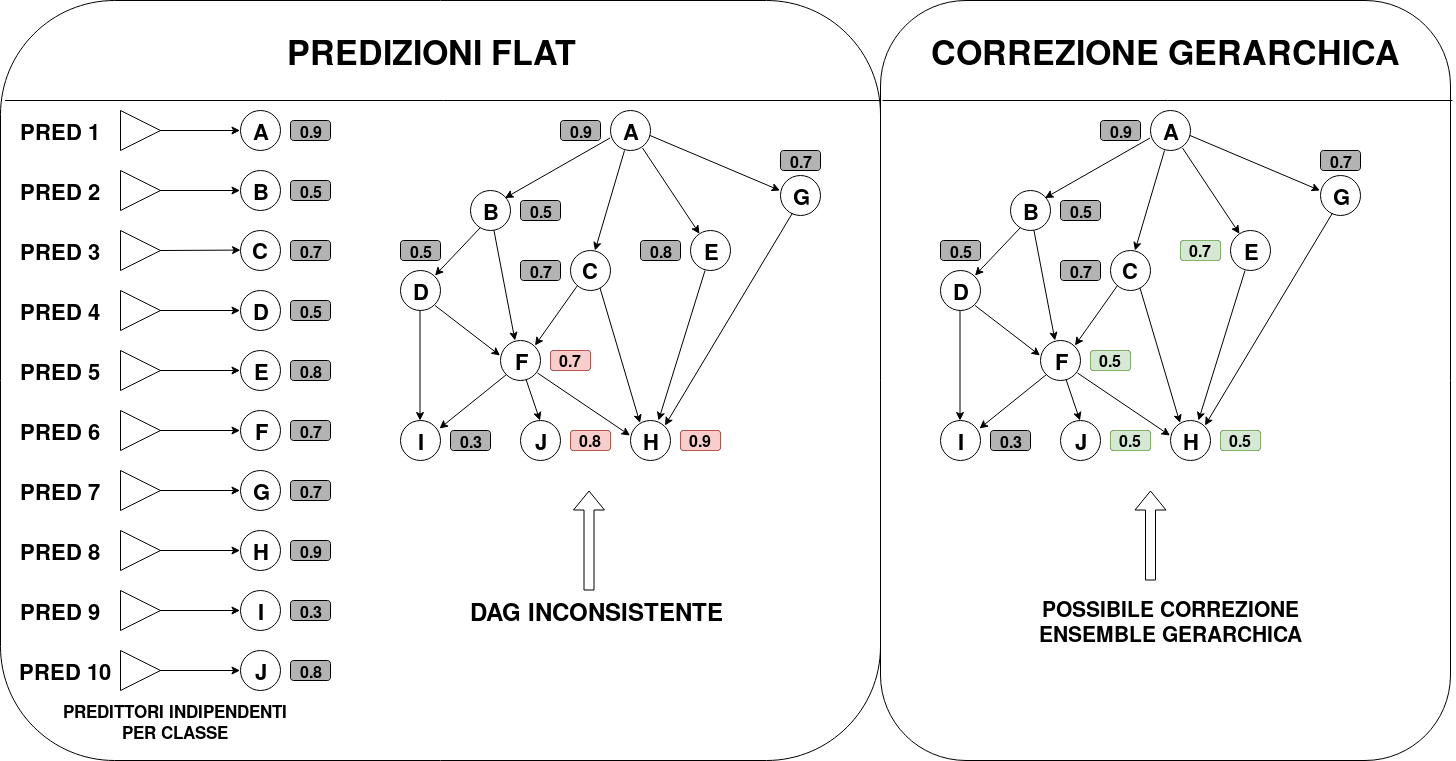
\includegraphics[scale=0.29]{./images/exensemble.png}
\caption{\footnotesize{Esempio in cui vengono mostrati i due step dei metodi ensemble gerarchici. Nel primo step vengono generati gli score flat, che per alcuni nodi/termini risultano inconsistenti (F, J, H), secondo la \emph{True Path Rule}, che verrà spiegata nel dettaglio in seguito. Nello step gerarchico ensemble vengono corretti alcuni score in modo da rendere il risultato globale consistente.}}
\label{exhierarchical}
\end{figure}

\section{Predizione flat}
La predizione \textit{flat} consiste nel trattare ogni annotazione del grafo come un problema di classificazione indipendente e slegato dagli altri termini. Questa tipologia di predizione non tiene quindi in considerazione la struttura dell'ontologia su cui viene applicata. 
\newline
\newline
Questo porta ad avere delle predizioni \emph{inconsistenti} (che non rispettano la \emph{True Path Rule}), ma portando un vantaggio in termini di semplicità e applicazione.
\newline
\newline
\newpage

\textbf{Consistenza \& True Path Rule}

Un insieme di predizioni $\hat{y} = <\hat{y}_1, \hat{y}_2, \dots, \hat{y}_{|N|}>$, dove $|N|$ è la cardinalità dei termini della gerarchia, è definito \emph{consistente}, se rispetta la \emph{True Path Rule}, e cioè:
\[
y\;\;\;consistente\;\; \leftrightarrow \forall i \in N, j \in par(i) \rightarrow y_j \geq y_i
\] 
Dove $par(i)$ indica l'insieme dei termini genitori del nodo $i$ nella gerarchia.
\newline
\newline
Essendo i problemi slegati dal grafo e gestiti indipendentemente, questi possono essere trattati con diversi algoritmi di apprendimento automatico, scegliendo in base alla situazione e necessità i metodi più idonei.

\section{Metodi ensemble}
Tra le diverse tecniche ensemble utilizzate per la correzione delle predizioni flat, in questa tesi descriviamo quelle che sfruttano l'approccio \emph{Top Down} e la \emph{True Path Rule}. Per quest'ultima verrà descritto un nuovo metodo, che implementa in modo efficiente la \emph{isotonic regression} per il passo top-down dell'algoritmo True Path Rule per DAG.
\subsection{Metodo Top-Down gerarchico (HTD-DAG)}
L'approccio Top-Down\cite{notaro1} consiste nel modificare le predizioni base dei predittori dall'alto verso il basso, e cioè dalle classi più generali a quelle più specifiche.
\newline
\newline
La correzione avviene ricorsivamente, percorrendo il grafo per \emph{livelli}. Più precisamente, dato il grafo $G = (N, E)$, gli score flat $f(x) = \hat{y}$ sono corretti gerarchicamente a $\bar{y}$, applicando la seguente regola:
\[
\bar{y}_i := 
\begin{cases}
\hat{y}_i \;\;\;\;\;\;\;\;\;\;\;\;\;\;\;\;\;\;\;\;\; if\;\; i \in root(G)\\
min_{j \in par(i)} \bar{y}_j \;\;\;\; if \;\; min_{j \in par(i)}\bar{y}_j < \hat{y}_i\\
\hat{y}_i \;\;\;\;\;\;\;\;\;\;\;\;\;\;\;\;\;\;\;\;\; altrimenti
\end{cases}
\]
Dove $par(i)$ specifica i genitori del nodo $i$.
\newline
\newline
Per garantire la correttezza e consistenza delle correzioni, i \emph{livelli} del grafo sono definiti come \emph{cammino massimo dalla radice}. Più formalmente, dobbiamo definire una funzione $\psi$ che, applicata ad un nodo $i \in N$, restituisce il livello associato al cammino massimo, cioè:
\[
\psi(i) = max_{p(i, r)}\; l(p(r, i))
\]
dove la funzione $p(r, i)$ calcola il cammino dalla radice $r$ al nodo $i$ e la funzione $l$ restituisce il livello associato ad un cammino.
\newline
Come algoritmi per il calcolo del cammino massimo si possono utilizzare ad esempio quello di \emph{Bellman-Ford} o i metodi basati sull'ordinamento topologico\cite{BELLMAN}.
\newline
\newline
Nello pseudocodice \ref{HTDDAG} è mostrato il funzionamento dell'algoritmo HTD-DAG.
\begin{algorithm}[!htp]
\begin{algorithmic}[1]
\State \textbf{Input: }
\State $G = (N, E)$
\State $N = \{1, 2, ..., |N|\} $ 
\State $\hat{y} = <\hat{y}_1, \hat{y}_2, ...,\hat{y}_{|N|}>$
\Procedure{HTD-DAG}{}
\State dist := \textbf{computeMaxDistances}(G)
\State // \textbf{Correzione Top-Down}
\State $\bar{y}_r := \hat{y}_r$  // nodo radice 
\For{each $d$ from 1 to max(dist)}
\State $N_d := \{i|dist(i) = d\}$ // nodi a distanza $d$ 
\For{each $i \in N_{d}$}
\State $x:= min_{j \in par(i)} \bar{y}$
\If {$x < \hat{y}_i$}
\State $\bar{y}_i := x $
\Else
\State $\bar{y}_i := \hat{y}_i $
\EndIf
\EndFor
\EndFor
\EndProcedure
\State \textbf{Output: }
\State $\bar{y} = <\bar{y}_1, \bar{y}_2, ...,\bar{y}_{|N|}>$
\end{algorithmic}
\caption{HTD-DAG}
\label{HTDDAG}
\end{algorithm}

La consistenza delle predizioni per il metodo HTD-DAG è dimostrata dal teorema \ref{theo1}\footnote{\footnotesize{Per la dimostrazione del teorema si rimanda al paper \cite{notaro1}}}.
\begin{theo}
Dato un grafo diretto aciclico $G = (N, E)$, la funzione $\psi$ che assegna a un nodo il suo livello in relazione al suo cammino massimo dalla radice, e l'insieme delle predizioni  $\hat{y} = <\hat{y}_1, \hat{y}_2, \dots, \hat{y}_{|N|}>$, la correzione dell'algoritmo HTD-DAG assicura che il set di predizioni ensemble $\bar{y} = <\bar{y}_1, \bar{y}_2, \dots, \bar{y}_{|N|}>$ soddisfi la seguente proprietà: $\forall i \in N, j \in par(i) \rightarrow y_j \geq y_i$.
\label{theo1}
\end{theo}
\subsection{Metodo True Path Rule (TPR-DAG)}
La correzione basata sulla True Path Rule\cite{notaro1}, integra la correzione HTD, introducendo uno step ulteriore, e cioè quello che corregge le predizioni flat dalle classi più specifiche a quelle più generali, in maniera quindi \emph{bottom-up}. Lo step top-down è invece effettuato alla stessa maniera del metodo HTD. 
\newline
\newline
Lo step bottom-up permette di trasferire informazione dalle predizioni che sono considerate \emph{positive}. Più specificatamente, data una predizione $\hat{y}_{i}$ per il nodo $i \in N$, questa può essere aggiornata come:
\[
\bar{y}_i = \frac{1}{1 + |\phi_i|} (\hat{y}_i + \sum_{j \in \phi_i} \bar{y}_j)
\]
Dove $\phi_i$ rappresenta l'insieme dei figli del nodo $i$ che sono considerati \emph{positivi} in relazione alla predizione.
In tal senso, esistono diverse strategie per la selezione dei figli positivi di un nodo $i$, come ad esempio:
\begin{itemize}
\item Selezione con soglia costante: la predizione viene considerata positiva se supera una soglia.
\item Selezione con soglia adattiva: la soglia è selezionata per massimizzare una metrica. 
\item Selezione priva di soglia: vengono considerati positivi quei nodi che incrementano il valore della predizione del genitore.
\end{itemize}
A seguito dello step bottom-up, deve poi essere eseguito lo step top-down della strategia HTD, in quanto la propagazione delle predizioni positive dal basso verso l'alto non garantisce la \emph{consistenza} delle predizioni necessarie alla TPR. Nello pseudocodice \ref{tpr-dag-code} sono specificati tutti i passaggi del metodo TPR-DAG.

\begin{algorithm}[!htp]
\begin{algorithmic}[1]
\State \textbf{Input: }
\State $G = (N, E)$
\State $N = \{1, 2, ..., |N|\} $ 
\State $\hat{y} = <\hat{y}_1, \hat{y}_2, ...,\hat{y}_{|N|}>$
\Procedure{TPR-DAG}{}
\State dist := \textbf{computeMaxDistances}(G)
\State // \textbf{Step Bottom-Up}
\For{each $d$ from max(dist) to 0}
\State $N_d := \{i|dist(i) = d\}$ // nodi a distanza $d$ 
\For{each $i \in N_{d}$}
\State $\phi_i :=$  \textbf{getPositiveChildren}(i) // seleziona i figli con un metodo
\State $\bar{y}_i = \frac{1}{1 + |\phi_i|} (\hat{y}_i + \sum_{j \in \phi_i} \bar{y}_j)$
\EndFor
\EndFor
\State $\hat{y} = \bar{y}$
\State // \textbf{Step Top-Down}
\State $\bar{y}_r := \hat{y}_r$  // nodo radice 
\For{each $d$ from 1 to max(dist)}
\State $N_d := \{i|dist(i) = d\}$ // nodi a distanza $d$ 
\For{each $i \in N_{d}$}
\State $x:= min_{j \in par(i)} \bar{y}$
\If {$x < \hat{y}_i$}
\State $\bar{y}_i := x $
\Else
\State $\bar{y}_i := \hat{y}_i $
\EndIf
\EndFor
\EndFor
\EndProcedure
\State \textbf{Output: }
\State $\bar{y} = <\bar{y}_1, \bar{y}_2, ...,\bar{y}_{|N|}>$
\end{algorithmic}
\caption{TPR-DAG}
\label{tpr-dag-code}
\end{algorithm}

Per l'algoritmo TPR-DAG valgono i seguenti teoremi\footnote{\footnotesize{Per la dimostrazione dei teoremi si rimanda al paper \cite{notaro1}}}:

\begin{theo}
Dato un grafo diretto aciclico $G = (N, E)$ e l'insieme delle predizioni flat $\hat{y} = <\hat{y}_1, \hat{y}_2, \dots, \hat{y}_{|N|}>$, la correzione dell'algoritmo TPR-DAG assicura che il set di predizioni ensemble $\bar{y} = <\bar{y}_1, \bar{y}_2, \dots, \bar{y}_{|N|}>$ soddisfi la seguente proprietà: $\forall i \in N, j \in anc(i) \rightarrow y_j \geq y_i$, dove $anc(i)$ è l'insieme di tutti i predecessori del nodo $i$ nella gerarchia (compresi i genitori).
\label{theo2}
\end{theo}

\begin{theo}
L'algoritmo ensemble TPR-DAG con la selezione dei positivi $\phi_i$, tale che $\phi_i := \{j \in child(i)|\bar{y}_j > \hat{y}_i\}$, ottiene sempre una Recall\footnote{\footnotesize{Per i dettagli della metrica si rimanda al capitolo 3.4.}} uguale o maggiore dell'algoritmo ensemble HTD-DAG.
\label{theo3}
\end{theo}
Non è garantita invece che la \emph{Precision}\footnote{\footnotesize{Per i dettagli della metrica si rimanda al capitolo 3.4.}}  dell'algoritmo TPR-DAG sia sempre migliore o uguale a quella dell'algoritmo HTD-DAG.
\subsection{Metodo True Path Rule con Isotonic Regression (ISO-TPR)}
Per il passo Top-Down dell'algoritmo TPR-DAG è possibile sfruttare gli algoritmi per la risoluzione dei problemi di \emph{Isotonic Regression} (IR) (chiamati anche di \emph{Monotonic Regression}). In questa sezione discuteremo di uno di questi metodi, noto \emph{come Pool-Adjacent-Violators}, capace di risolvere il problema in maniera efficiente.

\subsubsection{Pool-Adjacent-Violators (PAV)}
L'algoritmo PAV è utilizzato per la risoluzione dei problemi di IR, in cui si esegue il fitting di una linea (senza vincolo di forma) ad una sequenza di osservazioni, rispettando dei vincoli di \emph{ordinamento totale}. Questi vincoli fanno in modo cioè che i punti della linea, output della regressione, siano crescenti. Più formalmente, PAV risolve problemi di minimo del tipo:
\[
\min_x \sum_{i=1}^{n} w_i (x_i - a_i)^2
\]
\begin{center}
such that $x_1 \le x_2 \le ... \le x_n$ 
\end{center}
Dove le $a_i$, sono le nostre $n$ osservazioni e le $x_i$ i valori ricercati. I valori $w_i$ sono degli eventuali pesi associati all'equazione (generalmente settati a 1).
\newline
\newline
Un esempio di isotonic regression con ordinamento totale messo a confronto con una regressione lineare\cite{wikimonotonic}, lo troviamo nella figura \ref{isotonic}.
\begin{figure}[h]
\centering
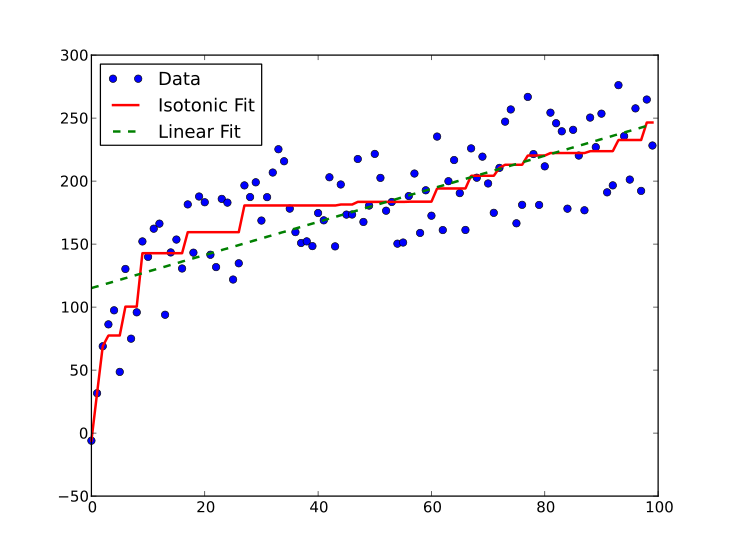
\includegraphics[scale=0.35]{./images/monotonic.png}
\caption{\footnotesize{Un esempio di IR (linea rossa)  a confronto con una regressione lineare (linea tratteggiata).}}
\label{isotonic}
\end{figure}
\newline
\newline
Essendo un problema quadratico (quindi convesso), la soluzione è unica. Per la sua risoluzione, PAV ha una complessità computazionale pari a $O(n)$. 

\subsubsection{Generalizzazione dell'algoritmo PAV (GPAV)}
Generalizzando la isotonic regression, e cioè non avendo necessariamente un vincolo di ordinamento totale, il problema può essere riformulato sotto forma di grafo aciclico diretto (DAG). Più formalmente, dato un DAG, $G(N, E)$, con il set di nodi $N = \{1, 2, ..., n\}$, si deve trovare il vettore $x^{*}\in R^{n}$ tale che:
\[
min \sum_{i=1}^{n} w_i (x_i - a_i)^2
\]
\begin{center}
such that $x_i \le x_j$ $\forall (i,j) \in E $ 
\end{center}
Dove diciamo che $x_i$ è \emph{adiacente} alla componente $x_j$ se $(i, j)\in E$.
\newline
\newline
Tale problema è risolvibile dalla versione generalizzata di PAV (GPAV) con un complessità computazionale pari a $O(n^2)$\cite{GPAV}.
\newline
\newline
L'algoritmo GPAV genera uno split del set di nodi $N$, in blocchi disgiunti. Il valore dei nodi all'interno di questi blocchi è il medesimo e per questa motivazione ognuno dei blocchi è rappresentato da un singolo elemento, chiamato \emph{head}. Formalizzando, il blocco rappresentato dal nodo (head) $i\in N$, viene denotato dal simbolo $B_i$. Il set di blocchi è invece rappresentato dall'insieme $H$, per cui valgono le seguenti proprietà:
\[
H  \subseteq N,\;\; \forall i \in H
\]
\[
\cup_{i\in H}B_i = N
\]
\[
B_i \cap B_j = 0, \;\; \forall i,j \in H,
\]
Ogni componente di $x$, associato ad un blocco $B_i \in H$, ha il medesimo valore, calcolato come segue:
\[
x_j = \frac{\sum_{k \in B_{i}} w_k a_k }{W_i}, \;\; \forall j \in B_i
\]
Dove $W_i$, peso del blocco $B_i$, è calcolato come:
\[
W_i = \sum_{k \in B_i} w_k
\]
Per il caso specifico in cui $w_k = 1, \forall k \in B_i$, si ottiene 
\[
x_j = \frac{\sum_{k\in B_i} a_k}{|B_i|}
\]
Dove $|B_i|$ è la cardinalità del blocco $B_i$.
\newline
\newline
Dato poi un nodo $i\in N$, l'insieme dei suoi  predecessori immediati $j$, e cioè, tali che, $\{j \in N :(j, i) \in E\} $, viene denotato con $i^{-}$. Il blocco $B_i$  è detto \emph{adiacente} al blocco $B_j$, o immediato predecessore, se esiste un $k \in B_i $ e un $l \in B_j$ tali che $k \in l^{-}$. Sia infine $B_i^{-}$ il set di nodi immediatamente adiacenti a $B_i$. 
\newline
\newline
L'algoritmo GPAV assegna nella fase iniziale $B_i = \{i\}$ e $B_i^{-} = i^{-}, \;\; \forall i \in N$. Successivamente tali blocchi si possono ridurre, in quanto un blocco ne può \emph{assorbire} uno adiacente se questo rispetta determinate condizioni.  Nello pseudocodice \ref{ABSORB} sono specificati i passaggi per la procedura di assorbimento di un blocco $B_i$ da parte di un blocco $B_j$.
\begin{algorithm}[!htp]
\caption{Absorb}\label{ABSORB}
\begin{algorithmic}[1]
\Procedure{Absorb($j, i$)}{}
\State $ H = H \backslash \{i\} $
\State $ B_j^{-} = B_i^{-}\cup B_j^{-}\backslash \{i\} $
\State $x_j = \frac{W_j x_j + W_i x_i}{W_j + W_i}$
\State $B_j = B_j \cup B_i$
\State $W_j = W_j + W_i$
\For{(each $k \in H\;\; s.t.\;\; i  \in B_k^{-} $)}
\State $B_k^{-} = B_k^{-}\backslash \{i\} \cup \{j\}$ 
\EndFor
\EndProcedure
\end{algorithmic}
\end{algorithm}
\newpage
Assumendo che i nodi siano stati pre ordinati topologicamente\footnote{\footnotesize{Esiste una soluzione esatta per determinati ordinamenti topologici del grafo\cite{optimGPAV}.}}, GPAV esegue le operazioni specificate nello pseudocodice \ref{gpav}

\begin{algorithm}[!htp]
\caption{GPAV}\label{gpav}
\begin{algorithmic}[1]
\State \textbf{Input: }
\State $G = (N, E)$
\State $N = \{1, 2, ..., |N|\} $ 
\State $\hat{y} = <\hat{y}_1, \hat{y}_2, ...,\hat{y}_{|N|}>$
\Procedure{GPAV}{}
\State $ H = N $
\For{(each $i \in N$)}
\State $B_i = \{i\}$ 
\State $B_i^{-} = i^{-}$
\State $x_i = \hat{y}_i$
\State $W_i = w_i$
\EndFor
\For{$k = 1, 2, ..., n$}
\State \emph{// finché esiste un predecessore di $B_{k}$ che viola la monotonicità}
\While{$\{i \in B_k^{-}: x_i \geq x_k\}\neq 0$} 
\State \emph{// Trova l'elemento che viola maggiormente il vincolo}
\State \textbf{Find} $j \in B_k: U_j = max\{U_i : i \in B_k^{-}\}$ 
\State \textbf{Absorb(i, j)} \emph{// $j$ viene assorbito da $B_i$}
\EndWhile
\EndFor
\State \emph{//Aggiornamento per soluzione finale }  
\For{each $k \in H$}
\For{each $i \in B_k$}
\State $\bar{y}_i = x_i$  
\EndFor
\EndFor
\EndProcedure
\State \textbf{Output: }
\State $\bar{y} = <\bar{y}_1, \bar{y}_2, ...,\bar{y}_{|N|}>$
\end{algorithmic}
\end{algorithm}

Riassumendo, l'algoritmo effettua degli assorbimenti di blocchi adiacenti, finché questi violano i vincoli del problema quadratico, generando di fatto una partizione dei nodi, in cui le parti condividono lo stesso valore.

\subsubsection{ISO-TPR}
Sostituendo quindi il secondo step del metodo TPR-DAG, e cioè quello top down, con GPAV, otteniamo l'algoritmo ISO-TPR. Lo schema di tale algoritmo è riassunto nello pseudocodice \ref{ISOTPR}.

\begin{algorithm}[!htp]

\begin{algorithmic}[1]
\State \textbf{Input: }
\State $G = (N, E)$
\State $N = \{1, 2, ..., |N|\} $ 
\State $\hat{y} = <\hat{y}_1, \hat{y}_2, ...,\hat{y}_{|N|}>$
\Procedure{ISO-TPR}{}
\State dist := \textbf{computeMaxDistances}(G)
\State // \textbf{Step Bottom-Up}
\For{each $d$ from max(dist) to 0}
\State $N_d := \{i|dist(i) = d\}$ // nodi a distanza $d$ 
\For{each $i \in N_{d}$}
\State $\phi_i :=$  \textbf{getPositiveChildren}(i) // seleziona i figli con un metodo
\State $\bar{y}_i = \frac{1}{1 + |\phi_i|} (\hat{y}_i + \sum_{j \in \phi_i} \bar{y}_j)$
\EndFor
\EndFor
\State $\hat{y} = \bar{y}$
\State // \textbf{Step Top-Down}
\State $ H = N $
\For{(each $i \in N$)}
\State $B_i = \{i\}$ 
\State $B_i^{-} = i^{-}$
\State $x_i = \hat{y}_i$
\State $W_i = w_i$
\EndFor
\For{$k = 1, 2, ..., n$}
\State \emph{// finché esiste un predecessore di $B_{k}$ che viola la monotonicità}
\While{$\{i \in B_k^{-}: x_i \geq x_k\}\neq 0$} 
\State \emph{// Trova l'elemento che viola maggiormente il vincolo}
\State \textbf{Find} $j \in B_k: U_j = max\{U_i : i \in B_k^{-}\}$ 
\State \textbf{Absorb(i, j)} \emph{// $j$ viene assorbito da $B_i$}
\EndWhile
\EndFor
\State \emph{//Aggiornamento per soluzione finale }  
\For{each $k \in H$}
\For{each $i \in B_k$}
\State $\bar{y}_i = x_i$  
\EndFor
\EndFor
\EndProcedure
\State \textbf{Output: }
\State $\bar{y} = <\bar{y}_1, \bar{y}_2, ...,\bar{y}_{|N|}>$
\end{algorithmic}
\caption{ISO-TPR}
\label{ISOTPR}
\end{algorithm}



\chapter{Predizione della funzione delle proteine della specie C.elegans}
Per questa tesi sono stati eseguiti degli esperimenti al fine di verificare empiricamente, tramite un problema reale di classificazione delle proteine, se ed in quali circostanze le predizioni flat possono essere migliorate da metodi di ensemble gerarchici. Nello specifico si è eseguito la sperimentazione sul genoma della specie \textit{Caenorhabditis elegans}, un organismo modello molto semplice, utilizzato frequentemente in biologia, soprattutto per studi di biologia dello sviluppo\cite{hodgkin}.
\newline
\newline


\section{Dataset}
L'insieme delle istanze utilizzato come input dai diversi algoritmi di apprendimento automatico per il nostro problema, è dato dall'insieme dei geni della specie oggetto della sperimentazione, il quale è rappresentato da una matrice simmetrica generata dal network di interazione \emph{proteina-proteina} estratto dal database \emph{STRING} (Search Tool for the Retrieval of Interacting Genes/Proteins)\footnote{\footnotesize{La versione del network di interazioni proteina-proteina è la v10.5 del 20 Dicembre 2017.}}\cite{STRING}. Le interazioni tra le proteine aiutano a descrivere e a identificare le loro funzioni: ad esempio, la struttura tridimensionale di una proteina acquisisce significato solo nel contesto di una più grande combinazione di proteine. Il database STRING integra diversi tipi \emph{canali di evidenza}\footnote{\footnotesize{\url{https://string-db.org/help/getting_started/\# evidence}}} proteina-proteina, in base alla specie di riferimento. Un network di esempio è dato dalla figura \ref{string-net}.
\begin{figure}[h]
\center
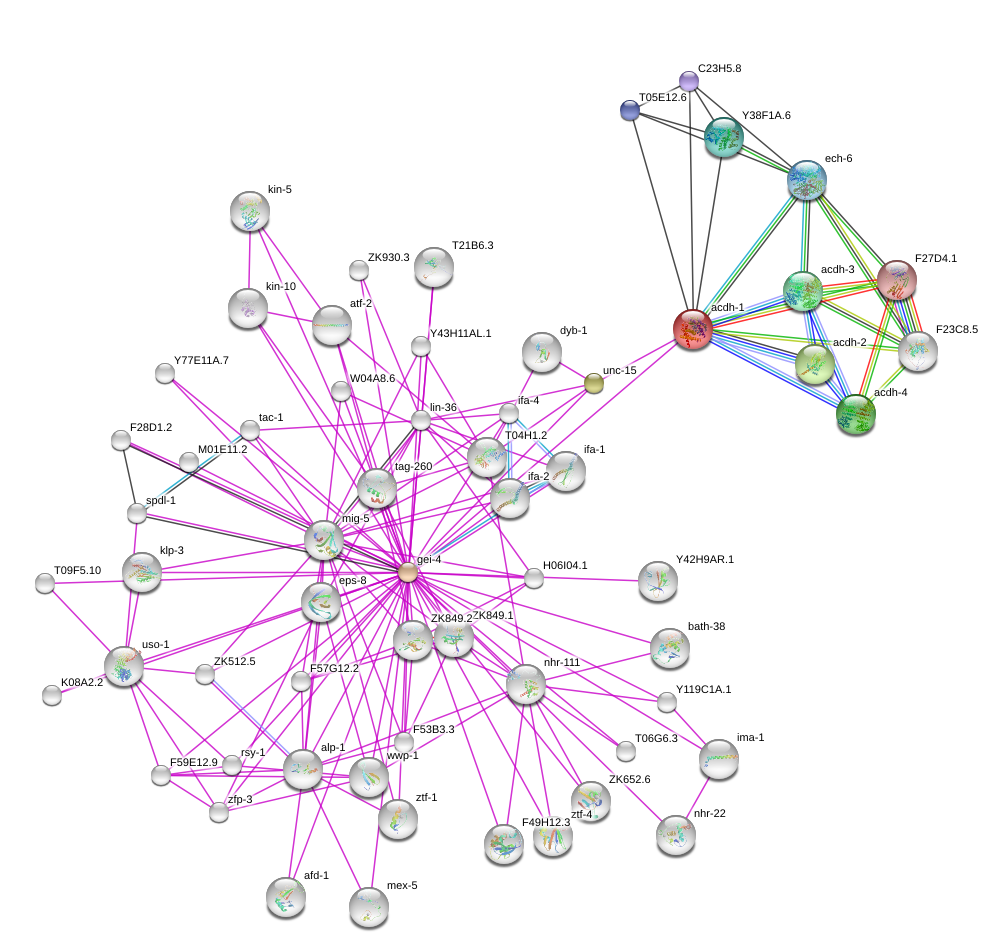
\includegraphics[scale=0.45]{./images/STRING-NET.png}
\caption{\footnotesize{Una porzione del network proteina-proteina per la specie C.elegans. I nodi rappresentano le proteine, e gli archi colorati le differenti relazioni tra queste.}}
\label{string-net}
\end{figure}
\newline
\newline
Nel caso della nostra matrice, il valore della relazione proteina-proteina è dato da uno score combinato\footnote{\footnotesize{\url{https://string-db.org/help/faq/\# how-are-the-scores-computed}}} di differenti sorgenti, e cioè:
\begin{itemize}
\item Le interazioni proteiche verificate sperimentalmente, presenti in database primari.
\item Le informazioni del pathway\footnote{\footnotesize{La via metabolica (spesso chiamata pathway metabolico o più semplicemente pathway) è l'insieme delle reazioni chimiche coinvolte in uno o più processi di anabolismo o catabolismo all'interno di una cellula.}} ottenute da database curati. 
\item I collegamenti semantici e/o statistici fra le proteine, ottenuti dall'analisi effettuata tramite text-mining di sommari MedLine e da grosse collezioni documentali. 
\item Le interazioni ottenute tramite diversi algoritmi sulle informazioni genetiche.
\item Le interazioni dei geni ortologhi, e cioè geni che sono presenti in specie diverse ma correlate, che codificano per proteine con strutture e funzioni simili.
\end{itemize} 

Questi score combinati proteina-proteina rappresentano di fatto le \emph{feature} (o \emph{caratteristiche}) delle istanze, e sono espressi con un valore intero in $[0, 1000]$, dove 1000 indica il massimo livello interazione e 0 la sua assenza. 
\newline
\newline
Nel caso specifico della specie C.elegans, la matrice STRING ha dimensione $15752 \times 15752$. 
\section{Classi/Annotazioni}
Il numero di classi per la specie C.elegans, varia di molto in base all'ontologia di riferimento della GO. Il numero delle classi (termini) aventi almeno 1 annotazione sperimentale per una proteina di C. Elegans ed i relativi archi, sono mostrati nella tabella \ref{DAG_desc}.

\begin{table}[h]
\centering
\begin{tabular}{|l|l|l|}
\hline
       ontologia & numero di termini & numero di archi \\ \hline
BP & 4068  &  8066   \\ 
\hline
MF  & 1163  & 1567   \\ 
\hline
CC  & 578  & 1082     \\ 
\hline
\end{tabular}
\caption{\footnotesize{Statistiche relative ai DAG delle annotazioni della specie C.elegans.}}
\label{DAG_desc}
\end{table}

Come si può vedere dalla precedente tabella, l'ontologia più problematica e onerosa risulta essere la BP, che oltre ad avere un numero considerevole di classi, possiede un DAG molto più complesso rispetto alle altre due gerarchie. 
\newline
\newline
\newline
Al fine di garantire che nella cross-validation non vengano generati fold privi di esempi annotati, in fase sperimentale sono state selezionate solo quelle classi che hanno almeno 10 annotazioni tra le istanze. Nella tabella \ref{riduzioneann} sono mostrate il numero di classi per ontologia, a seguito della riduzione, con annesse alcune statistiche.
\begin{table}[h]
\centering
\begin{tabular}{|l|l|l|l|l|l|}
\hline
\textbf{Onto} & \textbf{numero di termini} & \textbf{media} & \textbf{d.std.} & \textbf{massimo} & \textbf{minimo} \\ \hline
BP            & 1335                & 71,33                & 151,68              & 2597                & 10                  \\ \hline
MF            & 186                 & 61,23                & 191,84              & 1806                & 10                  \\ \hline
CC            & 221                 & 131,9                & 302,25              & 1924                & 10                  \\ \hline
\end{tabular}
\caption{\footnotesize{La colonna \emph{numero di termini} indica il numero di termini ottenuti dopo la selezione, \emph{media} la media delle annotazioni per classe, per l'ontologia di riferimento, \emph{d.std.} la deviazione standard delle annotazioni per l'ontologia di riferimento, \emph{massimo} e \emph{minimo} rispettivamente il massimo e minimo numero di annotazioni.}}
\label{riduzioneann}
\end{table}
\newpage
\section{Algoritmi di apprendimento automatico utilizzati per le predizioni flat}
Per quanto riguarda gli algoritmi di apprendmento automatico da utilizzare per le predizioni flat, si sono considerati i seguenti metodi:
\begin{enumerate}
\item \emph{K-Nearest Neighbors}\cite{KNN}
\item \emph{Logit Boost}\cite{LogitBoost}
\item \emph{Linear Discriminant Analysis}\cite{LDA}
\item \emph{eXtreme Gradient Boosting} \cite{xgbLinear}
\item \emph{C5.0} (Alberi di decisione)\cite{C5.0}
\item \emph{Random Forest}\cite{Ranger}
\item \emph{Multilayer Perceptron}\cite{mlp}
\item \emph{Support Vector Machine lineare}\cite{SVM}
\item \emph{Bagged CART} (Bagged ensemble di alberi di decisione) \cite{treebag}
\item \emph{AdaBoost.M1}\cite{adaboost}
\item \emph{Naive Bayes}\cite{naivebayes}
\item \emph{Glmnet}\cite{glmnet}
\end{enumerate}

Dato l'elevato numero di algoritmi selezionati per la sperimentazione, si è deciso di non effettuare il tuning dei parametri, questo per evitare di allungare ulteriorimente i tempi dell'intero processo di valutazione e generazione degli score flat.
\newline
\newline
Per ogni metodo si sono utilizzati valori prefissati dei parametri degli algoritmi di apprendimento. Tali valori sono riassunti nello script \ref{configs} in appendice.
\newline
\newline
Per quanto riguarda l'implementazione degli algoritmi di apprendimento si è utilizzato il package \emph{Caret}\cite{CARET} di R. In appendice è presente uno script (\ref{exampleTrainR}) di esempio di training e test dei metodi flat con cross-validation. 
\newline
\newline
Tutti i test e l'intera sperimentazione sono stati eseguiti su una macchina che dispone di:
\begin{itemize}
\item 12 Processori Intel(R) Xeon(R) CPU E5-2630 v2 @ 2.60GHz.
\item 128 GB di Memoria RAM.
\end{itemize}

\section{Valutazione delle performance}
Come metriche relative alla valutazione della qualità dei predittori sono state utilizzate due tipologie di metriche:

\begin{itemize}
\item Basate sui termini/classi. 
\item Basate sui geni.
\end{itemize} 

Per le metriche basate sui termini, si sono utilizzate l'\textit{Area Under Precision Recall Curve} (AUPRC) e l'\textit{Area Under Receiver Operating Characteristic Curve} (AUROC). 
\newline
\newline
La AUROC è una misura di \emph{robustezza} del classificatore, e mette in relazione le misure di \emph{Recall} e \emph{False Positive Rate}(FPR), al variare di una \emph{soglia} applicata all'output del modello\footnote{\footnotesize{La soglia funge da discriminante per l'output del predittore e ci permette di decidere se classificare l'istanza come appartenente alla classe di riferimento o meno. Ex. if \emph{output}$>=$soglia then 1 else 0.}}. La Recall è calcolata come:
\[
Recall = \frac{TruePositive}{TruePositive+FalseNegative}
\]
mentre la FPR come:
\[
FPR = \frac{FalsePositive}{TrueNegative+FalsePositive}
\]
Entrambe sono definite in $[0,1]$. La Recall ci indica quanti elementi sono stati classificati correttamente come \emph{rilevanti} ($TruePositive$), appartenenti cioè alla classe che si sta osservando, sul totale delle istanze appartenenti alla classe ($TruePositive+FalseNegative$). La FPR invece ci da una stima della frequenza (\emph{rate}) di istanze che sbagliamo a classificare come appartenenti alla classe ($FalsePositive$) sul totale delle istanze non appartenenti alla classe ($FalsePositive+TrueNegative$).
Facendo un plot dei valori di queste metriche al variare della soglia è possibile generare una curva, la cui area sottesa rappresenta la misura ricercata. Più il valore di quest'area si avvicina a 1, più il classificatore è considerato affidabile. Al contrario, più il risultato è vicino a $0.5$ più il predittore è vicino ad un predittore casuale.\footnote{\footnotesize{Valori vicini a $0.5$ indicano che il predittore non è tanto diverso da un predittore ottenuto con il lancio di una moneta, che predice ad esempio positivo con testa, negativo con croce. È quindi da considerarsi simile ad un predittore casuale.}}.
Un esempio di plot per i risultati di un predittore sono mostrati nella figura \ref{roc_plot_ex}.
\begin{figure}[h]
\center
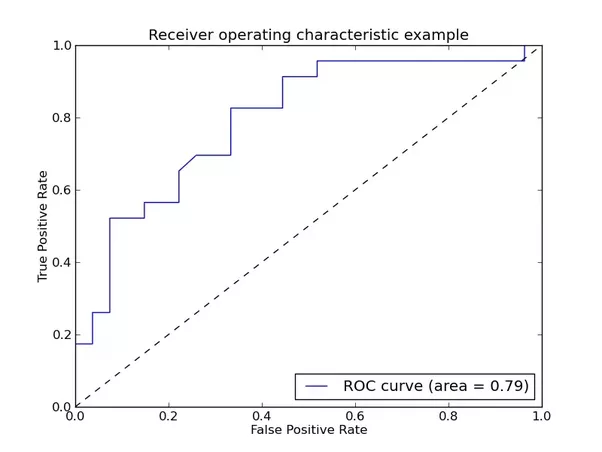
\includegraphics[scale=0.38]{./images/Roccurves.png}
\caption{\footnotesize{Un grafico generato dai diversi valori di Recall (True Positive Rate) e di False Positive Rate.}}
\label{roc_plot_ex}
\end{figure}
\newline
\newline
La metrica di AUPRC si rende invece necessaria in quanto il problema della predizione della funzione delle proteine risulta generalmente \emph{sbilanciato}. Per problemi sbilanciati ci ri riferisce a quei problemi che presentano un numero di istanze annotate di molto inferiore al numero di quelle che non lo sono. La AUPRC mette in relazione la variazione di \emph{Precision} al variare della \emph{Recall}. La Precision è una misura calcolata come:
\[
Precision = \frac{TruePositive}{TruePositive+FalsePositive}
\]
Anche questa definita in [0, 1]. Tale metrica esprime la frazione delle predizioni positive corretta rispetto all'insieme delle predizioni positive.
\newline
\newline
La variazione di Recall e Precision è ottenuta sempre modificando una soglia applicata sull'output del classificatore, generando così diversi punti del grafico. L'area al di sotto del grafico (sempre compresa in $[0,1]$) ci da poi un'indicazione della performance del predittore. Infatti più il valore di tale area è grande, più il predittore è da considerarsi affidabile. Un esempio di plot delle curve per due algoritmi/predittori è mostrato in figura \ref{prc_plot_ex}.

\begin{figure}[h]
\center
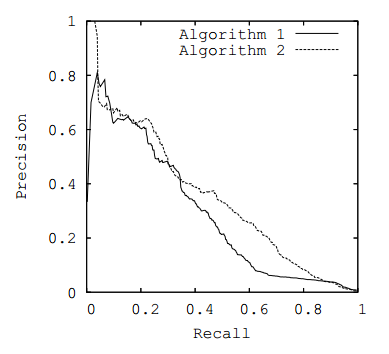
\includegraphics[scale=0.7]{./images/Prccurves.png}
\caption{\footnotesize{Due curve di due diversi algoritmi, generate dai diversi valori di Precision e Recall.}}
\label{prc_plot_ex}
\end{figure}

Per quanto riguarda le metriche centrate sui geni, si sono utilizzate la \emph{Fmax} (F-score gerarchica), massimizzata al variare di una soglia $t$ in $(0, 1)$. Tale misura si basa sulla Precisione e Recall centrate sui geni, che sono calcolate come:
\[
Precision(t) = \frac{1}{n}\sum_{j=1}^{n}\frac{TruePositive_{j}(t)}{TruePositive_{j}(t)+FalsePositive_j(t)}
\]
\[
Recall(t) = \frac{1}{n}\sum_{j=1}^{n} \frac{TruePositive_j(t)}{TruePositive_j(t)+FalseNegative_j(t)}
\]
dove $n$ è il numero di proteine/geni e $t$ è una soglia in $(0, 1)$. In sostanza sono delle Precision/Recall multi-etichetta mediate su tutti gli esempi. La Fmax viene poi calcolata come
\[
Fmax = \max_t\frac{2Precision(t)Recall(t)}{Precision(t)+Recall(t)}
\]
\section{Stime preliminari dei tempi di calcolo e delle performance}
Al fine di identificare delle configurazioni per gli esperimenti, capaci di terminare in tempi ragionevoli l'apprendimento e la valutazione delle performance, si sono eseguite delle stime preliminari sulla complessità temporale empirica dei modelli stessi.
\newline
\newline
La stima è stata effettuata su di un campione casuale di 10 classi (mostrate nella tabella \ref{selclss}) su ciascuno dei tre domini della Gene Ontology\footnote{\footnotesize{Biological Process, Molecular Function and Cellular Component.}}, eseguendo una \emph{cross-validation}\cite{niccross} a 10 fold.
\newline
\begin{table}[h]
\begin{tabular}{|l|l|l|l|l|l|}%
\hline
	\multicolumn{2}{|l|}{\textbf{Biological Process}}&\multicolumn{2}{|l|}{\textbf{Molecular Function}}&\multicolumn{2}{|l|}{\textbf{Cellular Component}}\\
	\hline
    \bfseries \small{Classe} & \bfseries \small{annotazioni} & \bfseries \small{Classe} & \bfseries \small{annotazioni} & \bfseries \small{Classe} & \bfseries \small{annotazioni}% specify table head
    \csvreader[head to column names]{csv_results/all_classes.csv}{}% use head of csv as column names
    {\\\hline \csvcoli&\csvcolii&\csvcoliii&\csvcoliv&\csvcolv&\csvcolvi}% specify your coloumns here
    \\\hline
    \end{tabular}
\caption{\footnotesize{Le classi selezionate nella fase preliminare, per ontologia}}
\label{selclss}
\end{table}


Per evitare di generare fold privi di esempi positivi, questi sono stati generati in maniera stratificata.\footnote{\footnotesize{Per generare i fold in maniera stratificata, si è sfruttata la funzione di R, \emph{do.stratified.cv.data.single.class\cite{stratified}}, presente nella libreria HEMDAG.}}.
\newline
\newline

\subsection{Risultati delle stime iniziali}
Le stime iniziali per l'intero processo di valutazione del learning, hanno evidenziato tempi di calcolo molto lunghi, nonostante sia stato escluso il tuning dei parametri di ogni algoritmo.
\newline
\newline
Come mostrato nelle tabelle \ref{BPtimes_p}, \ref{MFtimes_p} e \ref{CCtimes_p}, i tempi, che riguardano l'intero processo di cross-validation per alcuni algoritmi, sono sull'ordine delle ore per classe. Mantenendo questo set-up, prendendo ad esempio in considerazione solo le classi della BP ontology con almeno 10 annotazioni (1335), utilizzando l'algoritmo K-NN, servirebbero tra i 16 e i 17 mesi di computazione con i sistemi di calcolo disponibili per questo esperimento\footnote{\footnotesize{$9.16 h \times 1335 = 1228.9 h =~ 510 gg =~ 17months  $}}.
\newline
\newline
Dati i tempi molto lunghi riscontrati per i primi 6 algoritmi utilizzati\footnote{\footnotesize{C5.0, glmnet, knn, mlp, svmLinear, xgbLinear}}, si è preferito non proseguire ulteriormente con questa configurazione per le stime dei tempi di calcolo dei metodi rimanenti.
\newpage
\begin{table}[h]
\center
\begin{tabular}{|l|l|l|l|l|}%
\hline
    \bfseries Algo & \bfseries TempoMassimo & \bfseries TempoMinimo & \bfseries TempoMedio & \bfseries DevSt.Tempo % specify table head
    \csvreader[head to column names]{csv_results/BPtimes_.csv}{}% use head of csv as column names
    {\\\hline \csvcoli&\csvcolii&\csvcoliii&\csvcoliv&\csvcolv}\\\hline% specify your coloumns here
    \end{tabular}
\caption{\footnotesize{Alcune statistiche dei vari algoritmi per l'ontologia BP. I tempi sono da intendersi in ore e per classe, per un campione di 10 classi.}}
\label{BPtimes_p}
\end{table}

\begin{table}[h]
\center
\begin{tabular}{|l|l|l|l|l|}%
\hline
    \bfseries Algo & \bfseries TempoMassimo & \bfseries TempoMinimo & \bfseries TempoMedio & \bfseries DevSt.Tempo % specify table head
    \csvreader[head to column names]{csv_results/MFtimes_.csv}{}% use head of csv as column names
    {\\\hline \csvcoli&\csvcolii&\csvcoliii&\csvcoliv&\csvcolv}\\\hline% specify your coloumns here
    \end{tabular}
\caption{\footnotesize{Alcune statistiche dei vari algoritmi per l'ontologia MF. I tempi sono da intendersi in ore e per classe, per un campione di 10 classi.}}
\label{MFtimes_p}
\end{table}

\begin{table}[hp!]
\center
\begin{tabular}{|l|l|l|l|l|}%
\hline
    \bfseries Algo & \bfseries TempoMassimo & \bfseries TempoMinimo & \bfseries TempoMedio & \bfseries DevSt.Tempo % specify table head
    \csvreader[head to column names]{csv_results/BPtimes_.csv}{}% use head of csv as column names
    {\\\hline \csvcoli&\csvcolii&\csvcoliii&\csvcoliv&\csvcolv}\\\hline% specify your coloumns here
    \end{tabular}
\caption{\footnotesize{Alcune statistiche dei vari algoritmi per l'ontologia CC. I tempi sono da intendersi in ore e per classe, per un campione di 10 classi.}}
\label{CCtimes_p}
\end{table}
\newpage
Nei boxplot nella figura \ref{boxplot_p}, è possibile vedere come i tempi di calcolo varino (anche di molto) in base all'algoritmo utilizzato.

\begin{figure}[hp!]
\center
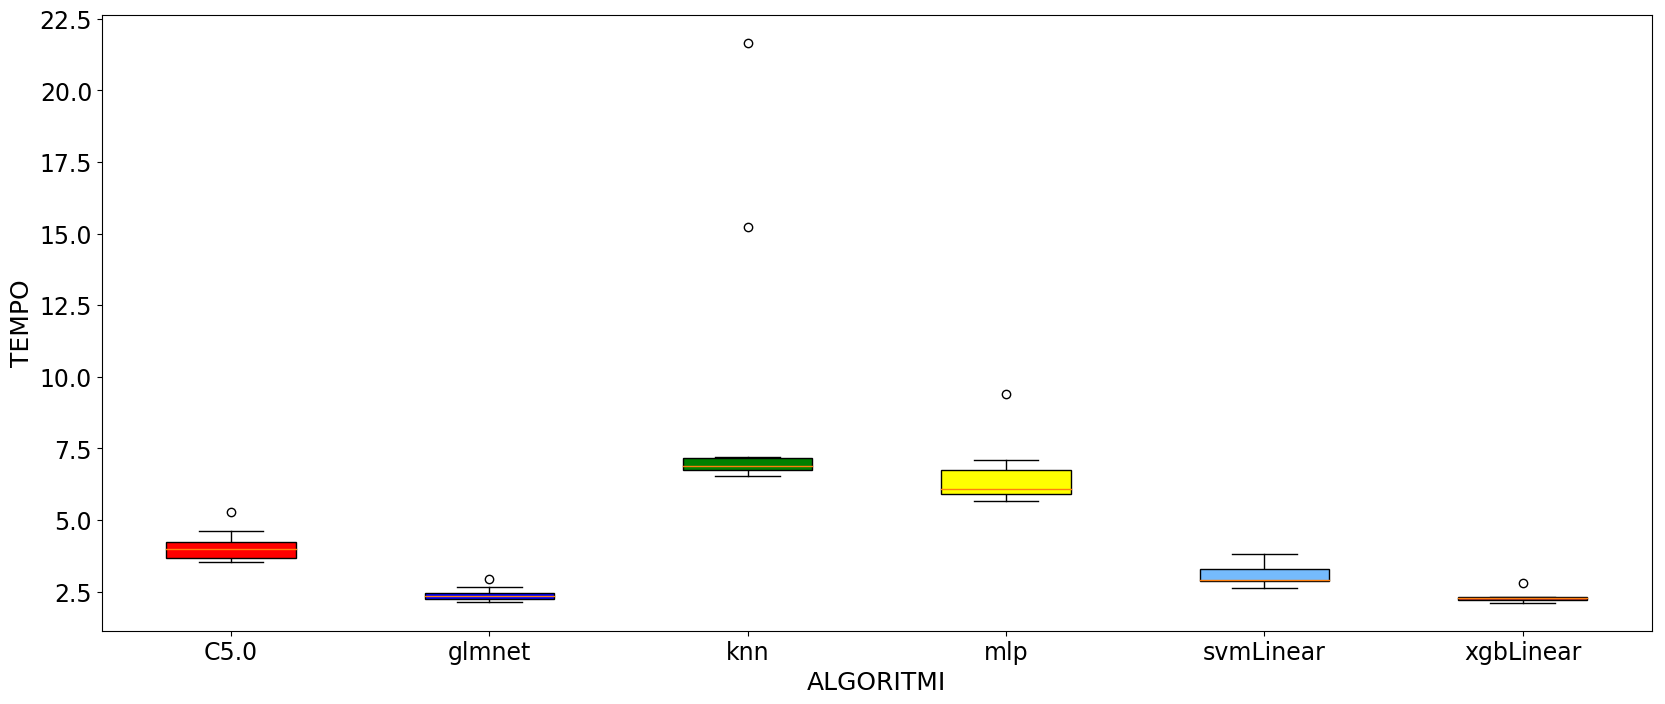
\includegraphics[scale=0.23]{images/BP_box_plot_times.png}
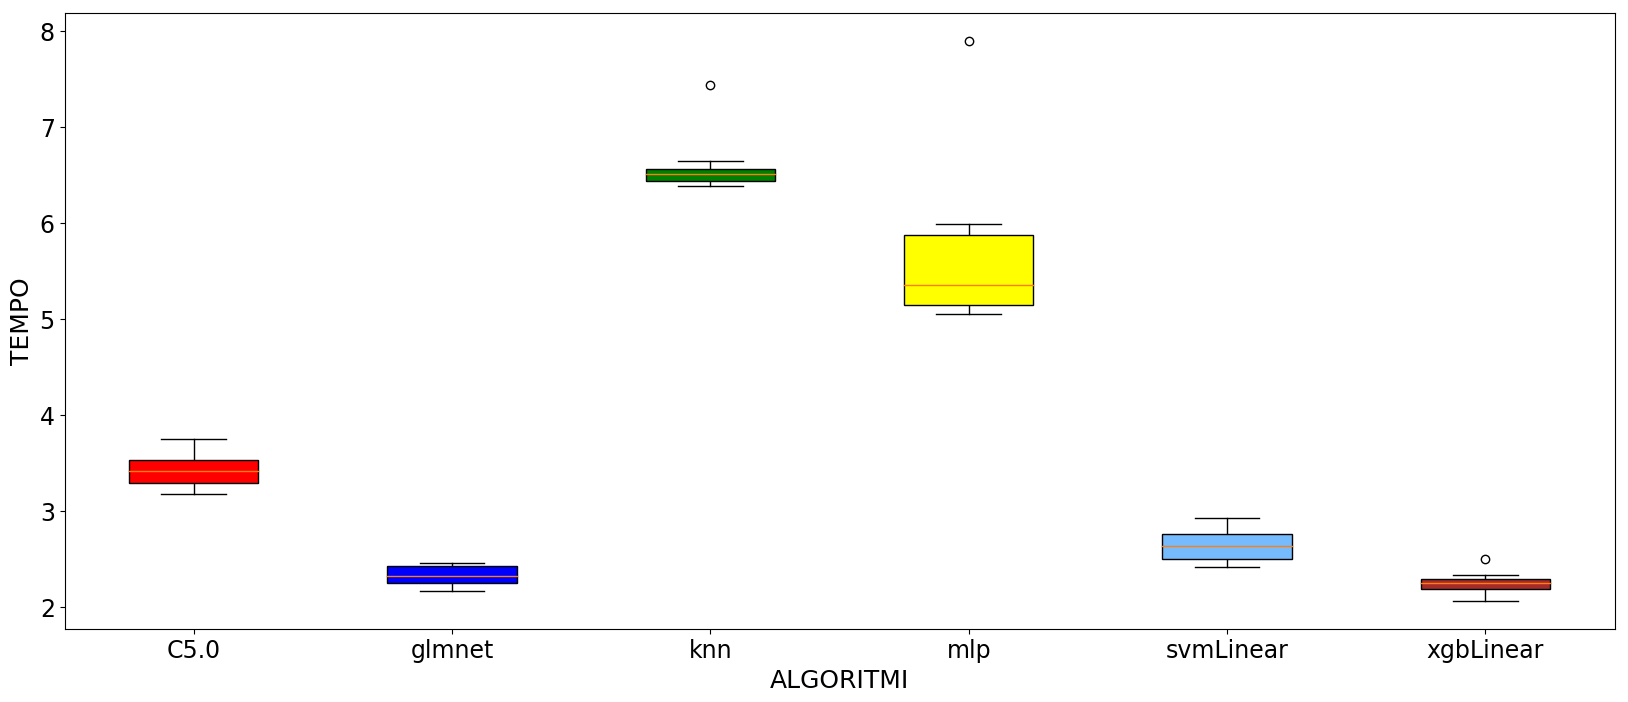
\includegraphics[scale=0.23]{images/MF_box_plot_times.png}
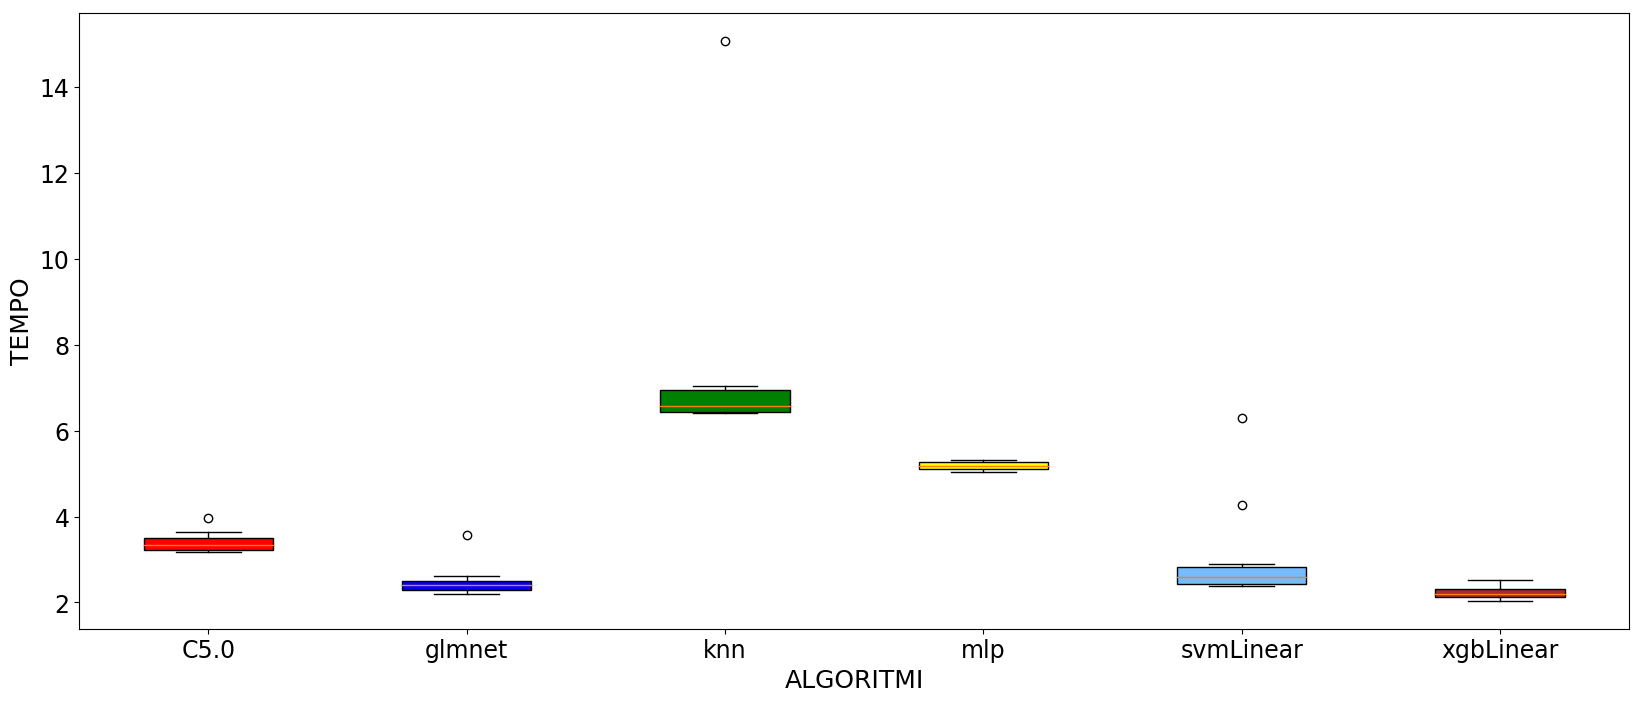
\includegraphics[scale=0.23]{images/CC_box_plot_times.png}
\caption{\footnotesize{I box plot dei tempi di esecuzione, con cross-validation a 10 fold per le ontologie BP, MF e CC. I tempi sono da intendersi in ore e per classe, per un campione di 10 classi.}}
\label{boxplot_p}
\end{figure}
Considerato quindi l'elevato numero di classi per ontologia, si è deciso di effettuare diverse operazioni volte a ridurre la complessità del problema, come la riduzione del numero di fold nella cross-validaton e delle feature da utilizzare nel processo di learning. 

\section{Riduzione della complessità del problema}
Verificati i tempi proibitivi nella fase iniziale esplorativa, si è deciso di effettuare due principali operazioni per ridurre la complessità dell'esperimento, e cioè:

\begin{itemize}
\item Introdurre la \emph{cross-validation a 5 fold} anziché a 10 fold per la stima delle performance.
\item Ridurre la complessità del learning con due metodi alternativi: \emph{Selezione delle feature} e \emph{PCA}.
\end{itemize} 

La riduzione della complessità non solo è utile a ridurre i tempi di calcolo dell'intero esperimento, ma ha lo scopo inoltre di ridurre il rischio di \emph{overfitting} dei modelli. Nel nostro caso specifico infatti, il numero di istanze del dataset risulta essere limitato in relazione al numero di feature (15752 istanze x 15752 feature) e parametri dei diversi modelli\cite{cesarid}.

\subsection{Selezione delle Feature}
Per la selezione delle feature si è deciso di utilizzare una selezione basata sulla \emph{Correlazione di Pearson}\cite{ROSS}, che ci permette di capire quanto una feature/caratteristica è \emph{correlata} con la classe di riferimento. 
\newline
\newline
Il calcolo della correlazione avviene tramite la seguente formula:
\[
corr_{X,Y} = \frac{COV(X,Y)}{\sigma_{X}\sigma_{Y}}
\]
Dove $X$ è ad esempio la variabile aleatoria che rappresenta l'annotazione delle istanze in relazione alla classe e $Y$ la variabile aleatoria che rappresenta il valore della feature (al variare delle istanze). $COV(X, Y)$ indica il valore di covarianza tra le variabili aleatorie e $\sigma$ la deviazione standard.
\newline
\newline
In questa maniera è possibile realizzare un \emph{ranking} (ordinamento) delle feature, in base al loro potenziale informativo. Un' alta correlazione, in valore assoluto, è infatti \emph{spesso}\footnote{\footnotesize{Non sempre un'alta correlazione implica una causalità, ma anzi può essere casuale.}} associata ad un grossa capacità predittiva della caratteristica.
\newline
\newline
Un altro motivo che ha portato all'utilizzo di questo tipo di selezione è la ridotta complessità temporale associata al calcolo della correlazione. Infatti, al fine di effettuare una selezione \emph{unbiased}\cite{unbiased}\footnote{\footnotesize{Effettuare una selezione delle feature a monte della cross-validation, porterebbe a dei problemi di \emph{data leakage}, in quanto si trasmetterebbe l'informazione presente nei test set dei diversi fold, nei training set, portando a delle stime delle performance con \emph{bias}.}}, tale selezione delle feature deve essere effettuata per ogni training set generato nella cross-validation. È chiaro quindi che se tale operazione diventa onerosa dal punto di vista computazionale\footnote{\footnotesize{TempoFeatureSelection $\times$ NumeroClassi $\times$ NumeroFoldCrossValidation}}, il vantaggio che ne deriva si riduce.

\subsection{Analisi delle componenti principali}
La \emph{PCA} è una tecnica che ci permette di individuare il sotto-spazio \emph{k-dimensionale} di $R^{d}$ \footnote{\footnotesize{Spazio di partenza in cui si trova il nostro dataset, con $d$ feature.}} in cui è massimizzata la varianza della componente principale\cite{cesarid}. Quindi fissato un $k$, il procedimento ci permette di estrarre le $k$ feature (in questo caso chiamate \emph{componenti}) del nuovo spazio. In questa maniera si può passare da uno spazio ad elevata dimensionalità ($d$ feature), ad uno con dimensionalità ridotta ($k$ componenti), con $k<<d$.
\newline
\newline
Concretamente il metodo genera le nuove $k$ componenti come combinazione lineare delle $d$ feature di partenza, in maniera tale da massimizzare la \emph{varianza spiegata}. Tutto ciò è reso possibile grazie ad un metodo di scomposizione matriciale, chiamato \emph{Singular Value Decomposition\cite{cesarid}}, che ci permette di individuare l'operatore lineare $P_k$, che risolve questo problema di minimo:
\[
min_{P_k\in P} ||X - P_{k}X||^{2}_F
\]
Dove $X$ è la matrice che rappresenta le nostre istanze, e l'operatore $|| . ||^{2}_F$ è la \emph{norma di Frobenius}, calcolata su di una matrice come:
\[
||X||^{2}_F = \sum_{i=1}^{m}\sum_{j=1}^{m} x_{ij}^2
\]

Un piccolo esempio di PCA lo possiamo vedere in figura \ref{pca_ex}\cite{pca_ref}.
\begin{figure}[hp!]
\center
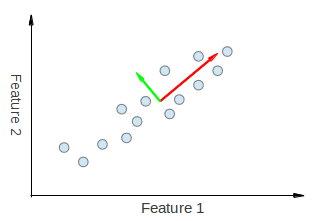
\includegraphics[scale=0.50]{./images/pca_eigen.png}
\caption{\footnotesize{Le feature iniziali sono la Feature 1 e la Feature 2. Le componenti ottenute dalla PCA sono il vettore in rosso e quello in verde. Se volessimo ridurre la dimensionalità di questo piccolo dataset, potremmo proiettare i punti sulla componente rossa (quella che massimizza la varianza) eliminando la componente verde.}}
\label{pca_ex}
\end{figure}
\newline
\newline
Le componenti risultate dall'analisi, si possono poi ordinare per varianza, la quale rappresenta il \emph{ranking} delle componenti del nuovo spazio vettoriale, e quindi il criterio di selezione per la riduzione della dimensionalità del problema.

\subsection{Stime dei tempi di calcolo e performance con selezione delle feature}
Per la selezione delle feature si è deciso di stimare i tempi di calcolo e le performance per 3 differenti livelli di selezione delle feature con cross-validation a 5 fold:
\begin{itemize}
\item Le prime 1000 feature nel ranking
\item Le prime 500 feature nel ranking
\item Le prime 100 feature nel ranking 
\end{itemize}

Come si può vedere dalla tabella \ref{featureSelection} in appendice, i tempi di calcolo ottenuti, sempre selezionando 10 classi per ognuna delle 3 ontologie (BP, MF, CC), per le selezioni delle feature a 1000 e 500 feature, risultano particolarmente alti, soprattutto per alcuni algoritmi (\emph{Adaboost, SvmLinear, LogitBoost e Treebag}).
\newline
\newline
Per questa motivazione si è deciso di optare per la selezione delle prime 100 feature nel ranking ottenuto dal calcolo della correlazione di Pearson. Nei boxplot in figura \ref{BPMFCCboxplotFStimes}, è possibile vedere come i tempi di calcolo si siano ridotti di molto a seguito della selezione delle prime 100 feature e con cross-validation a 5 fold. 
\begin{figure}[hp!]
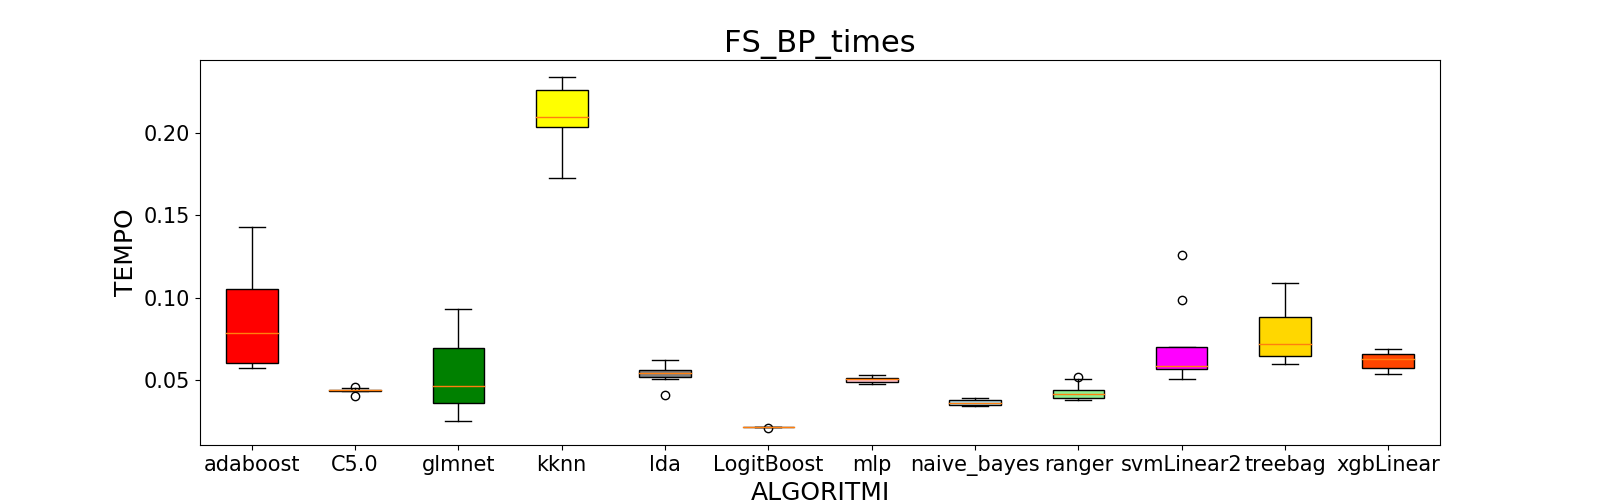
\includegraphics[scale=0.37]{./images/FS_BP_times.png}
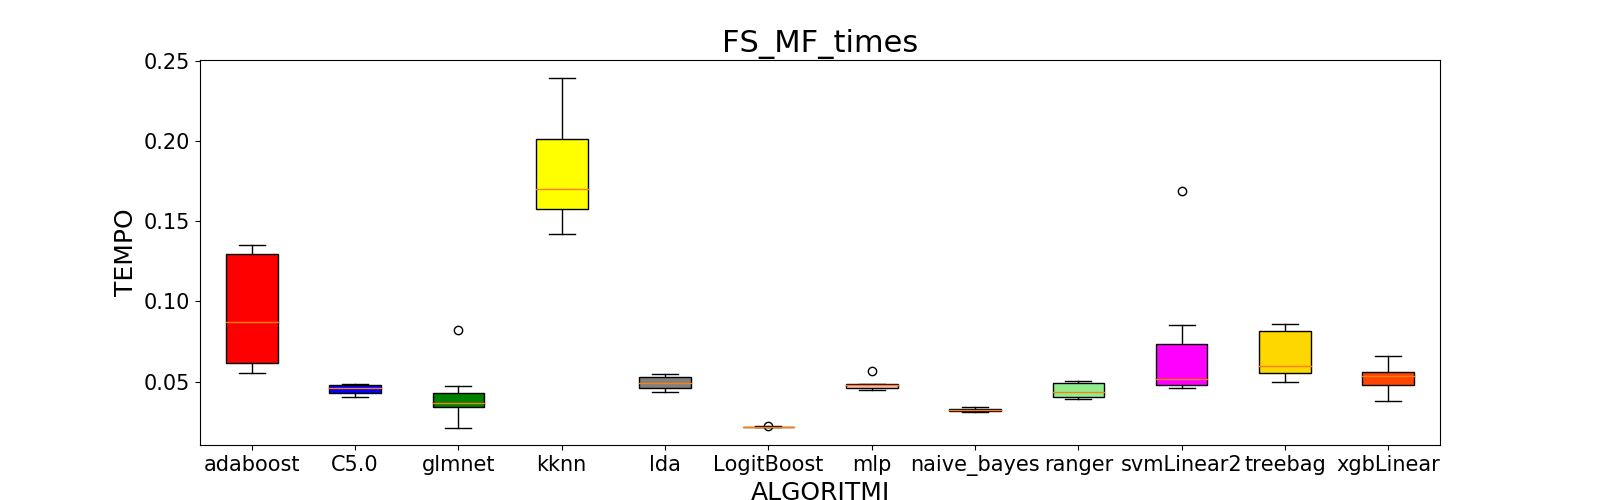
\includegraphics[scale=0.37]{./images/FS_MF_times.png}
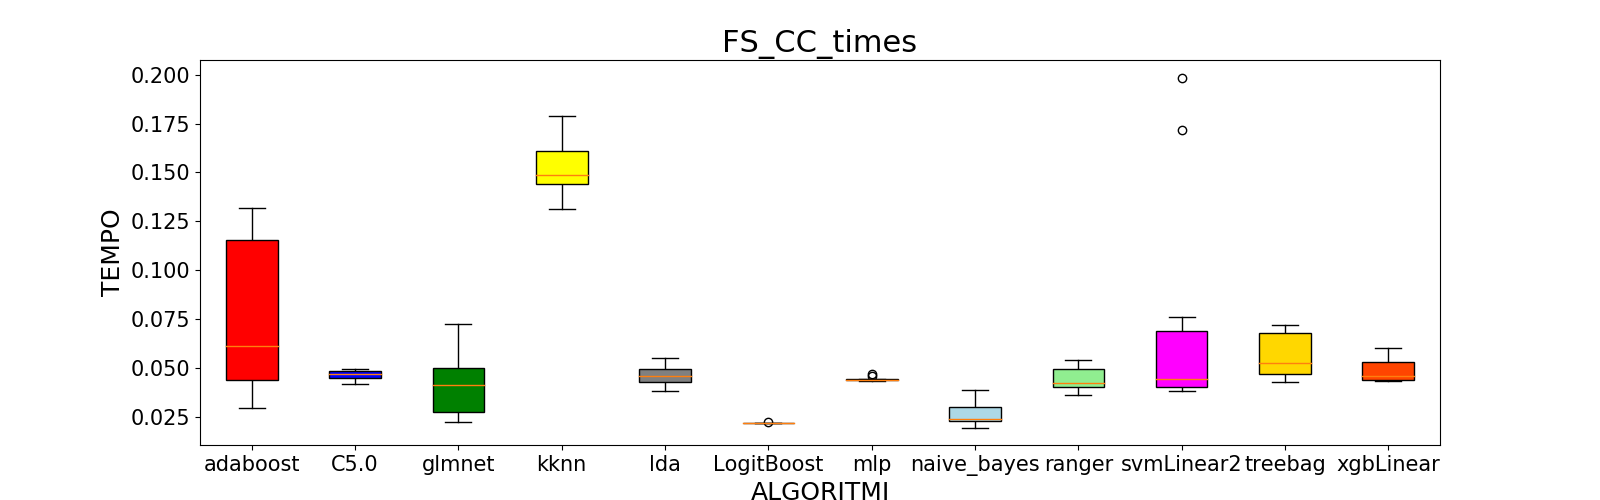
\includegraphics[scale=0.37]{./images/FS_CC_times.png}
\caption{\footnotesize{Boxplot dei tempi di calcolo dei diversi algoritmi per classe, su un campione di 10 classi, con selezione del prime 100 feature (correlazione di Pearson) e cross-validation a 5 fold, ontologie BP, MF e CC. I tempi sono da intendersi in ore.}}
\label{BPMFCCboxplotFStimes}
\end{figure}

Considerato il tempo medio per classe stimato e il numero totale delle classi, gli algoritmi più problematici a livello di tempo di calcolo risultano essere \emph{K-NN} (6 giorni di computazione),\emph{ Adaboost }(3 gg di computazione) e \emph{svmLinear} (meno di 3 giorni di computazione). Mentre a livello di performance non mostrano buoni risultati, vicino ad un predittore casuale, gli algoritmi \emph{glmnet}, \emph{C5.0}, \emph{K-NN}. Questo è probabilmente dovuto al fatto che si sono utilizzati i parametri di default delle librerie di caret senza effettuare una ricerca dei valori ottimali per lo specifico problema\footnote{\footnotesize{Lo scopo della tesi è di dimostrare empiricamente l'efficacia dei metodi ensemble a prescindere dei risultati flat.}}. \emph{Naive Bayes} mostra risultati scadenti per la metrica AUPRC, ma non per la AUROC, dove anzi ha risultati molto buoni. Nella figura \ref{BPMFCCboxplotfs5f} sono messe a confronto le performance stimate degli algoritmi, relative alla metrica AUROC, tramite boxplot, per le ontologie BP, MF e CC. Nella figura \ref{BPMFCCboxplotfs5fauprc} troviamo invece i boxplot per le stime della AUPRC.
\begin{figure}[hp!]
\centering
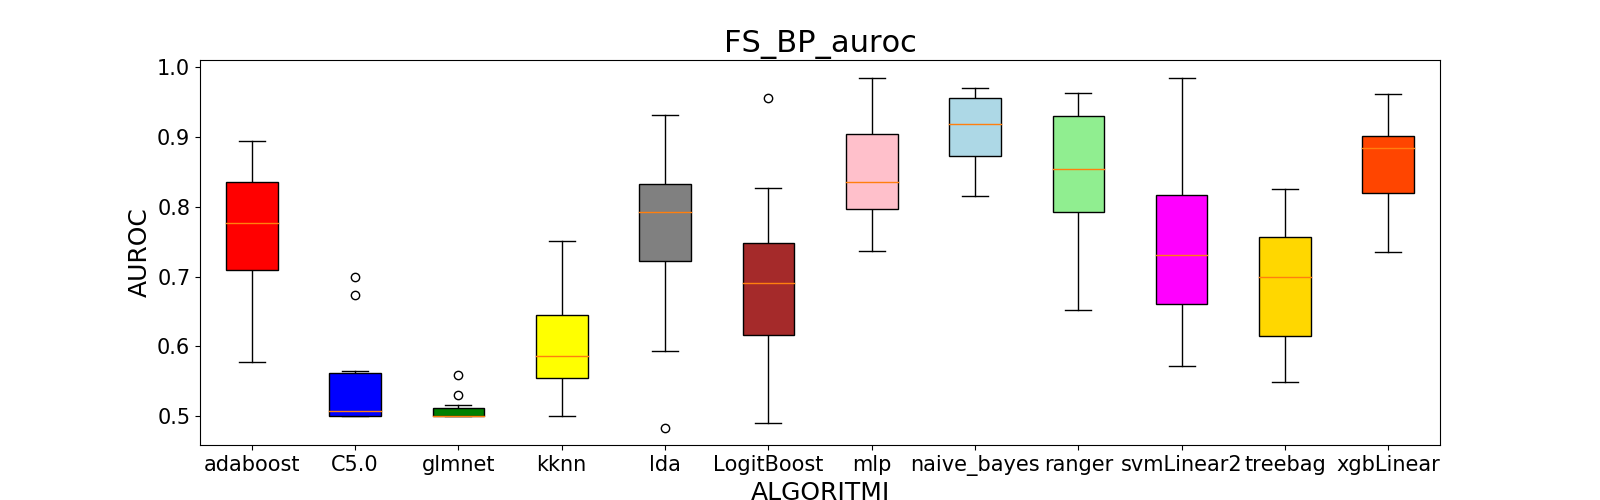
\includegraphics[scale=0.37]{./images/FS_BP_auroc.png}
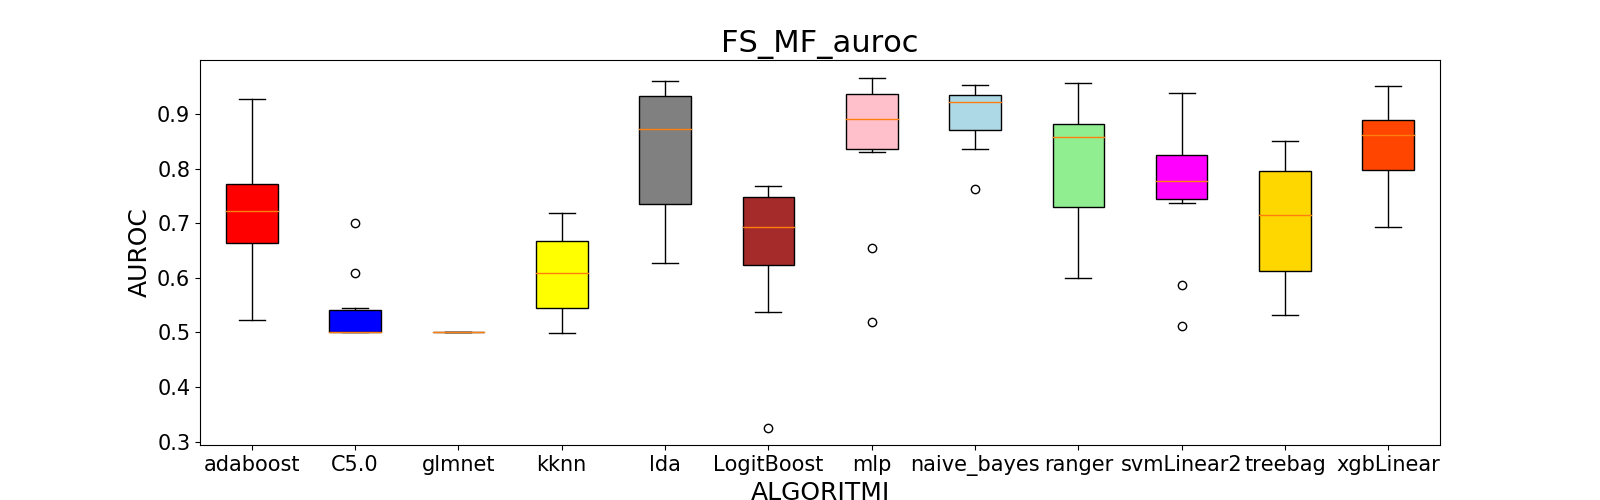
\includegraphics[scale=0.37]{./images/FS_MF_auroc.png}
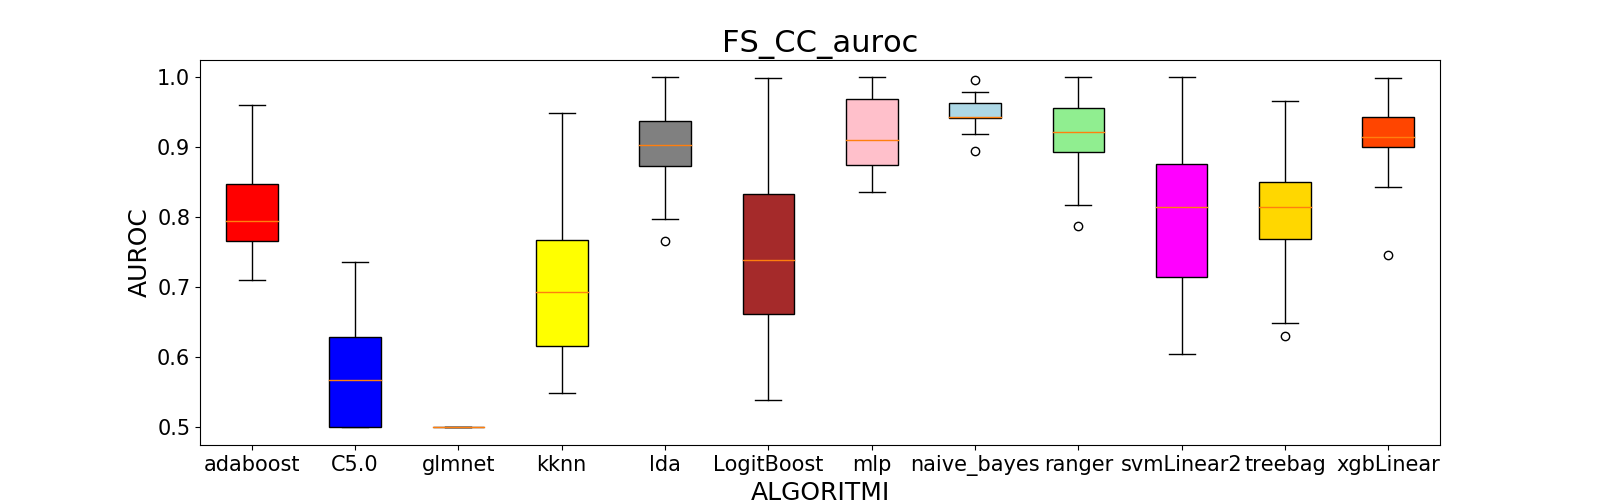
\includegraphics[scale=0.37]{./images/FS_CC_auroc.png}
\caption{\footnotesize{Boxplot delle performance di AUROC per classe dei diversi algoritmi, su un campione di 10 classi, con selezione del prime 100 feature (correlazione di Pearson) e cross-validation a 5 fold, per le ontologie BP, MF, CC. Sono evidenti le performance scadenti di \emph{C5.0}, \emph{glmnet} e \emph{K-NN}.}}
\label{BPMFCCboxplotfs5f}
\end{figure}

\begin{figure}[hp!]
\centering
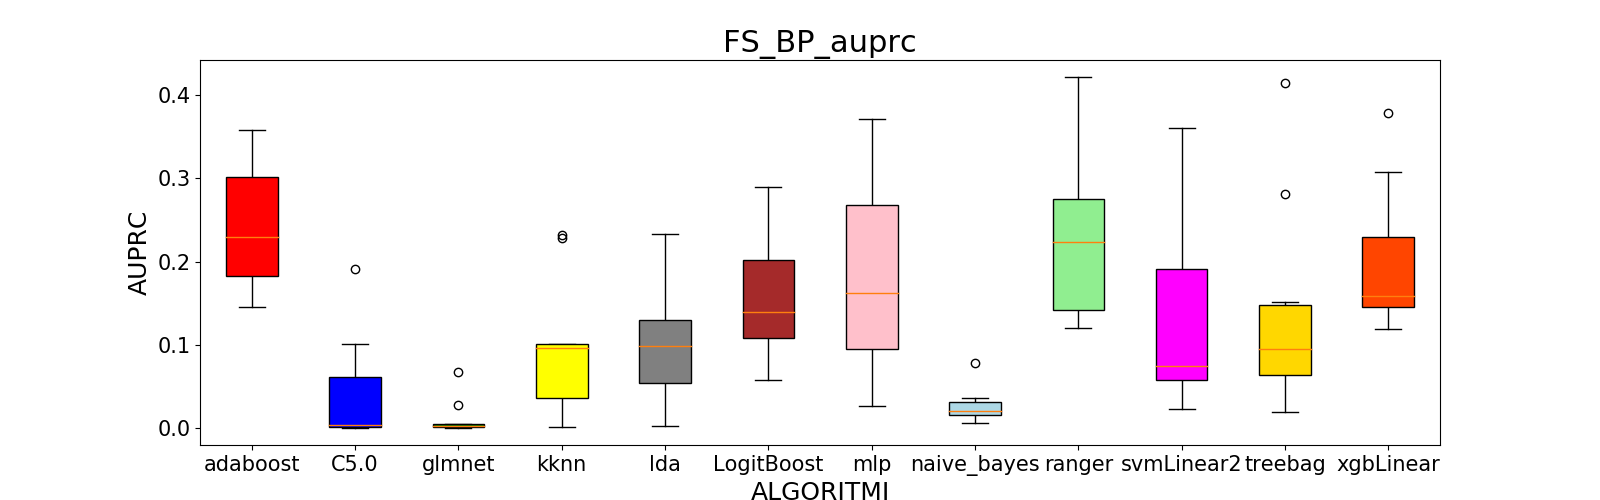
\includegraphics[scale=0.37]{./images/FS_BP_auprc.png}
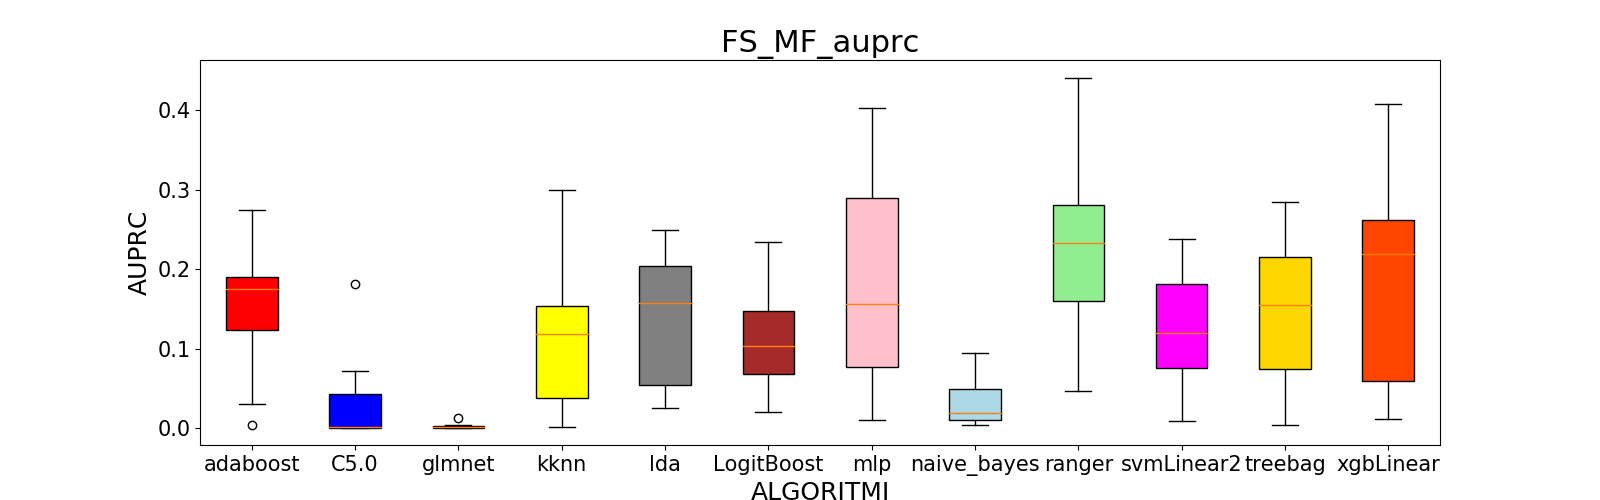
\includegraphics[scale=0.37]{./images/FS_MF_auprc.png}
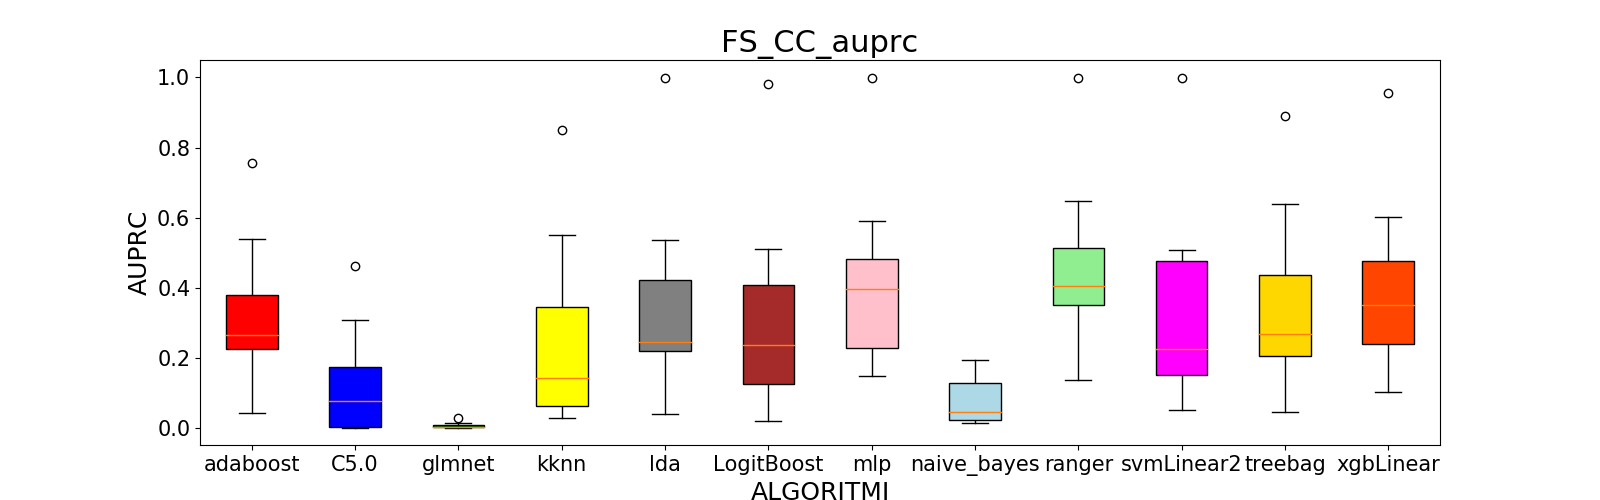
\includegraphics[scale=0.37]{./images/FS_CC_auprc.png}
\caption{\footnotesize{Boxplot delle performance di AUPRC per classe dei diversi algoritmi, su un campione di 10 classi, con selezione del prime 100 feature (correlazione di Pearson) e cross-validation a 5 fold, per le ontologie BP, MF, CC. Sono evidenti le performance scadenti di \emph{C5.0}, \emph{glmnet} e \emph{K-NN}, ma anche per l'algoritmo \emph{Naive Bayes}.}}
\label{BPMFCCboxplotfs5fauprc}
\end{figure}
\newpage
\subsection{Stime dei tempi di calcolo e performance con PCA}
L'operazione di generazione delle nuove componenti tramite PCA è stata effettuata per comodità sull'intera matrice delle istanze e non in maniera \emph{unbiased} come per la selezione delle feature, in quanto il \emph{data leakage} può essere trascurato, con una certa approssimazione, essendo l'analisi non supervisionata\footnote{Le classi sono escluse dall'analisi delle componenti.}. Dall'analisi dei risultati della PCA, mostrata nella figura \ref{varianceexplained}, emerge che gran parte della varianza può essere spiegata dalle prime componenti ottenute, le quali racchiudono gran parte dell'informazione.

\begin{figure}[hp!]
\centering
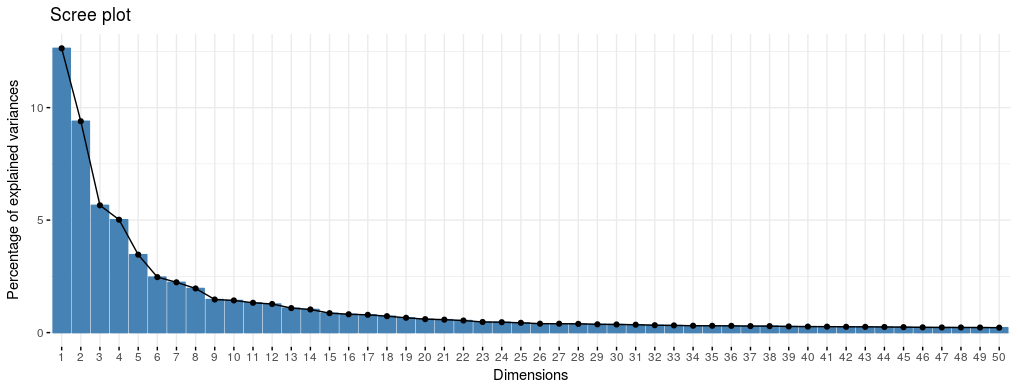
\includegraphics[scale=0.5]{./images/explained_variance.png}
\caption{\footnotesize{La varianza spiegata delle prime componenti. Come si può vedere dal grafico, l'informazione/varianza decresce piuttosto rapidamente.}}
\label{varianceexplained}
\end{figure} 

Per completezza si sono provati a stimare i tempi di calcolo e le performance di alcuni algoritmi, con 3 diversi livelli di varianza spiegata (con cross-validation a 10 fold), e cioè:
\begin{itemize}
\item 90\% di varianza spiegata: 1000 componenti
\item 70\% di varianza spiegata: 100 componenti
\item 50\% di varianza spiegata: 15 componenti
\end{itemize}
Come si può vedere dalla tabella \ref{diffvariance} in appendice , nella quale sono mostrate le stime, basate sempre sulla selezione di 10 classi per ontologia, le tempistiche diventano particolarmente lunghe sia per quanto riguarda la selezione con 1000 componenti, che con quella a 100 componenti.
\newline
\newline
Per questo motivo, si è deciso di selezionare le prime 15 componenti, che racchiudono circa il 50\% della varianza spiegata.
\newline
\newline
Effettuando le stime con questo tipo di selezione, introducendo inoltre una cross-validation a 5 fold, selezionando 10 classi randomicamente, i tempi si abbassano drasticamente, anche rispetto alla selezione di 100 feature con Pearson, come si può vedere dai box plot in figura \ref{timespcafs5}. Le performance non sono invece altrettanto positive, e anzi mostrano un netto calo generale, sia a livello di AUROC che AUPRC. Le stime sono mostrate nella tabella \ref{PCA5fold}.
\begin{figure}[hp!]
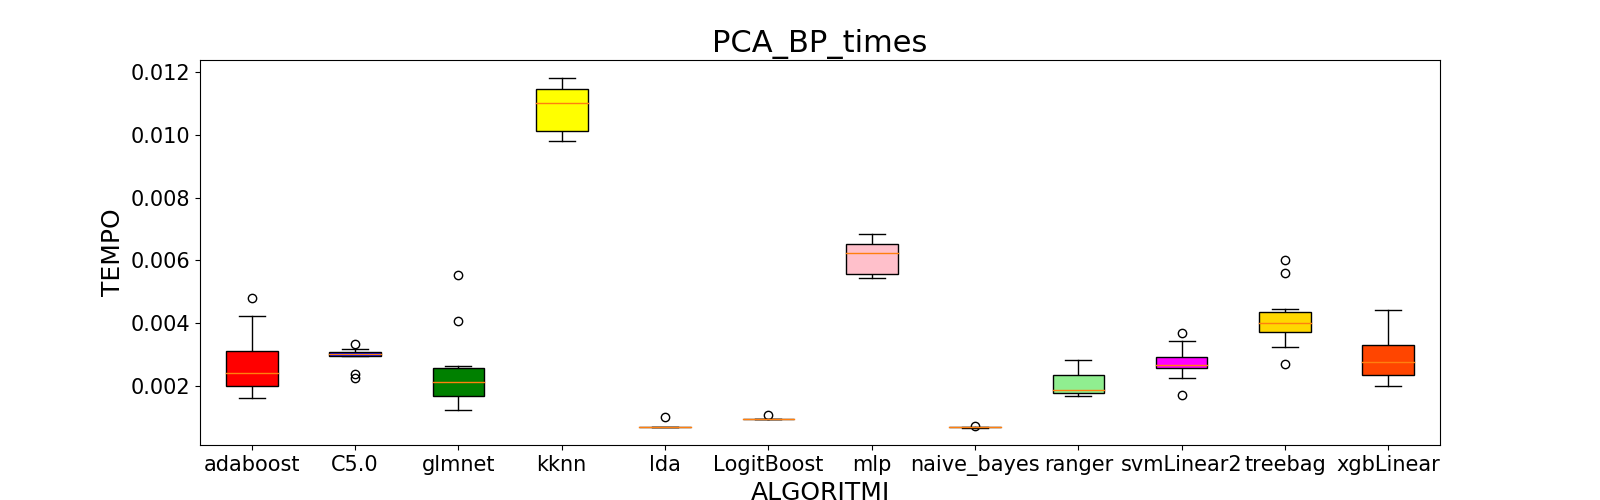
\includegraphics[scale=0.37]{./images/PCA_BP_times.png}
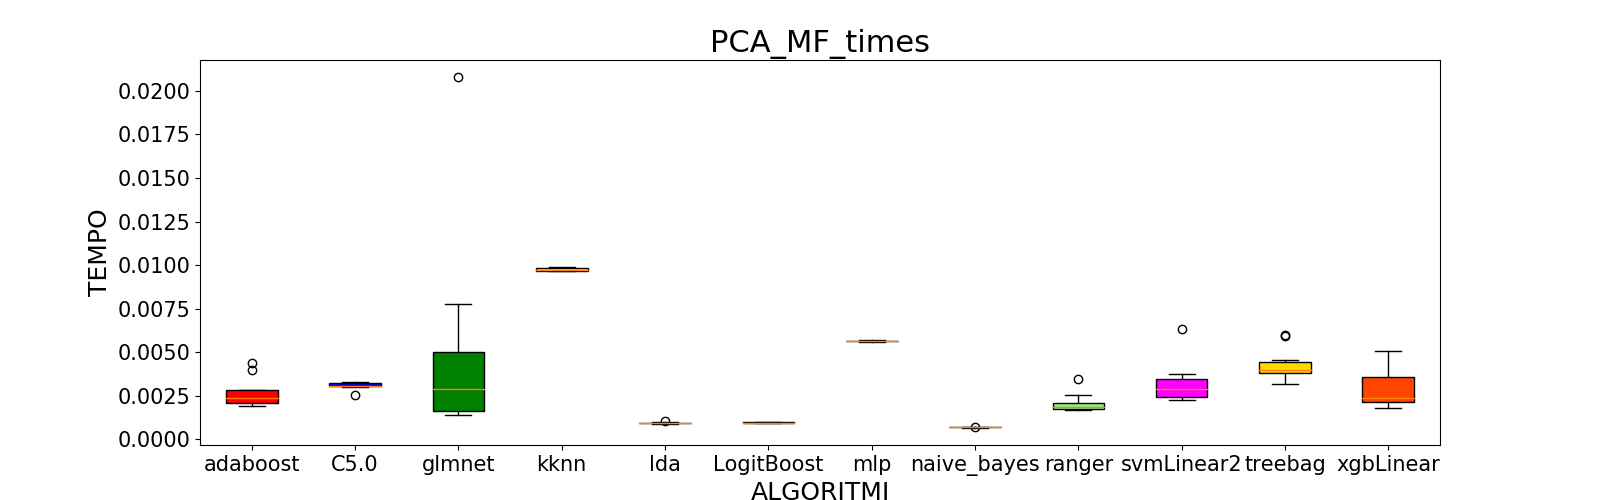
\includegraphics[scale=0.37]{./images/PCA_MF_times.png}
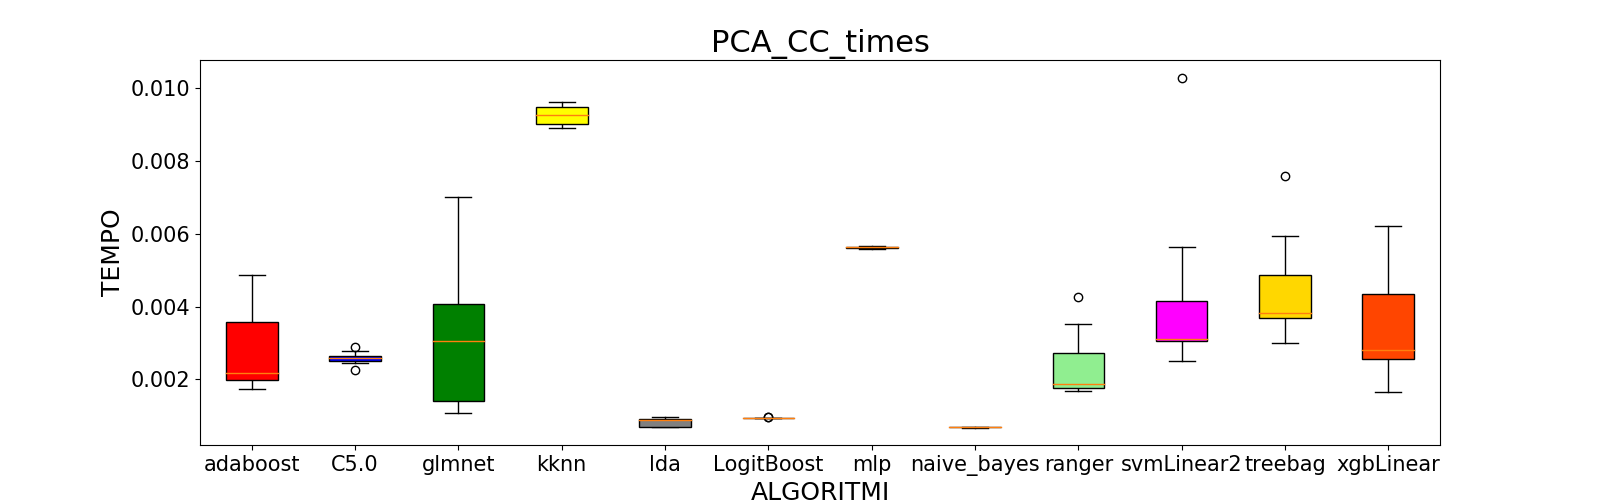
\includegraphics[scale=0.37]{./images/PCA_CC_times.png}
\caption{\footnotesize{Boxplot dei tempi di calcolo dei diversi algoritmi per classe, su un campione di 10 classi, con selezione delle prime 15 componenti della PCA e cross-validation a 5 fold, ontologie BP, MF e CC. I tempi sono da intendersi in ore.}}
\label{timespcafs5}
\end{figure}
\newline
\newline
Nelle figure \ref{BPboxplotpca5f} e \ref{BPboxplotpca5fauprc} sono mostrati i boxplot relativi alle performance di AUROC e AUPRC per gli algoritmi dell'esperimento. 
\begin{figure}[hp!]
\centering
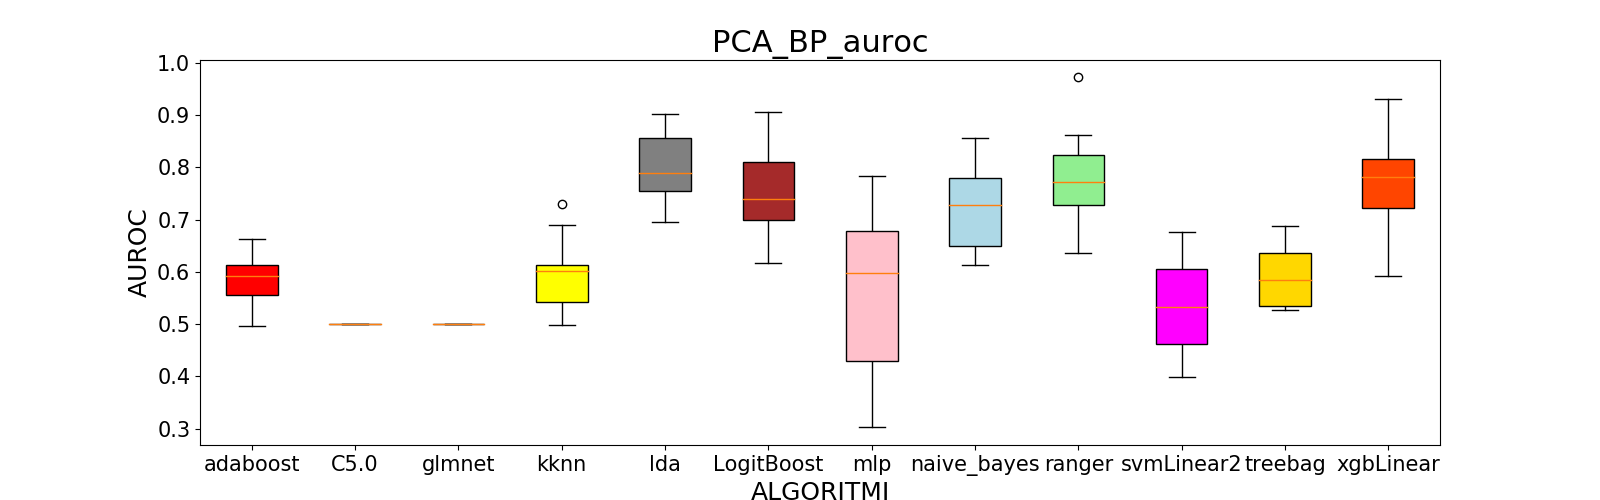
\includegraphics[scale=0.37]{./images/PCA_BP_auroc.png}
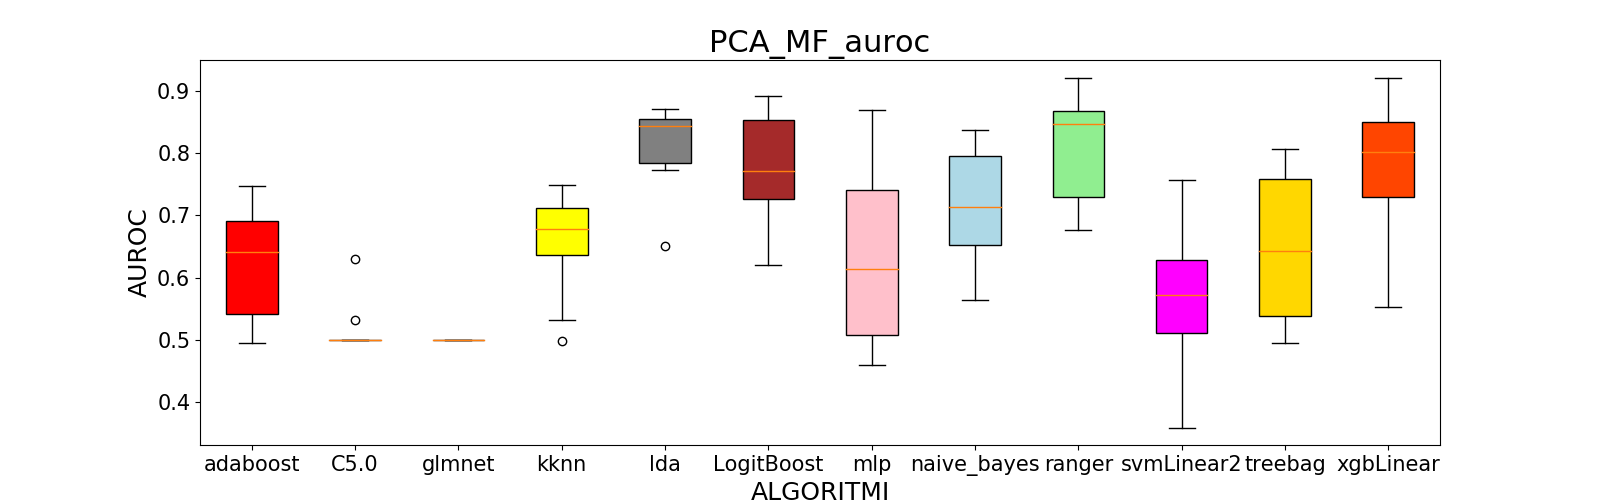
\includegraphics[scale=0.37]{./images/PCA_MF_auroc.png}
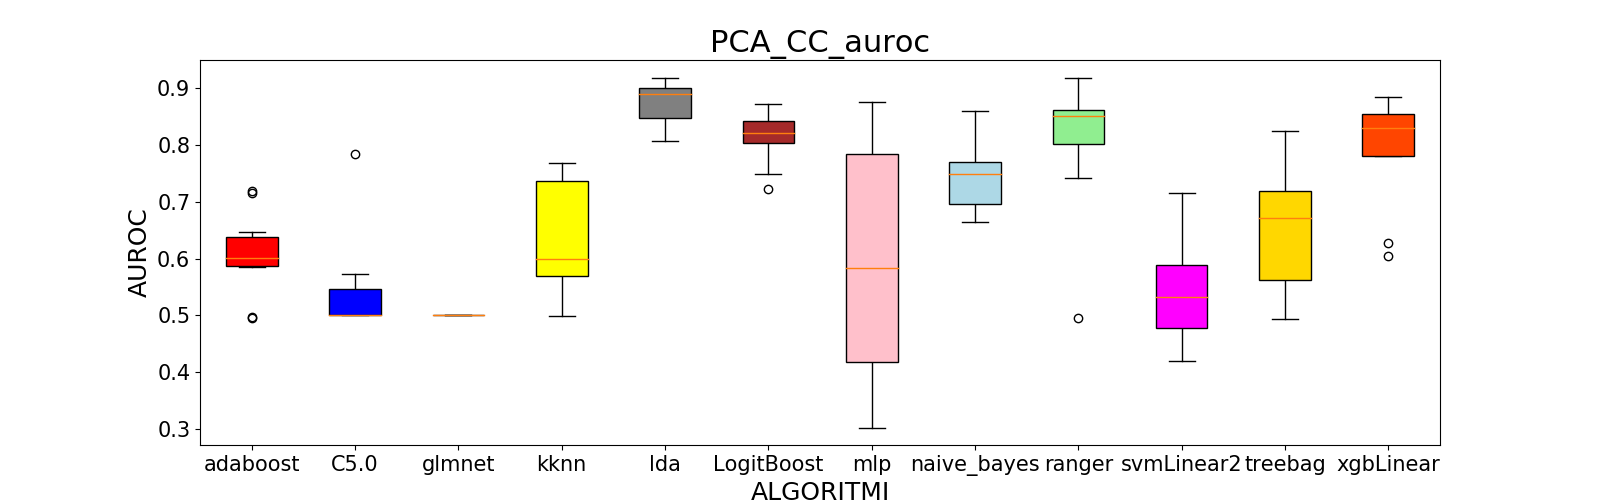
\includegraphics[scale=0.37]{./images/PCA_CC_auroc.png}
\caption{\footnotesize{Boxplot delle performance di AUROC per classe dei diversi algoritmi, su un campione di 10 classi, con selezione delle prime 15 componenti e cross-validation a 5 fold, per le ontologie BP, MF, CC.}}
\label{BPboxplotpca5f}
\end{figure}

\begin{figure}[hp!]
\centering
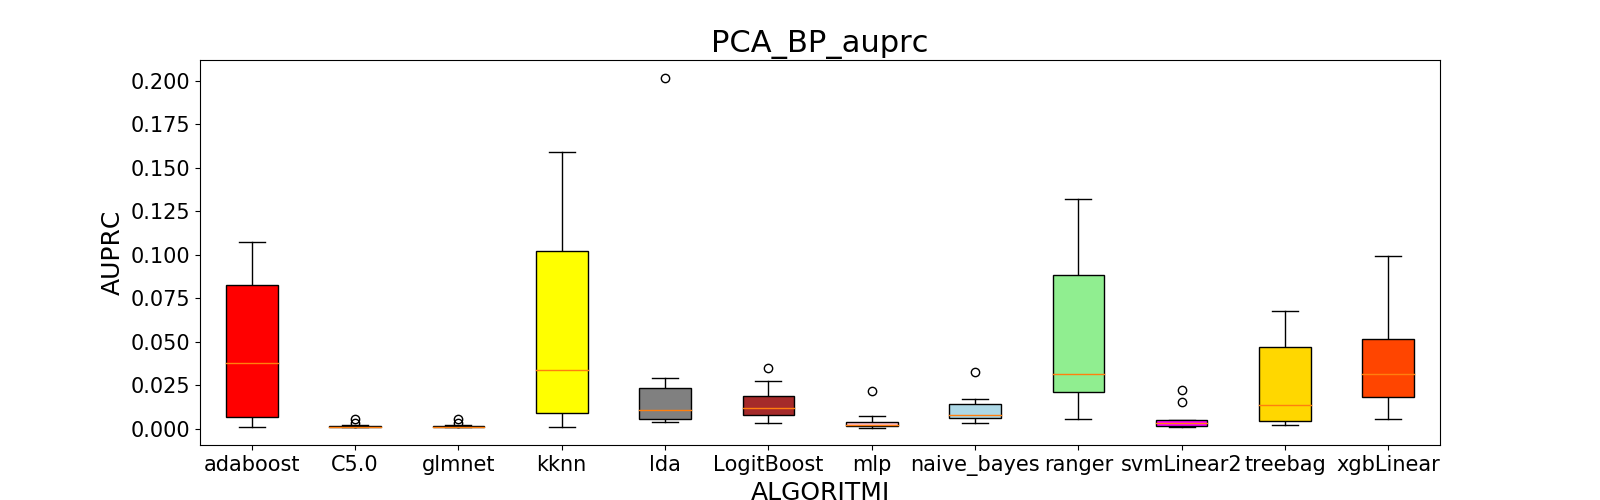
\includegraphics[scale=0.37]{./images/PCA_BP_auprc.png}
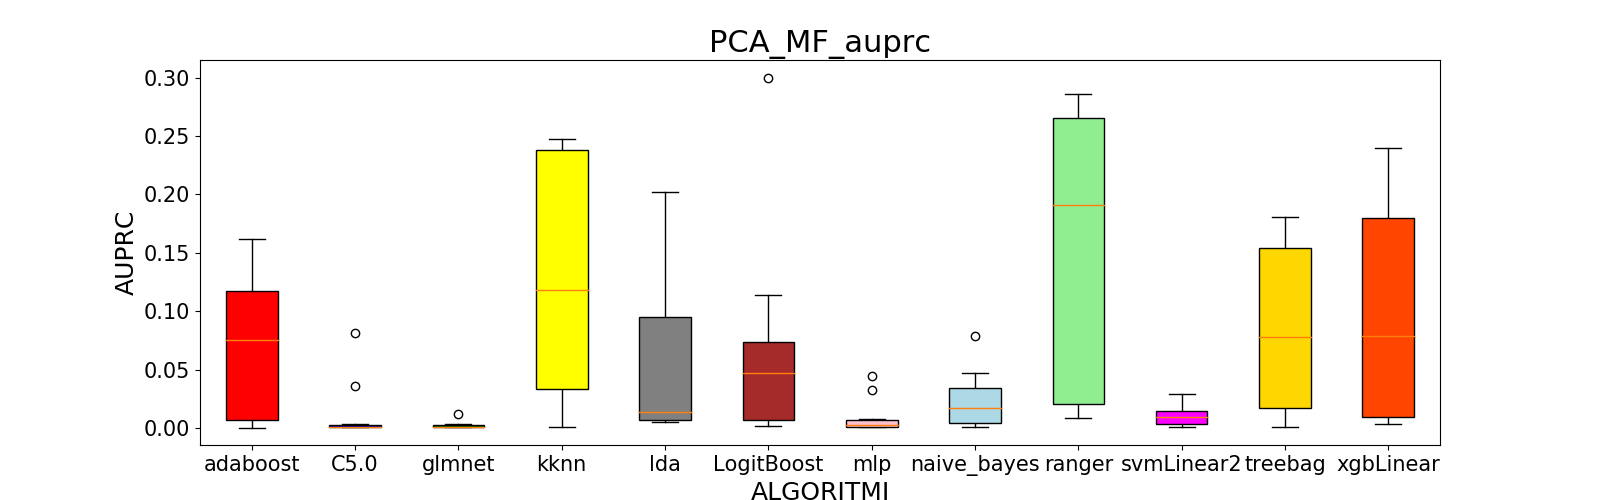
\includegraphics[scale=0.37]{./images/PCA_MF_auprc.png}
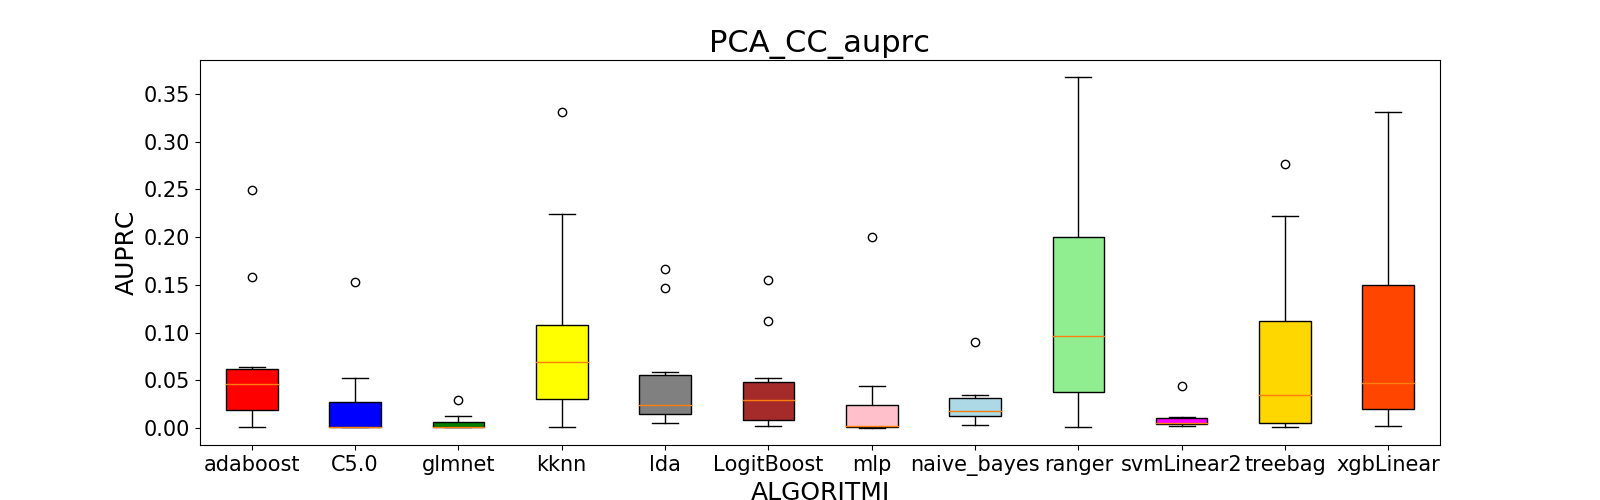
\includegraphics[scale=0.37]{./images/PCA_CC_auprc.png}
\caption{\footnotesize{Boxplot delle performance di AUPRC per classe dei diversi algoritmi, su un campione di 10 classi, con selezione delle prime 15 componenti e cross-validation a 5 fold, per le ontologie BP, MF, CC.}}
\label{BPboxplotpca5fauprc}
\end{figure}
\newpage
\section{Organizzazione degli esperimenti}
Si sono divisi gli esperimenti in due blocchi principali:
\begin{enumerate}
\item Predizioni flat con i 12 diversi algoritmi di apprendimento specificati in partenza. 
\item Applicazione di diversi metodi di correzione gerarchica.
\end{enumerate}

Data l'analisi precedente effettuata sugli algoritmi di apprendimento flat, che ha evidenziato, tramite delle stime, tempi di calcolo troppo elevati, si è deciso di generare le predizioni flat di tutte le classi delle tre ontologie\footnote{\footnotesize{Come si è specificato in preccedenza, si sono escluse dal grafo delle ontologie quelle classi che hanno meno di 10 annotazioni.}}, con due configurazioni principali:

\begin{itemize}
\item cross-validation 5 fold + Selezione delle prime 100 feature con Correlazione di Pearson.
\item cross-validation 5 fold + Selezione delle prime 15 componenti della PCA.
\end{itemize} 
Si è deciso per queste selezioni in quanto le stime iniziali hanno evidenziato un buon compromesso tra tempi di esecuzione e performance.  
\newline
\newline
A seguito della generazione dei risultati flat, si è effettuata poi la correzione gerarchica tramite i seguenti metodi di ensemble gerarchico:

\begin{enumerate}
\item HTD-DAG (top-down)
\item GPAV (top-down)
\item TPR-DAG (bottom-up + top-down)
\item ISO-TPR (bottom-up + top-down)
\end{enumerate}

Per gli ultimi due metodi (TPR-DAG, ISO-TPR), si sono considerate le seguenti varianti di selezioni dei figli e aggiornamento delle predizioni:
\begin{itemize}
\item Senza soglia (\emph{Threshold Free} - TF)
\item Con soglia variabile (\emph{Adaptive Threshold} - AT)
\item Con pesi (\emph{Weighted} - W)
\end{itemize}

La selezione senza soglia genera l'insieme dei figli $\phi$ di un nodo $i$ tale che
\[
\phi_i = \{j \in child(i) | \bar{y}_j > \hat{y}_i \}
\]
e cioè comprende tutti quei figli che hanno un valore per la predizione superiore a quella del genitore.
\newline
\newline
La selezione dei figli con soglia variabile  si ottiene cercando di massimizzare una metrica $M$, che valuta le performance del metodo gerarchico, al variare di una soglia $t$ in $(0,1)$, come 
\[
\phi_i = \{j \in child(i) | \bar{y}_j \geq t_j^{*}, t_j^{*} = arg\;\max_{t} M(j, t)   \}
\]
. Nel nostro caso come metrica $M$ è stata utilizzata la \emph{Fmax}, i cui valori ottimali $t^{*}$  si sono ottenuti tramite cross-validazione (con 5 fold) sul training set.
\newline
\newline
Infine, l'aggiornamento pesato comporta l'introduzione di un peso $w$, che ci indica in che misura il genitore e i figli contribuiscono alla correzione $\bar{y}_i$ della predizione $\hat{y}_i$, che viene calcolata come
\[
\bar{y}_i = w \hat{y}_i + \frac{(1-w)}{|\phi_i|}\sum_{j \in \phi_i}\bar{y}_j
\]
Così come per la soglia $t$ per la metrica $M$ nella soglia adattiva, anche per il peso $w$ è stata eseguita una cross-validazione a 5 fold per l'individuazione dei suoi valori ottimali. Per mantenere bassa la complessità del problema, l'insieme dei figli $\phi_i$ nel metodo pesato è ottenuto con il metodo di selezione senza soglia (TF). Per diminuire il carico computazionale, l'aggiornamento con peso è stato applicato al solo metodo gerarchico TPR-DAG.

\section{Predizioni flat}
La generazione di tutti gli score flat, per entrambi i metodi di riduzione della complessità, ha evidenziato delle performance generalmente migliori per la selezione delle feature effettuta con la correlazione di Pearson. Le performance migliori sono probabilmente da ricondurre al fatto che il tipo di riduzione per la correlazione è \emph{supervisionato} a differenza della PCA.
\newline
\newline
Nella figura \ref{versusAUROC} sono messi a confronto i risultati degli algoritmi a coppie, con feature selection e con PCA, per la metrica AUROC, tramite dei boxplot. Nella figura \ref{versusAUPRC}troviamo invece i risultati per la AUPRC, sempre tramite boxplot.

\begin{figure}[h!]
\centering
\hspace*{-0.9in}
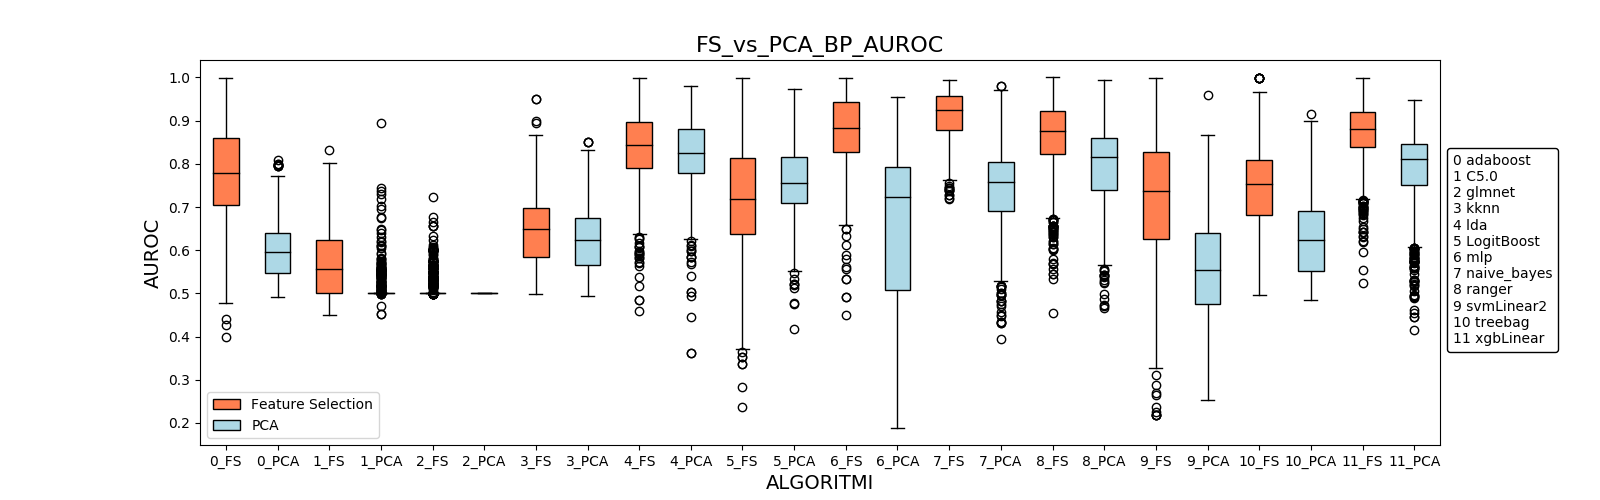
\includegraphics[scale=0.43]{./images/FS_vs_PCA_BP_AUROC.png}
\hspace*{-0.9in}
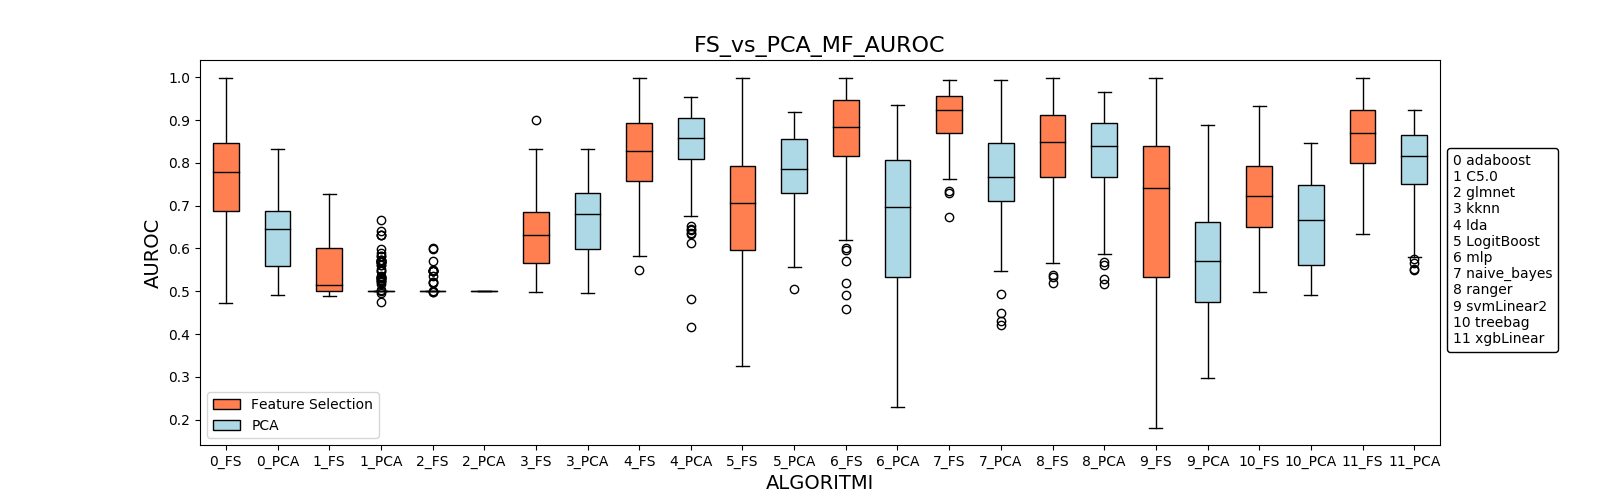
\includegraphics[scale=0.43]{./images/FS_vs_PCA_MF_AUROC.png}
\hspace*{-0.9in}
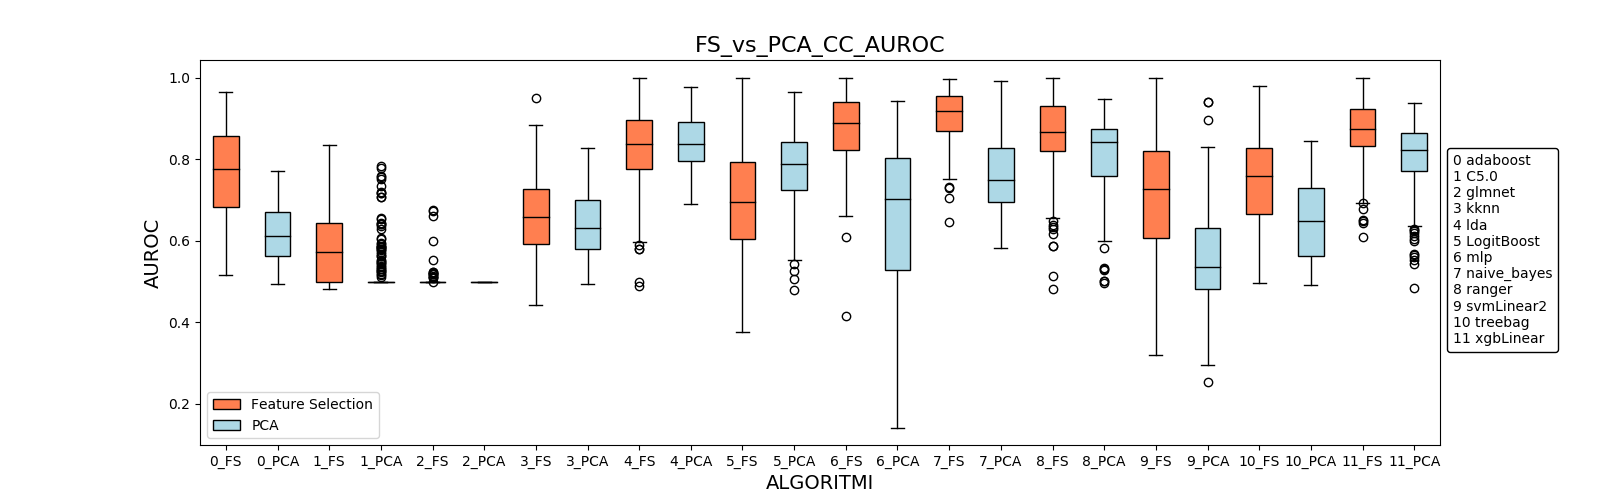
\includegraphics[scale=0.43]{./images/FS_vs_PCA_CC_AUROC.png}
\caption{\footnotesize{I risultati della AUROC per algoritmo, alternando selezione delle feature a PCA, per le tre ontologie in sequenza (BP, MF, CC). In ordine abbiamo: Adaboost, C5.0, glmnet, knn, lda, Logit Boost, mlp, naive bayes, Random Forest, Svm , tree bag, xgbLinear.}}
\label{versusAUROC}
\end{figure}

\begin{figure}[h!]
\centering
\hspace*{-0.9in}
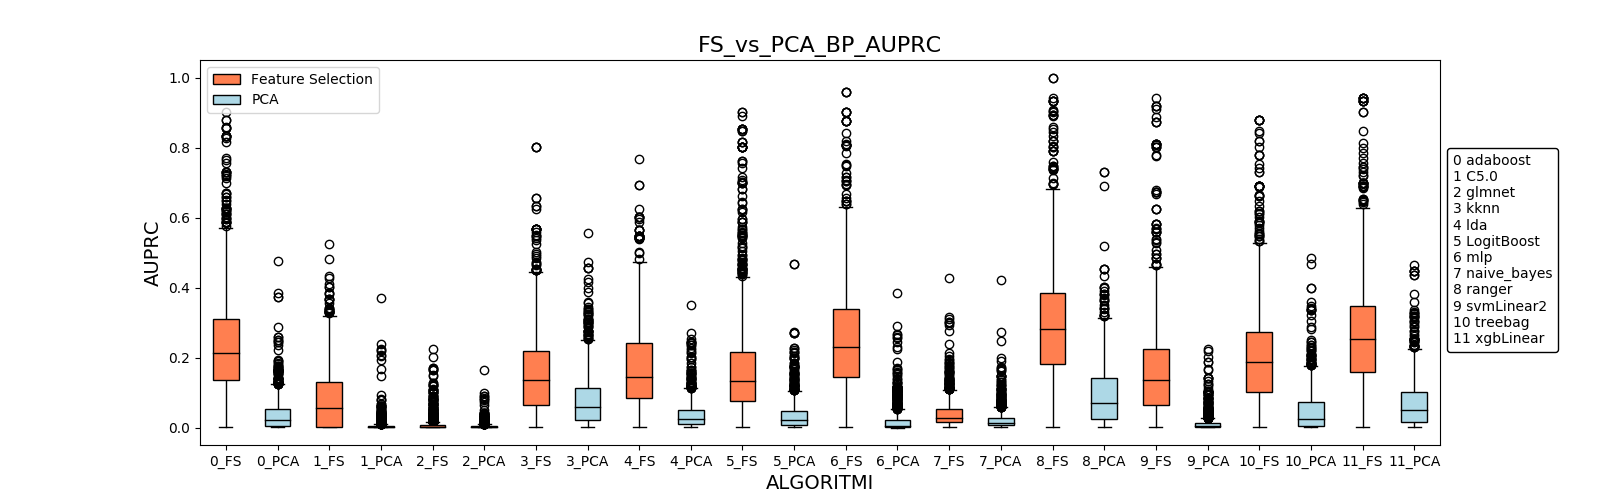
\includegraphics[scale=0.43]{./images/FS_vs_PCA_BP_AUPRC.png}
\hspace*{-0.9in}
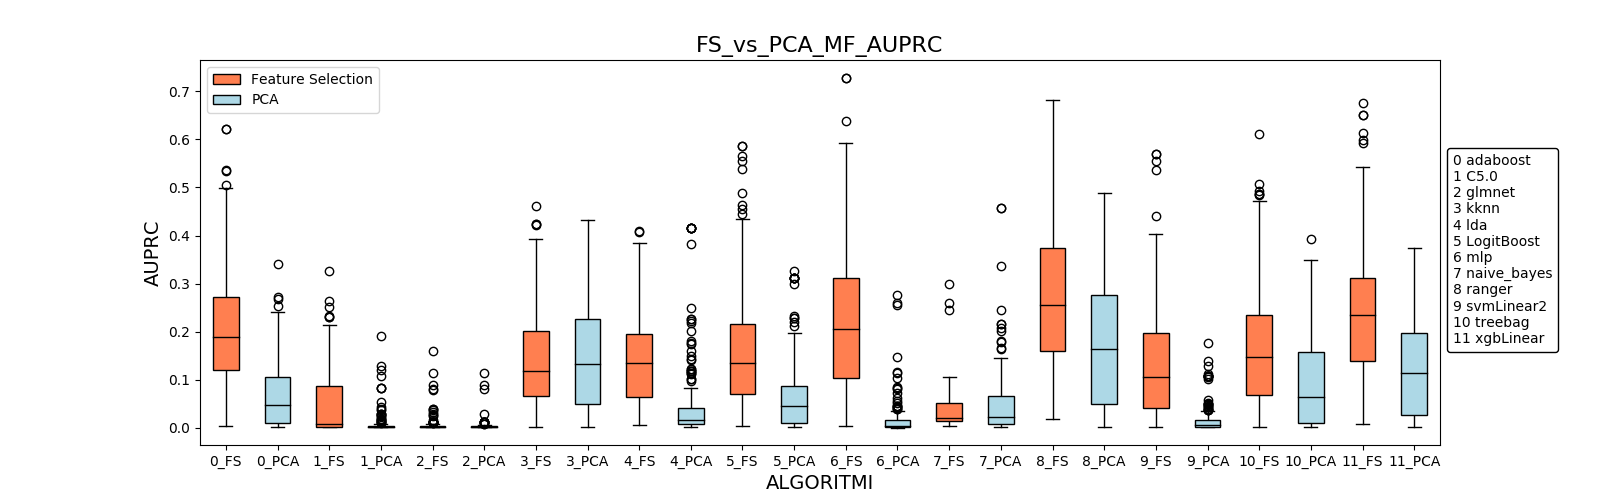
\includegraphics[scale=0.43]{./images/FS_vs_PCA_MF_AUPRC.png}
\hspace*{-0.9in}
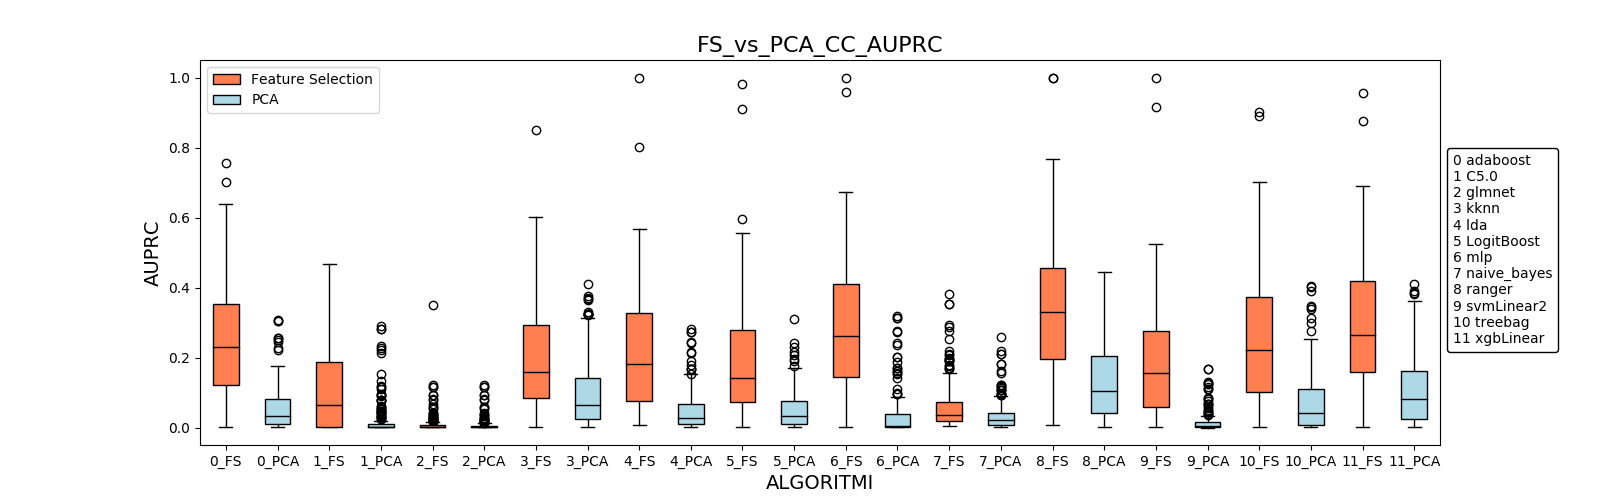
\includegraphics[scale=0.43]{./images/FS_vs_PCA_CC_AUPRC.png}
\caption{\footnotesize{I risultati della AUPRC per algoritmo, alternando selezione delle feature a PCA, per le tre ontologie in sequenza (BP, MF, CC). In ordine abbiamo: Adaboost, C5.0, glmnet, knn, lda, Logit Boost, mlp, naive bayes, Random Forest, Svm , tree bag, xgbLinear}}
\label{versusAUPRC}
\end{figure}

Le differenze maggiori sono evidenti soprattutto per la metrica AUPRC, dove difficilmente la PCA (con selezione della varianza al 50\%) riesce a essere competitiva. 
\newline
\newline
Per verificare inoltre se la differenza in performance tra selezione delle feature e PCA è statisticamente significativa, sono stati effettuati dei test di ipotesi sui campioni dei risultati ottenuti dai due metodi di riduzione della dimensionalità del problema.
\newline
\newline
Come test di ipotesi è stato utilizzato quello di Kolmogorov e Smirnov\cite{ROSS}, un test \emph{non parametrico} e a due code, che ci permette di verificare la probabilità che due campioni provengono dalla stessa popolazione senza fare assunzioni sul tipo di distribuzione.
\newline
\newline
Dato il livello di significatività del test $a=0.05$ e come ipotesi nulla $H_0$ l'appartenenza dei due campioni alla medesima popolazione, sono quindi stati effettuati dei test a due a due sui campioni ottenuti variando il metodo di riduzione della dimensionalità del problema, fissato un algoritmo. Come si può vedere dalle tabelle \ref{AUROC_FS_vs_PCA} e \ref{AUPRC_FS_vs_PCA}, che mostrano rispettivamente i p-value ottenuti per la metrica AUROC e per la metrica AUPRC, i casi in cui l'ipotesi nulla non viene scartata (p-value $>= a$), fanno riferimento prevalentemente all'algoritmo \emph{glmnet}. Questo è dovuto probabilmente ai risultati dell'algoritmo che, a causa del mancato tuning, porta a risultati vicini a quelli di un predittore casuale. Un altro algoritmo che genera risultati statisticamente indistinguibili al variare del metodo di riduzione della dimensionalità è \emph{K-NN}, per l'ontologia MF. In tutti gli altri casi si può dire, con una confidenza del 95\%, che gli algoritmi producono popolazioni (e quindi risultati) differenti. Consequenzialmente si può affermare che in generale il metodo di selezione delle feature genera performance migliori.
\begin{table}[h]
\centering
\hspace*{-0.3in}
\resizebox{.8\textwidth}{!}{
\begin{tabular}{|l|l|l|l|l|l|l|}
\hline
\textbf{Onto\textbackslash{}Algo} & \textbf{adaboost} & \textbf{C5.0}         & \textbf{glmnet} & \textbf{knn}       & \textbf{lda}     & \textbf{LogitBoost} \\ \hline
\textbf{BP}                       & 0                 & 0                     & 0               & 0                   & 0                & 0                   \\ \hline
\textbf{MF}                       & 0                 & 0                     & 0,65118         & 7E-05               & 0,00337          & 0                   \\ \hline
\textbf{CC}                       & 0                 & 0                     & 0,67381         & 0,02319             & 0,03078          & 0                   \\ \hline
\textbf{Onto\textbackslash{}Algo} & \textbf{mlp}      & \textbf{naiveBayes} & \textbf{ranger} & \textbf{svm} & \textbf{treebag} & \textbf{xgbLinear}  \\ \hline
\textbf{BP}                       & 0                 & 0                     & 0               & 0                   & 0                & 0                   \\ \hline
\textbf{MF}                       & 0                 & 0                     & 0,02632         & 0                   & 5E-05            & 0                   \\ \hline
\textbf{CC}                       & 0                 & 0                     & 0               & 0                   & 0                & 0                   \\ \hline
\end{tabular}}
\caption{\footnotesize{P-value ottenuti dal test di kolmogorov per la metrica AUROC. Fissato l'algoritmo (colonna) si può identificare il p-value relativo ad una specifica ontologia (riga). Il p-value fa riferimento ai due campioni delle performance (AUROC) ottenuti dallo stesso algoritmo, variando il tipo di riduzione della dimensionalità (Selezione delle feature e PCA).}}
\label{AUROC_FS_vs_PCA}
\end{table}


\begin{table}[h]
\centering
\hspace*{-0.3in}
\resizebox{.9\textwidth}{!}{
\begin{tabular}{|l|l|l|l|l|l|l|}
\hline
\textbf{Onto\textbackslash{}Algo} & \textbf{adaboost} & \textbf{C5.0}       & \textbf{glmnet} & \textbf{knn} & \textbf{lda}     & \textbf{LogitBoost} \\ \hline
\textbf{BP}                       & 0                 & 0                   & 0               & 0            & 0                & 0                   \\ \hline
\textbf{MF}                       & 0                 & 0                   & 0,73899         & 0,13797      & 0                & 0                   \\ \hline
\textbf{CC}                       & 0                 & 0                   & 0,94171         & 0            & 0                & 0                   \\ \hline
\textbf{Onto\textbackslash{}Algo} & \textbf{mlp}      & \textbf{naiveBayes} & \textbf{ranger} & \textbf{svm} & \textbf{treebag} & \textbf{xgbLinear}  \\ \hline
\textbf{BP}                       & 0                 & 0                   & 0               & 0            & 0                & 0                   \\ \hline
\textbf{MF}                       & 0                 & 0,0023              & 0               & 0            & 0                & 0                   \\ \hline
\textbf{CC}                       & 0                 & 0                   & 0               & 0            & 0                & 0                   \\ \hline
\end{tabular}}
\caption{\footnotesize{P-value ottenuti dal test di kolmogorov per la metrica AUPRC. Fissato l'algoritmo (colonna) si può identificare il p-value relativo ad una specifica ontologia (riga). Il p-value fa riferimento ai due campioni delle performance (AUPRC) ottenuti dallo stesso algoritmo, variando il tipo di riduzione della dimensionalità (Selezione delle feature e PCA).}}
\label{AUPRC_FS_vs_PCA}
\end{table}
\newpage
\section{Predizioni strutturate}
Nelle figure \ref{BP_AUC_1}, \ref{BP_AUC_2}, \ref{MF_AUC_1}, \ref{MF_AUC_2}, \ref{CC_AUC_1} e \ref{CC_AUC_2} in appendice, sono mostrati i boxplot delle performance dei diversi metodi, in relazione alla metrica AUROC, fissati gli algoritmi, al variare dell'ontologia e del metodo di riduzione della dimensionalità del problema. Visivamente è possibile intuire come i metodi ensemble tendano a migliorare i risultati flat, e ad essere più efficaci, quando è utilizzata la selezione delle feature come metodo di riduzione della dimensionalità. Questo è dovuto probabilmente al fatto che i risultati flat ottenuti con selezione delle feature siano migliori rispetto a quelli ottenuti con PCA, come si è verificato empiricamente nel capitolo precedente delle predizioni flat. Non è invece facile comprendere se esiste, in questo contesto, un metodo gerarchico generalmente superiore ad un altro. Sono evidenti invece le scarse performance del metodo HTD, che anzi, spesso risulta essere peggiorativo anche rispetto ai metodi flat.
\newline
\newline
La situazione è visivamente del tutto simile all'AUROC per la metrica AUPRC, come mostrato nei box plot \ref{BP_PRC_1}, \ref{BP_PRC_2}, \ref{MF_PRC_1}, \ref{MF_PRC_2}, \ref{CC_PRC_1} e \ref{CC_PRC_2} in appendice. Non vi è infatti un metodo ensemble dominante, e anzi dipende dal contesto (ontologia, algoritmo di ML e metodo di riduzione della dimensionalità). Anche qui HTD mostra risultati non del tutto positivi, e, come per l'AUROC, ci sono situazioni in cui la performance del metodo risulta peggiorativa in relazione agli score flat.  

\subsection{Metodi Flat vs Metodi Ensemble Gerarchici}
Per verificare se esistono differenze statisticamente significative tra le performance dei metodi gerarchici e quelle degli algoritmi flat, si è eseguito il test dei ranghi con segno di Wilcoxon\cite{wilcoxon}(\emph{Paired Wilcoxon signed-rank test}). Tale test è \emph{non parametrico}, in quanto non fa assunzioni sulla distribuzione delle differenze di performance tra i metodi, ma assume ci sia dipendenza tra le coppie estratte dalla popolazione\footnote{\footnotesize{Assume che ci sia ad esempio un dipendenza del tipo \emph{prima} - \emph{dopo}, che nel nostro caso si può tradurre come \emph{metodo flat}(prima) -  \emph{metodo gerarchico}(dopo).}}.
\newline
\newline
Si sono quindi raggruppati i risultati per ontologia e metodo di riduzione della dimensionalità, e si sono confrontate le performance dei metodi flat e dei diversi metodi di correzione gerarchica, assumendo come ipotesi nulla $H_0$ la condizione che i due campioni provengano dalla stessa popolazione.
\newline
\newline 
Dato il numero di test di ipotesi elevato da effettuare per gruppo (12 per algoritmo flat base), al fine di evitare di identificare dei falsi positivi,  si è applicata la correzione di Bonferroni\cite{bonferr} al p-value. Data quindi una significatività finale desiderata $\alpha=0.01$, ogni test $i$ è stato effettuato con un livello di significatività $\alpha_i$ pari a $\alpha/12$ \footnote{\footnotesize{Senza correzione di Bonferroni, la probabilità di identificare un falso positivo con una significatività $\alpha = 0.01$ e 12 test di ipotesi, è pari a $1-(0.99^{12}) = 0.11 > 0.01$.}}.
\newline
\newline
Effettuando i confronti per ontologia, metodo di riduzione della dimensionalità e metrica osservata, si sono generate quindi le tabelle \ref{test_ipotesi1}(AUROC) e \ref{test_ipotesi2}(AUPRC), nelle quali è mostrato il numero di volte in cui l'ipotesi nulla viene rifiutata (performance metodo flat $\neq$ performance metodo gerarchico) e il metodo gerarchico risulta essere superiore al metodo flat. Per stabilire se un metodo gerarchico è superiore ad un metodo flat a livello di performance si è confrontato il valore atteso stimato (media campionaria) delle due popolazioni per la metrica osservata. 
\newline
\newline
È interessante notare come i metodi gerarchici risultino più efficaci quando la riduzione della dimensionalità è avvenuta tramite l'utilizzo della correlazione di Pearson, per entrambe le metriche AUROC e AUPRC. Infatti, ad eccezione del metodo gerarchico HTD, i metodi gerarchici risultano essere molto spesso\footnote{\footnotesize{In un range che va tra le 10, 11, 12 volte su 12}} migliorativi rispetto agli algoritmi flat base, quando la selezione è avvenuta tramite la correlazione di Pearson. Guardando invece al solo algoritmo TPR-AT (TPR-DAG con soglia adattiva), questo sembra essere più efficace quando si osserva la metrica AUPRC, ma risulta non sempre migliorativo quando si guarda alla AUROC.

\begin{table}[h!]
\hspace*{0.6in}
\caption*{\textbf{Confronto fra metodi gerarchici e metodi flat (AUROC).}}
\hspace*{0.6in}
                    \resizebox{.3\textwidth}{!}{
                    \begin{subtable}[t]{0.4\textwidth}
                    \centering\footnotesize
\caption{ \textbf{[AUROC] [BP] [FS]}}
\begin{tabular}{|l|l|}
\hline
 \textbf{WIN / LOSE} & \textbf{flat} \\ \hline
 \textbf{GPAV} & 12/12 \\ \hline
 \textbf{HTD} & 1/12 \\ \hline
 \textbf{TPR-TF} & 11/12 \\ \hline
 \textbf{ISO-TPR-TF} & 12/12 \\ \hline
 \textbf{TPR-AT} & 5/12 \\ \hline
 \textbf{ISO-TPR-AT} & 11/12 \\ \hline
 \textbf{TPR-W} & 11/12 \\ \hline
\end{tabular}

                    \label{table1}
                    \end{subtable}}
\hspace*{0.6in}
                    \resizebox{.3\textwidth}{!}{
                    \begin{subtable}[t]{0.4\textwidth}
                    \centering\footnotesize
\caption{ \textbf{[AUROC] [BP] [PCA]}}
\begin{tabular}{|l|l|}
\hline
 \textbf{WIN / LOSE} & \textbf{flat} \\ \hline
 \textbf{GPAV} & 8/12 \\ \hline
 \textbf{HTD} & 7/12 \\ \hline
 \textbf{TPR-TF} & 9/12 \\ \hline
 \textbf{ISO-TPR-TF} & 6/12 \\ \hline
 \textbf{TPR-AT} & 7/12 \\ \hline
 \textbf{ISO-TPR-AT} & 6/12 \\ \hline
 \textbf{TPR-W} & 10/12 \\ \hline
\end{tabular}

                    \label{table1}
                    \end{subtable}}\par\bigskip

\hspace*{0.6in}
                    \resizebox{.3\textwidth}{!}{
                    \begin{subtable}[t]{0.4\textwidth}
                    \centering\footnotesize
\caption{ \textbf{[AUROC] [MF] [FS]}}
\begin{tabular}{|l|l|}
\hline
 \textbf{WIN / LOSE} & \textbf{flat} \\ \hline
 \textbf{GPAV} & 11/12 \\ \hline
 \textbf{HTD} & 1/12 \\ \hline
 \textbf{TPR-TF} & 11/12 \\ \hline
 \textbf{ISO-TPR-TF} & 11/12 \\ \hline
 \textbf{TPR-AT} & 5/12 \\ \hline
 \textbf{ISO-TPR-AT} & 11/12 \\ \hline
 \textbf{TPR-W} & 11/12 \\ \hline
\end{tabular}

                    \label{table1}
                    \end{subtable}}
\hspace*{0.6in}
                    \resizebox{.3\textwidth}{!}{
                    \begin{subtable}[t]{0.4\textwidth}
                    \centering\footnotesize
\caption{ \textbf{[AUROC] [MF] [PCA]}}
\begin{tabular}{|l|l|}
\hline
 \textbf{WIN / LOSE} & \textbf{flat} \\ \hline
 \textbf{GPAV} & 7/12 \\ \hline
 \textbf{HTD} & 5/12 \\ \hline
 \textbf{TPR-TF} & 8/12 \\ \hline
 \textbf{ISO-TPR-TF} & 6/12 \\ \hline
 \textbf{TPR-AT} & 5/12 \\ \hline
 \textbf{ISO-TPR-AT} & 6/12 \\ \hline
 \textbf{TPR-W} & 8/12 \\ \hline
\end{tabular}

                    \label{table1}
                    \end{subtable}}\par\bigskip

\hspace*{0.6in}
                    \resizebox{.3\textwidth}{!}{
                    \begin{subtable}[t]{0.4\textwidth}
                    \centering\footnotesize
\caption{ \textbf{[AUROC] [CC] [FS]}}
\begin{tabular}{|l|l|}
\hline
 \textbf{WIN / LOSE} & \textbf{flat} \\ \hline
 \textbf{GPAV} & 11/12 \\ \hline
 \textbf{HTD} & 0/12 \\ \hline
 \textbf{TPR-TF} & 11/12 \\ \hline
 \textbf{ISO-TPR-TF} & 11/12 \\ \hline
 \textbf{TPR-AT} & 5/12 \\ \hline
 \textbf{ISO-TPR-AT} & 11/12 \\ \hline
 \textbf{TPR-W} & 9/12 \\ \hline
\end{tabular}

                    \label{table1}
                    \end{subtable}}
\hspace*{0.6in}
                    \resizebox{.3\textwidth}{!}{
                    \begin{subtable}[t]{0.4\textwidth}
                    \centering\footnotesize
\caption{ \textbf{[AUROC] [CC] [PCA]}}
\begin{tabular}{|l|l|}
\hline
 \textbf{WIN / LOSE} & \textbf{flat} \\ \hline
 \textbf{GPAV} & 8/12 \\ \hline
 \textbf{HTD} & 6/12 \\ \hline
 \textbf{TPR-TF} & 8/12 \\ \hline
 \textbf{ISO-TPR-TF} & 7/12 \\ \hline
 \textbf{TPR-AT} & 5/12 \\ \hline
 \textbf{ISO-TPR-AT} & 8/12 \\ \hline
 \textbf{TPR-W} & 9/12 \\ \hline
\end{tabular}

                    \label{table1}
                    \end{subtable}}\par\bigskip
\caption{\footnotesize{Confronto tra i diversi metodi di correzione gerarchica e i metodi flat, per la metrica AUC, date le diverse ontologie (BP, MF, CC) e i due metodi di riduzione della dimensionalità usati (FS, PCA). Le tabelle contano le volte in cui, fissato un algoritmo di ML, un metodo ensemble o flat (riga) supera un altro metodo (colonna) a livello di performance. Un metodo viene considerato migliorativo rispetto al metodo flat, se il test di Wilcoxon rifiuta l'ipotesi nulla (p-value $<$ 0.01 con correzione di Bonferroni) e se la media della performance per classe è maggiore. Da tali tabelle si desume che in generale in metodi ensemble gerarchici migliorano significativamente le performance rispetto ai metodi flat. Tale differenza è più marcata quando si usa la selezione delle feature con correlazione di Pearson. I metodi TPR e ISO-TPR ottengono i risultati migliori.}}
\label{test_ipotesi1}
\end{table}

\begin{table}[h!]
\hspace*{0.6in}
\caption*{\textbf{Confronto fra metodi gerarchici e metodi flat (AUPRC).}}
\hspace*{0.6in}
                    \resizebox{.3\textwidth}{!}{
                    \begin{subtable}[t]{0.4\textwidth}
                    \centering\footnotesize
\caption{ \textbf{[AUPRC] [BP] [FS]}}
\begin{tabular}{|l|l|}
\hline
 \textbf{WIN / LOSE} & \textbf{flat} \\ \hline
 \textbf{GPAV} & 12/12 \\ \hline
 \textbf{HTD} & 3/12 \\ \hline
 \textbf{TPR-TF} & 12/12 \\ \hline
 \textbf{ISO-TPR-TF} & 12/12 \\ \hline
 \textbf{TPR-AT} & 10/12 \\ \hline
 \textbf{ISO-TPR-AT} & 12/12 \\ \hline
 \textbf{TPR-W} & 11/12 \\ \hline
\end{tabular}

                    \label{table1}
                    \end{subtable}}
\hspace*{0.6in}
                    \resizebox{.3\textwidth}{!}{
                    \begin{subtable}[t]{0.4\textwidth}
                    \centering\footnotesize
\caption{ \textbf{[AUPRC] [BP] [PCA]}}
\begin{tabular}{|l|l|}
\hline
 \textbf{WIN / LOSE} & \textbf{flat} \\ \hline
 \textbf{GPAV} & 8/12 \\ \hline
 \textbf{HTD} & 6/12 \\ \hline
 \textbf{TPR-TF} & 10/12 \\ \hline
 \textbf{ISO-TPR-TF} & 7/12 \\ \hline
 \textbf{TPR-AT} & 8/12 \\ \hline
 \textbf{ISO-TPR-AT} & 6/12 \\ \hline
 \textbf{TPR-W} & 10/12 \\ \hline
\end{tabular}

                    \label{table1}
                    \end{subtable}}\par\bigskip

\hspace*{0.6in}
                    \resizebox{.3\textwidth}{!}{
                    \begin{subtable}[t]{0.4\textwidth}
                    \centering\footnotesize
\caption{ \textbf{[AUPRC] [MF] [FS]}}
\begin{tabular}{|l|l|}
\hline
 \textbf{WIN / LOSE} & \textbf{flat} \\ \hline
 \textbf{GPAV} & 11/12 \\ \hline
 \textbf{HTD} & 3/12 \\ \hline
 \textbf{TPR-TF} & 10/12 \\ \hline
 \textbf{ISO-TPR-TF} & 11/12 \\ \hline
 \textbf{TPR-AT} & 10/12 \\ \hline
 \textbf{ISO-TPR-AT} & 11/12 \\ \hline
 \textbf{TPR-W} & 10/12 \\ \hline
\end{tabular}

                    \label{table1}
                    \end{subtable}}
\hspace*{0.6in}
                    \resizebox{.3\textwidth}{!}{
                    \begin{subtable}[t]{0.4\textwidth}
                    \centering\footnotesize
\caption{ \textbf{[AUPRC] [MF] [PCA]}}
\begin{tabular}{|l|l|}
\hline
 \textbf{WIN / LOSE} & \textbf{flat} \\ \hline
 \textbf{GPAV} & 7/12 \\ \hline
 \textbf{HTD} & 5/12 \\ \hline
 \textbf{TPR-TF} & 7/12 \\ \hline
 \textbf{ISO-TPR-TF} & 7/12 \\ \hline
 \textbf{TPR-AT} & 7/12 \\ \hline
 \textbf{ISO-TPR-AT} & 7/12 \\ \hline
 \textbf{TPR-W} & 7/12 \\ \hline
\end{tabular}

                    \label{table1}
                    \end{subtable}}\par\bigskip

\hspace*{0.6in}
                    \resizebox{.3\textwidth}{!}{
                    \begin{subtable}[t]{0.4\textwidth}
                    \centering\footnotesize
\caption{ \textbf{[AUPRC] [CC] [FS]}}
\begin{tabular}{|l|l|}
\hline
 \textbf{WIN / LOSE} & \textbf{flat} \\ \hline
 \textbf{GPAV} & 11/12 \\ \hline
 \textbf{HTD} & 2/12 \\ \hline
 \textbf{TPR-TF} & 11/12 \\ \hline
 \textbf{ISO-TPR-TF} & 11/12 \\ \hline
 \textbf{TPR-AT} & 8/12 \\ \hline
 \textbf{ISO-TPR-AT} & 11/12 \\ \hline
 \textbf{TPR-W} & 10/12 \\ \hline
\end{tabular}

                    \label{table1}
                    \end{subtable}}
\hspace*{0.6in}
                    \resizebox{.3\textwidth}{!}{
                    \begin{subtable}[t]{0.4\textwidth}
                    \centering\footnotesize
\caption{ \textbf{[AUPRC] [CC] [PCA]}}
\begin{tabular}{|l|l|}
\hline
 \textbf{WIN / LOSE} & \textbf{flat} \\ \hline
 \textbf{GPAV} & 7/12 \\ \hline
 \textbf{HTD} & 4/12 \\ \hline
 \textbf{TPR-TF} & 8/12 \\ \hline
 \textbf{ISO-TPR-TF} & 6/12 \\ \hline
 \textbf{TPR-AT} & 6/12 \\ \hline
 \textbf{ISO-TPR-AT} & 5/12 \\ \hline
 \textbf{TPR-W} & 7/12 \\ \hline
\end{tabular}

                    \label{table1}
                    \end{subtable}}\par\bigskip
\caption{\footnotesize{Confronto tra i diversi metodi di correzione gerarchica e i metodi flat, per la metrica PRC, date le diverse ontologie (BP, MF, CC) e i due metodi di riduzione della dimensionalità usati (FS, PCA). Le tabelle contano le volte in cui, fissato un algoritmo di ML, un metodo ensemble o flat (riga) supera un altro metodo (colonna) a livello di performance. Un metodo viene considerato migliorativo rispetto al metodo flat, se il test di Wilcoxon rifiuta l'ipotesi nulla (p-value $<$ 0.01 con correzione di Bonferroni) e se la media della performance per classe è maggiore. Da tali tabelle si desume che in generale in metodi ensemble gerarchici migliorano significativamente le performance rispetto ai metodi flat. Tale differenza è più marcata quando si usa la selezione delle feature con correlazione di Pearson. I metodi TPR e ISO-TPR ottengono i risultati migliori.}}
\label{test_ipotesi2}
\end{table}
\newpage
Volendo analizzare la situazione dal punto di vista degli algoritmi flat di partenza utilizzati dal metodo gerarchico, si sono generate la tabella \ref{AUROC_1_} per la metrica AUROC e la tabella \ref{AUPRC_1_} per la metrica AUPRC, mostrate in appendice. Tali tabelle contano le volte in cui le performance del metodo gerarchico sono migliorative rispetto all'algoritmo flat di partenza\footnote{\footnotesize{Verificato sempre tramite test di ipotesi di Wilcoxon.}}, a seconda del metodo di riduzione della dimensionalità e del metodo gerarchico utilizzato. Si può notare come per determinati algoritmi flat di partenza, i metodi gerarchici portino spesso a dei miglioramenti, sia per AUROC che per AUPRC. È il caso ad esempio degli algoritmi \emph{adaboost}, \emph{C5.0}, \emph{knn}, \emph{LogitBoost}, \emph{ranger}, \emph{treebag} e \emph{xgbLinear}. Casi particolari sono invece \emph{lda}, \emph{svmLinear} e \emph{naive bayes}, che hanno dei sostanziali miglioramenti con i metodi gerarchici più frequentemente quando è stata eseguita la selezione delle feature tramite Pearson, mentre con PCA tendono ad avere performance invariate o peggiori. Per l'algoritmo \emph{glmnet} invece, i metodi gerarchici risultano generalmente poco efficaci, sia che sia stata eseguita la selezione delle feature che la PCA. Questo è dovuto probabilmente alla scarsa informazione di partenza che produce l'algoritmo (con la configurazione base utilizzata), che come si è avuto modo di verificare in partenza, nella fase di sperimentazione flat, produce risultati molto vicini a quelli di un predittore casuale.

\subsection{Confronto fra Metodi Ensemble Gerarchici}

Sempre introducendo il test dei ranghi con segno di Wilcoxon, questa volta si sono confrontati fra loro i Metodi Ensemble Gerarchici, per verificare se esistono differenze statisticamente significative tra i metodi considerati.
\newline
\newline
In tal senso si sono realizzate le tabelle \ref{AUROC_versus_FS} (FS), \ref{AUROC_versus_PCA}(PCA) per la metrica AUROC, e le tabelle \ref{AUPRC_versus_FS}(FS), \ref{AUPRC_versus_PCA}(PCA) per la metrica AUPRC, mostrate in appendice, che mettono a confronto i metodi gerarchici ensemble. In tali tabelle viene contato il numero di volte in cui un metodo ensemble (riga) ne supera un altro (colonna) a livello di performance. Come è stato fatto in precedenza, per stabilire se un metodo ensemble ne supera un altro, viene effettuato il test di ipotesi di Wilcoxon, valutata la differenza tra i valori attesi stimati. Analizzando il contesto in cui è utilizzata la selezione delle feature con correlazione di Pearson per i metodi flat, si può notare che  il metodo HTD ottiene le performance peggiori  per AUROC e per AUPRC. I metodi migliori risultano essere invece i metodi ISO-TPR e GPAV che usano il metodo di Isotonic Regression per ottenere predizioni consistenti. Tali risultati sono evidenziati negli scatter plot mostrati in figura
\ref{scatter_1} (FS). 
\newline
\newline
La situazione diventa molto più complessa da decifrare quando invece viene utilizzata la riduzione della dimensionalità tramite PCA per i metodi flat. Dagli scatter plot in figura \ref{scatter_2} si può intuire infatti che non esistono metodi migliori in senso assoluto in questo frangente, e che anzi, le performance sono dipendenti dal metodo flat e dall'ontologia considerate.

\begin{figure}
 \hspace*{-2.6cm}
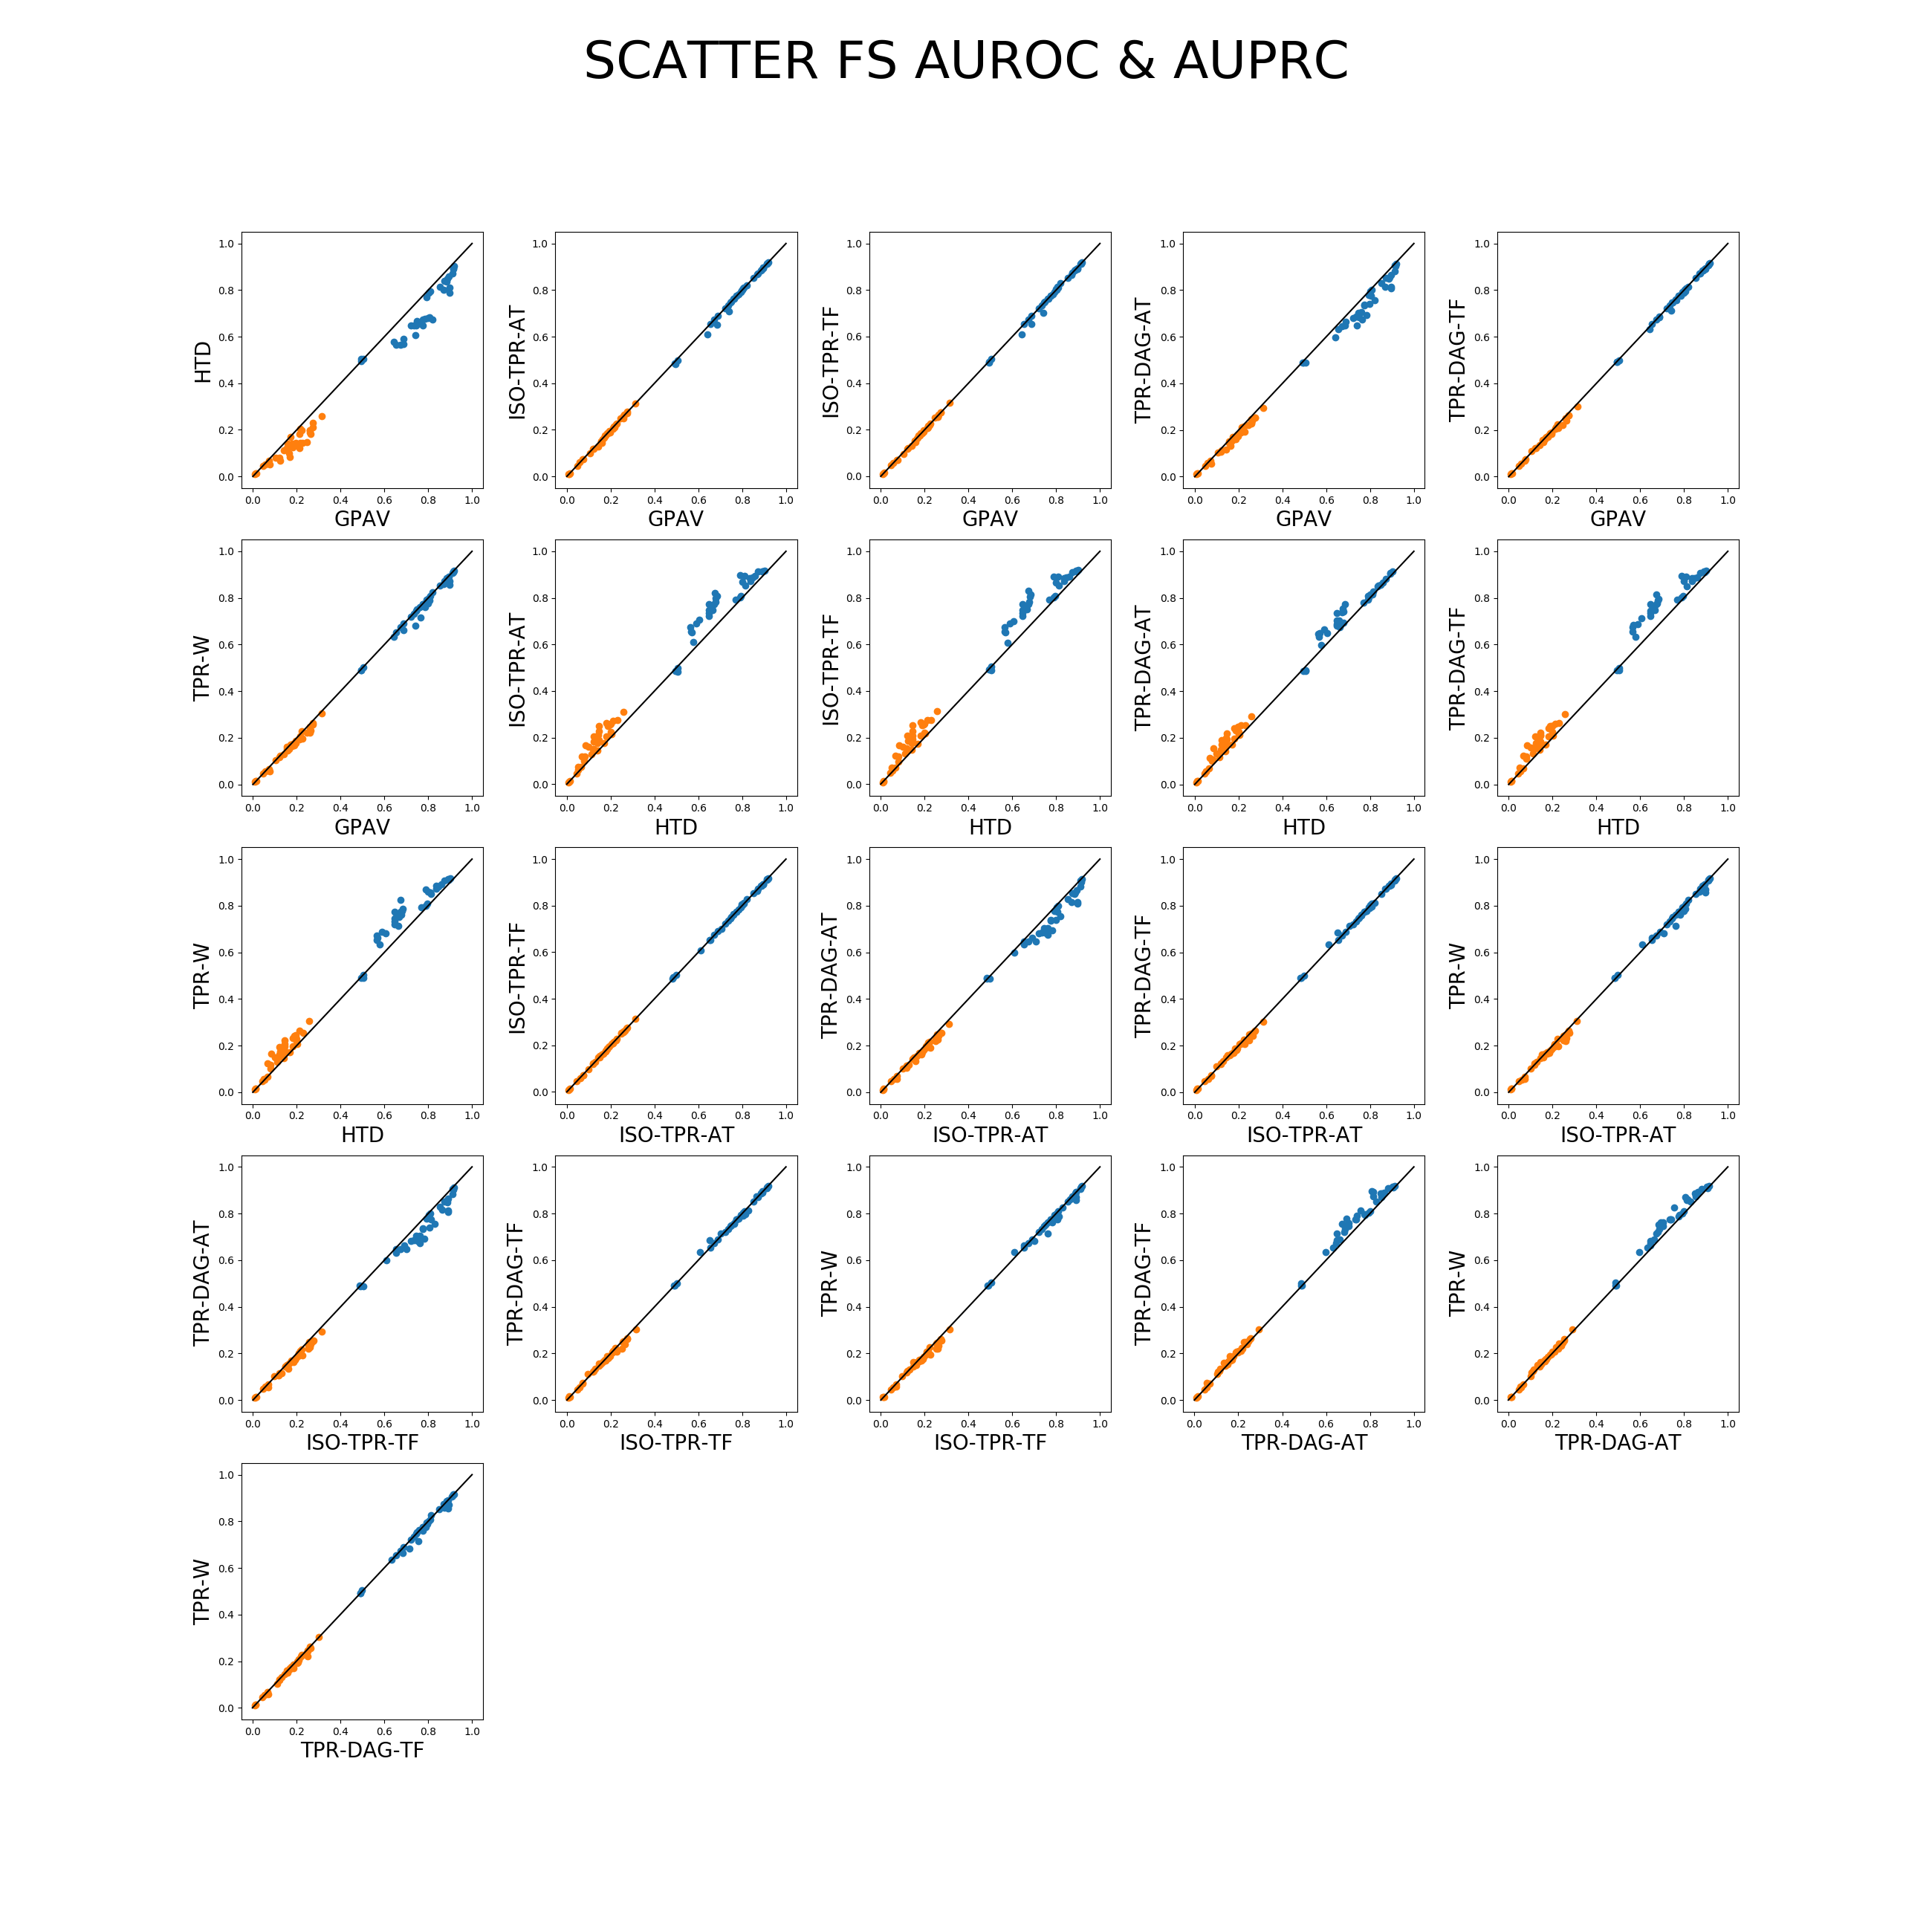
\includegraphics[scale=0.3]{./images/scatterplot_FS.png}
\caption{\footnotesize{Scatter plot del valore atteso stimato per AUROC (pallini blu) e AUPRC (pallini arancioni) a seconda del metodo di ensemble gerarchico (ascisse e ordinate), per la riduzione della dimensionalità con correlazione di Pearson e tutte e tre le ontologie (BP, MF, CC).}}
\label{scatter_1}
\end{figure}

\begin{figure}
 \hspace*{-2.6cm}
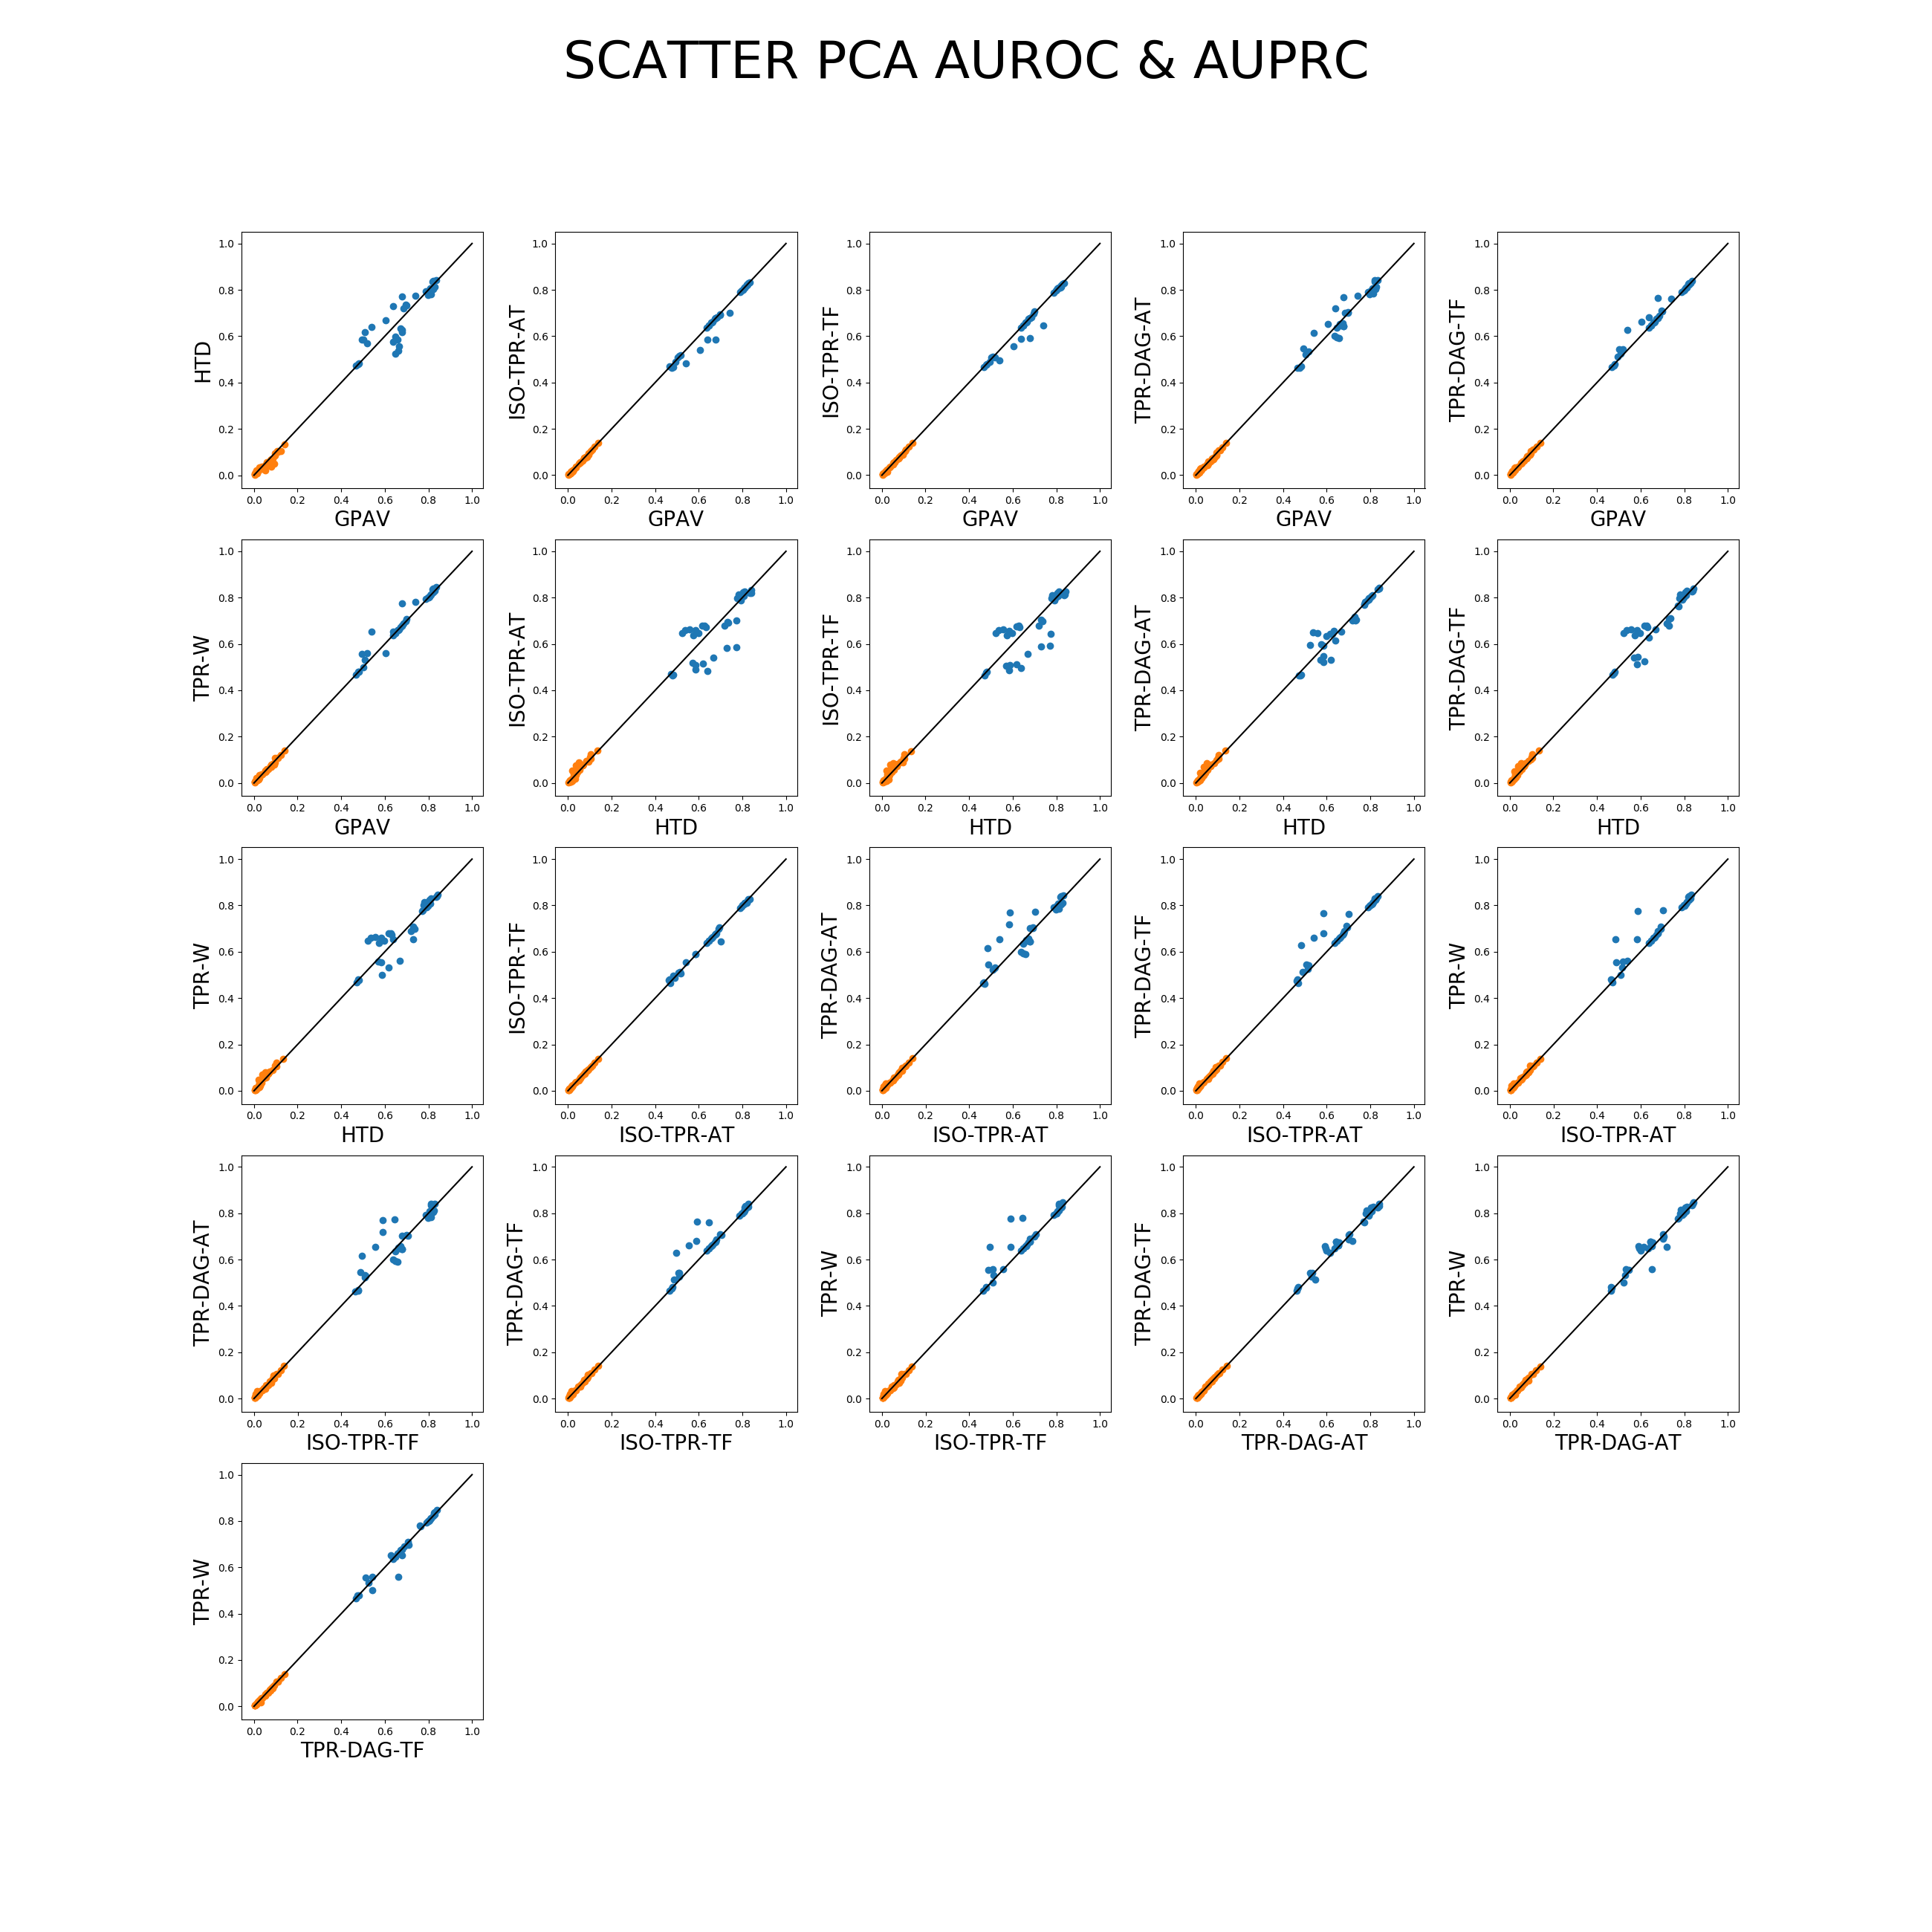
\includegraphics[scale=0.3]{./images/scatterplot_PCA.png}
\caption{\footnotesize{Scatter plot del valore atteso stimato per AUROC (pallini blu) e AUPRC (pallini arancioni) a seconda del metodo di ensemble gerarchico (ascisse e ordinate), per la riduzione della dimensionalità con PCA e tutte e tre le ontologie (BP, MF, CC).}}
\label{scatter_2}
\end{figure}


\chapter{Conclusioni}
A seguito del lavoro sperimentale si è giunti alla conclusione che i metodi ensemble gerarchici riescono ad apportare miglioramenti statisticamente significativi alle performance dei predittori flat, addestrati sulle singole classi di un output strutturato, a patto di avere delle predizioni di partenza \emph{sufficientemente} accurate. Infatti, a seguito di due diverse tipologie di riduzione della dimensionalità, e cioè selezione delle feature tramite correlazione di Pearson e selezione delle componenti con PCA, si sono osservate performance nettamente migliori per i metodi ensemble gerarchici a seguito della prima selezione, che conduce a predizioni più accurate per i predittori flat. 
\newline
\newline
Anche se in teoria le tecniche di riduzione della dimensionalità possono essere utilizzate per portare a sensibili miglioramenti delle performance di un predittore, l'introduzione di queste due tipologie di selezione delle feature si è resa necessaria principalmente a causa dei tempi di calcolo eccessivamente lunghi per l'addestramento dei classificatori flat. La selezione delle feature con correlazione di Pearson richiede tempi decisamente più lunghi della selezione con PCA, ma determina un vantaggio statisticamente significativo a livello di performance rispetto a quest'ultima.
\newline
\newline
Anche il tuning degli algoritmi di machine learning di partenza svolge un ruolo importante per il successo dei metodi ensemble gerarchici. Infatti, a parità di selezione delle feature (PCA o FS), alcuni algoritmi hanno prodotto predittori flat scadenti, che non hanno consentito ai metodi di ensemble gerarchici di migliorare le performance. È il caso ad esempio dell'algoritmo \emph{glmnet}, che, senza un'adeguata configurazione, ha prodotto risultati vicini a quelli di un predittore casuale, che in fase di correzione gerarchica hanno portato a risultati scadenti.
\newline
\newline
I nuovi metodi ensemble gerarchici introdotti in questa tesi, e cioè quelli basati sulla \emph{Isotonic Regression}, si sono dimostrati competitivi rispetto ai metodi  ensemble gerarchici allo stato dell'arte, e in alcuni contesti (selezione delle feature con correlazione di Pearson) hanno prodotto risultati significativamente migliori rispetto agli algoritmi allo stato dell'arte.

Alcune future linee di ricerca che si potrebbero perseguire per valutare più approfonditamente e migliorare le prestazioni dei metodi di ensemble gerarchici, sono le seguenti:

\begin{itemize}
\item Ampliare il numero di specie su cui effettuare l'analisi.
\item Effettuare un tuning più accurato degli algoritmi di machine learning selezionati, tenendo in considerazione che le classi dell'output strutturato sono spesso sbilanciate all'interno dei dataset per la GO.
\item Introdurre nuove tecniche di riduzione della dimensionalità, sia per ridurre i tempi di calcolo (complessità) che per migliorare i risultati dei classificatori base (performance).
\item Utilizzare altre tipologie di selezione dei figli per lo step bottom-up della True Path Rule, in combinazione e non (a esempio effettuando una selezione dei figli pesata con soglia adattiva).
\item Analizzare in maniera più approfondita le performance, ad esempio in relazione ad altre metriche, come la F-score gerarchica.
\item Confrontare i metodi ensemble con i diversi metodi per la predizione su output strutturati, come ad esempio i metodi Kernel o i metodi basati su reti.
\end{itemize} 

%			BIBLIOGRAFIA
%
\begin{appendices}
\chapter{Codice}
\lstinputlisting[language=R, caption=\footnotesize{Le configurazioni di default utilizzate per i diversi algoritmi di apprendimento}, label=configs]{./code/default_config2.R}

\newpage
\lstinputlisting[language=R, caption=\footnotesize{Script di esempio per il train e test dei metodi flat con cross-validation}, label=exampleTrainR]{./code/snippet.R}
\chapter{Boxplot}
\begin{figure}[h]
 \hspace*{-2.6cm}
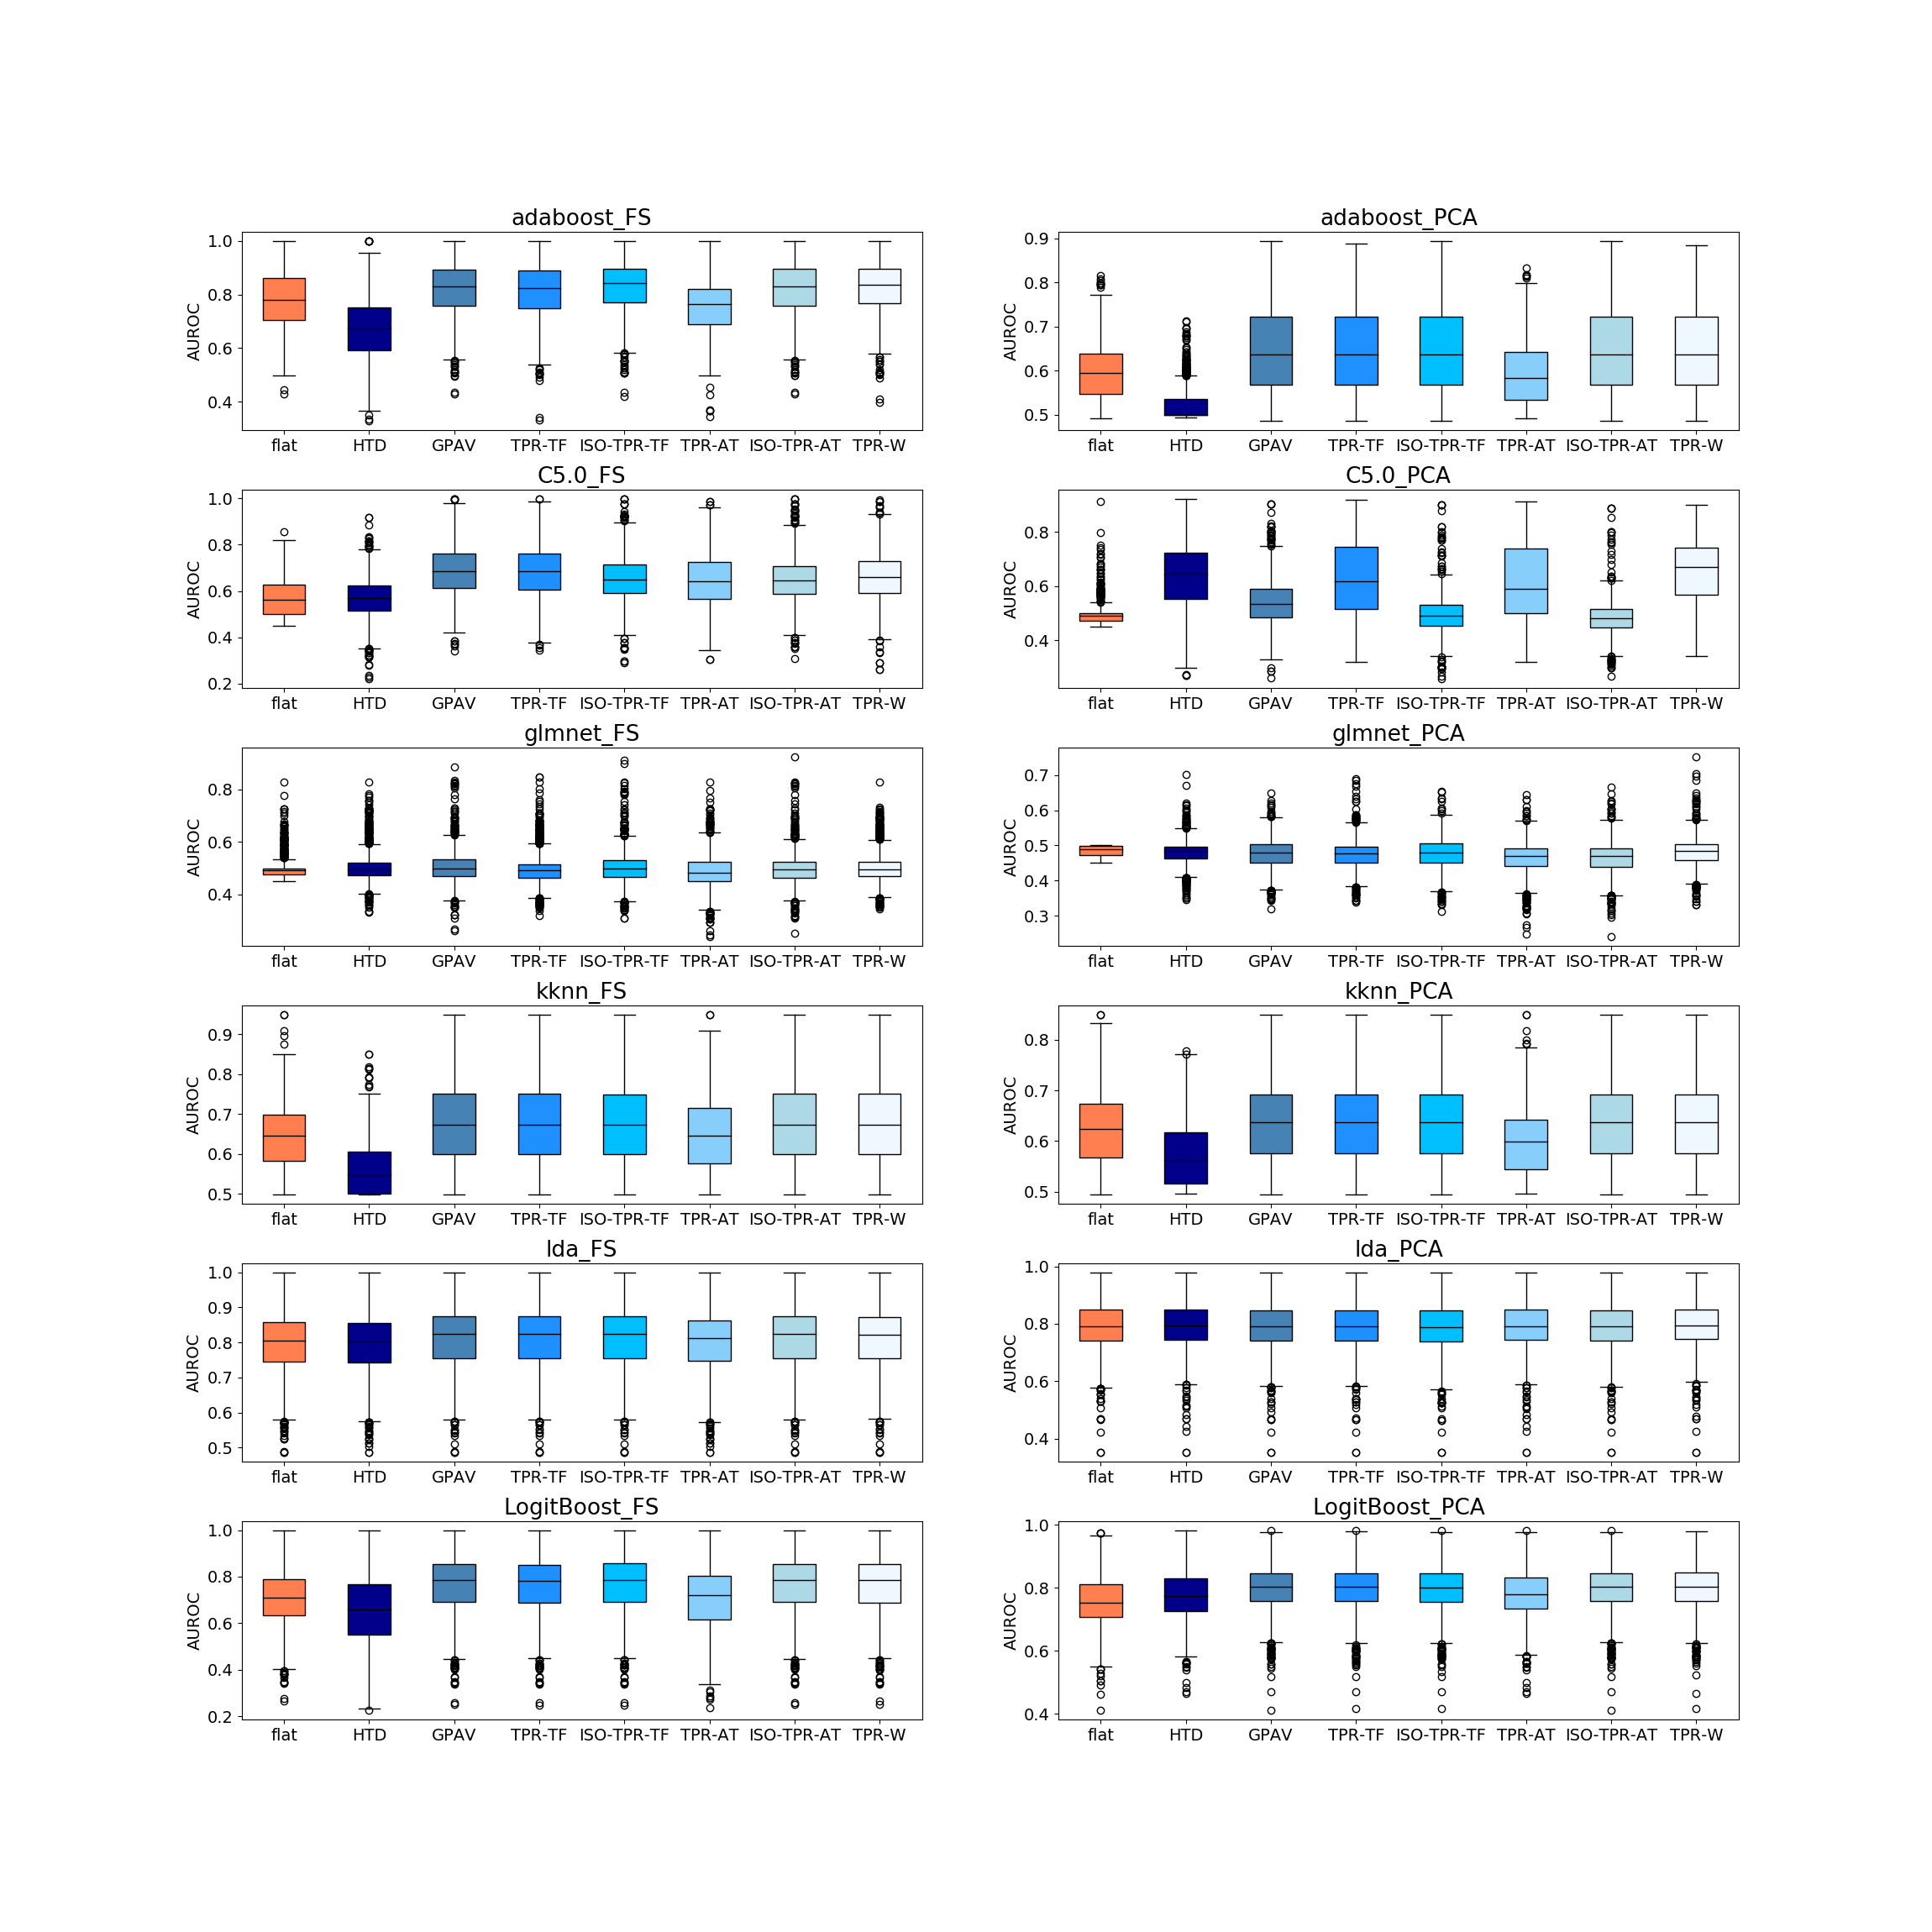
\includegraphics[scale=0.34]{./images/BP_AUC_1.png}
\caption{\footnotesize{Boxplot per l'ontologia BP, relativi alla metrica AUROC al variare di: metodi gerarchici utilizzati, algoritmi di ML (primi 6) e metodo di riduzione della dimensionalità.}}
\label{BP_AUC_1}
\end{figure}


\begin{figure}[h]
 \hspace*{-2.6cm}
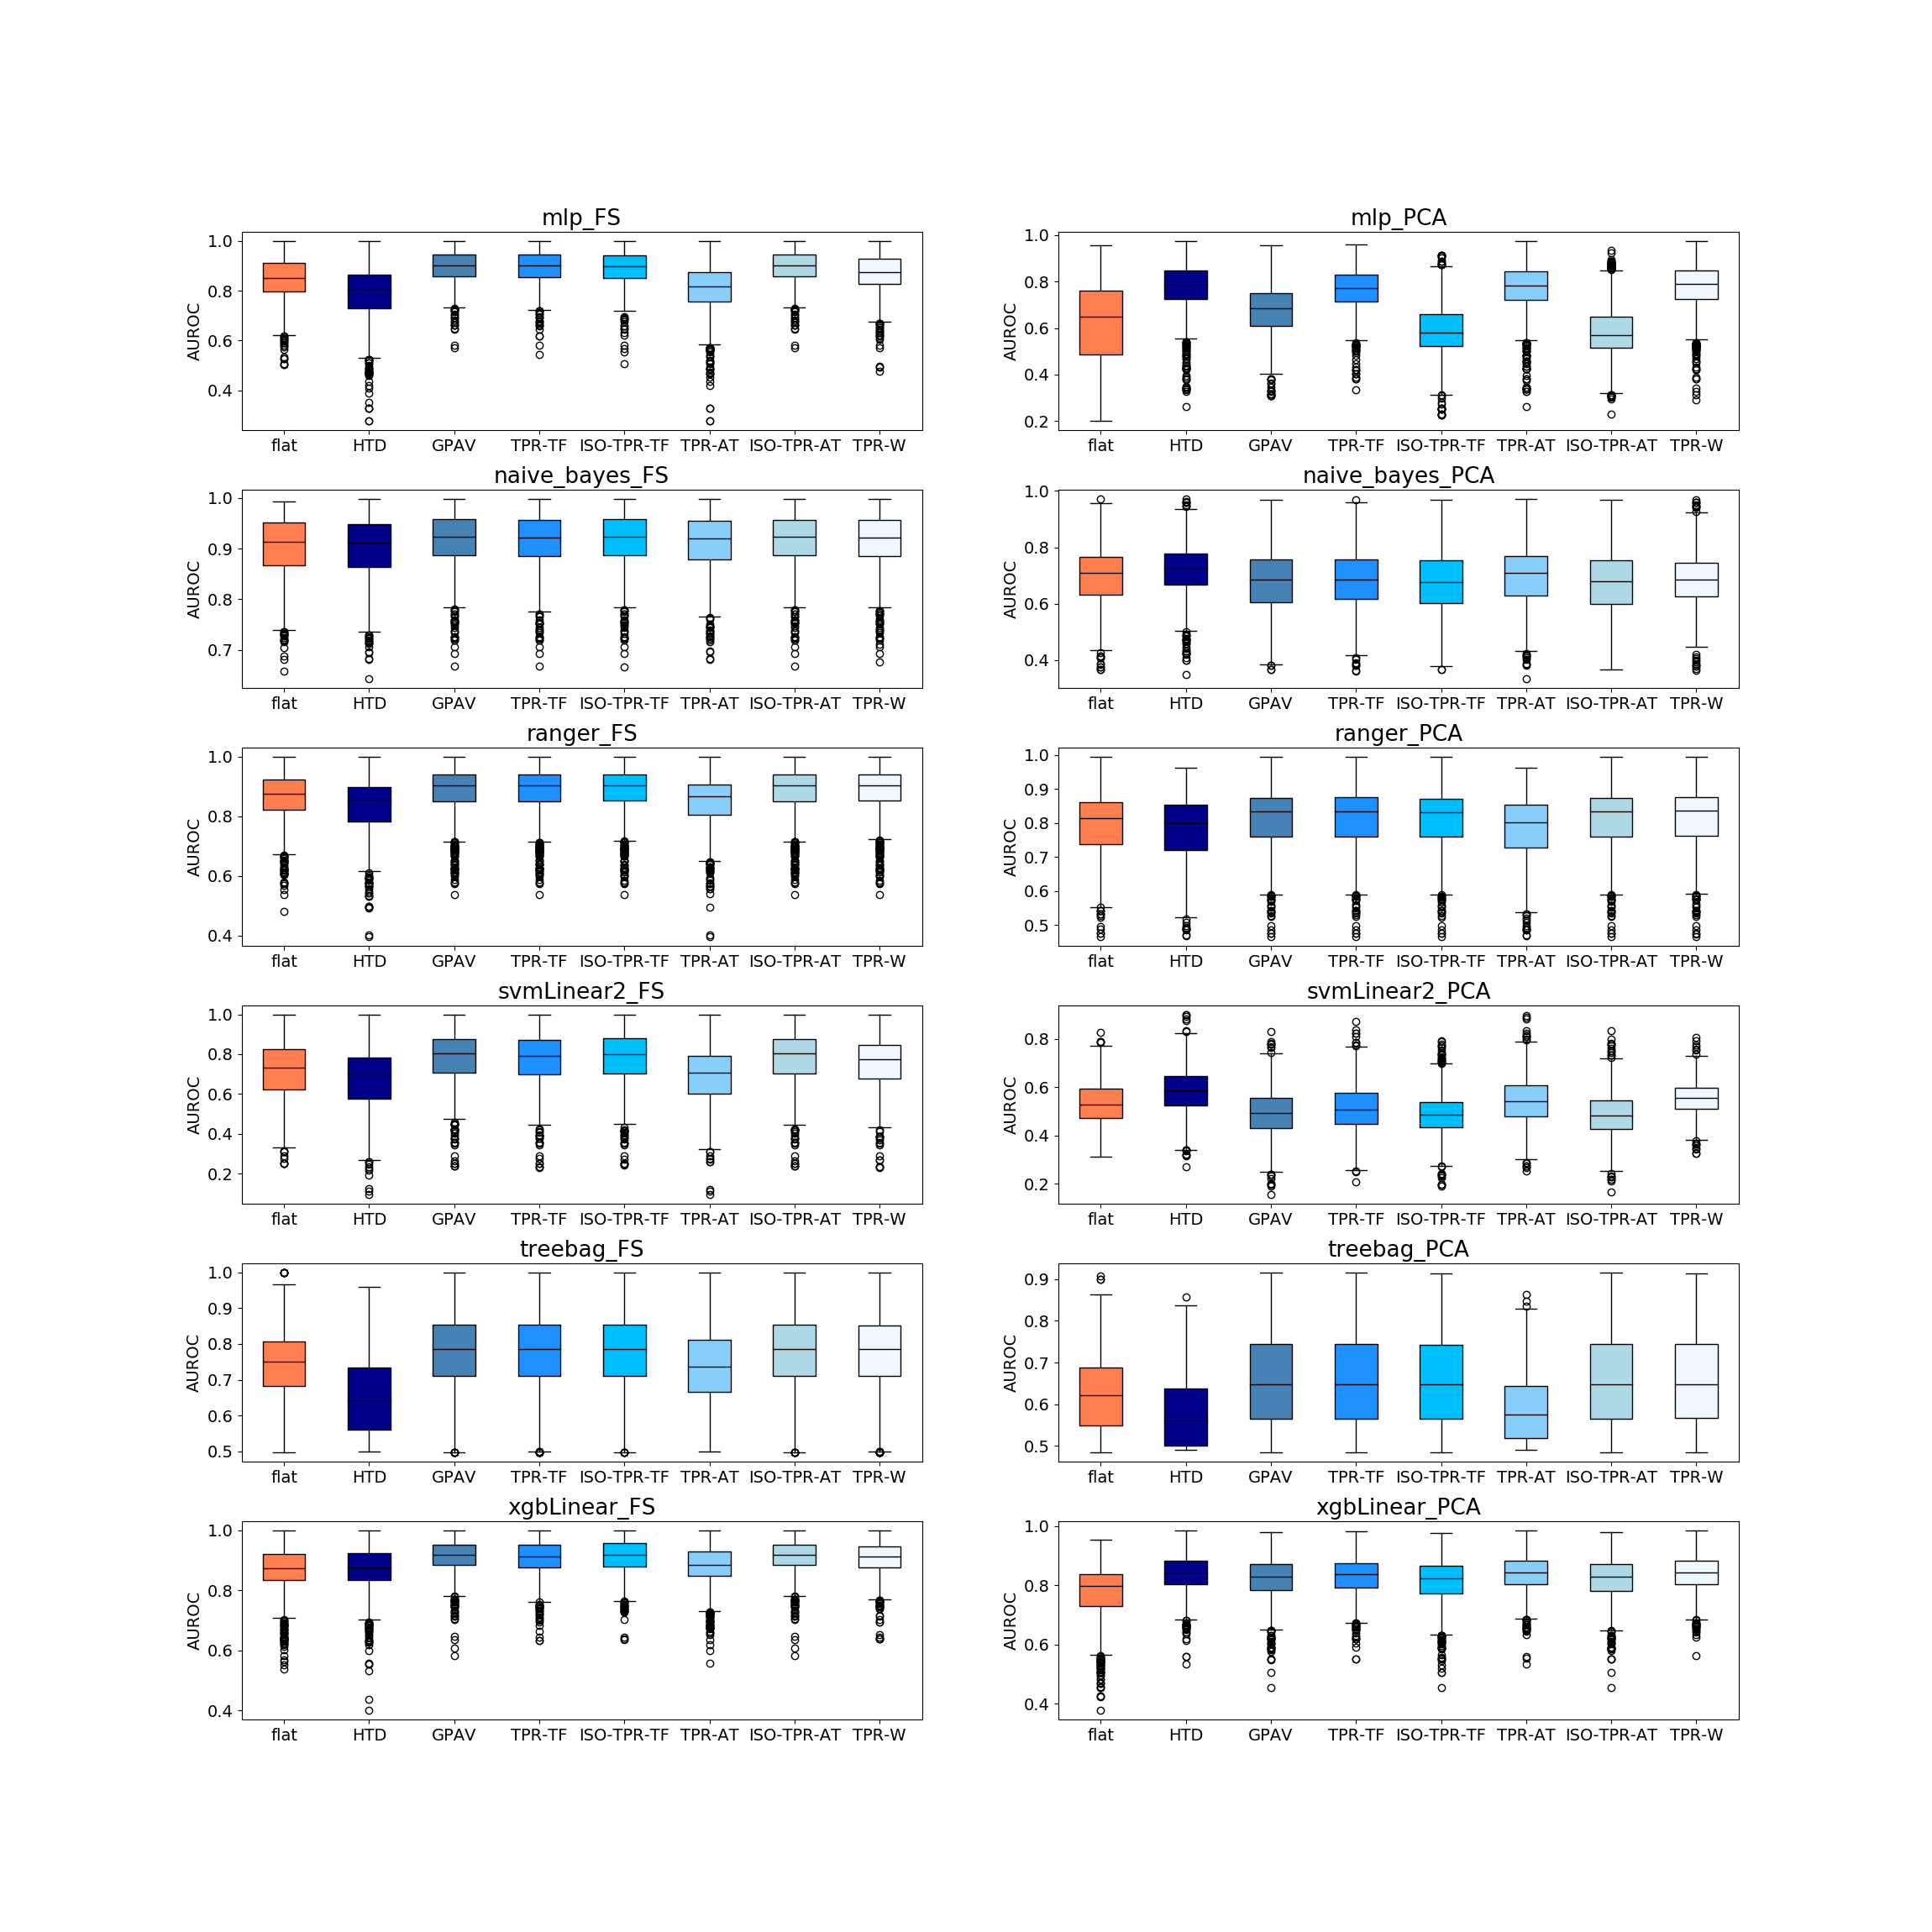
\includegraphics[scale=0.34]{./images/BP_AUC_2.png}
\caption{\footnotesize{Boxplot per l'ontologia BP, relativi alla metrica AUROC al variare di: metodi gerarchici utilizzati, algoritmi di ML (ultimi 6) e metodo di riduzione della dimensionalità.}}
\label{BP_AUC_2}
\end{figure}

\begin{figure}[h]
 \hspace*{-2.6cm}
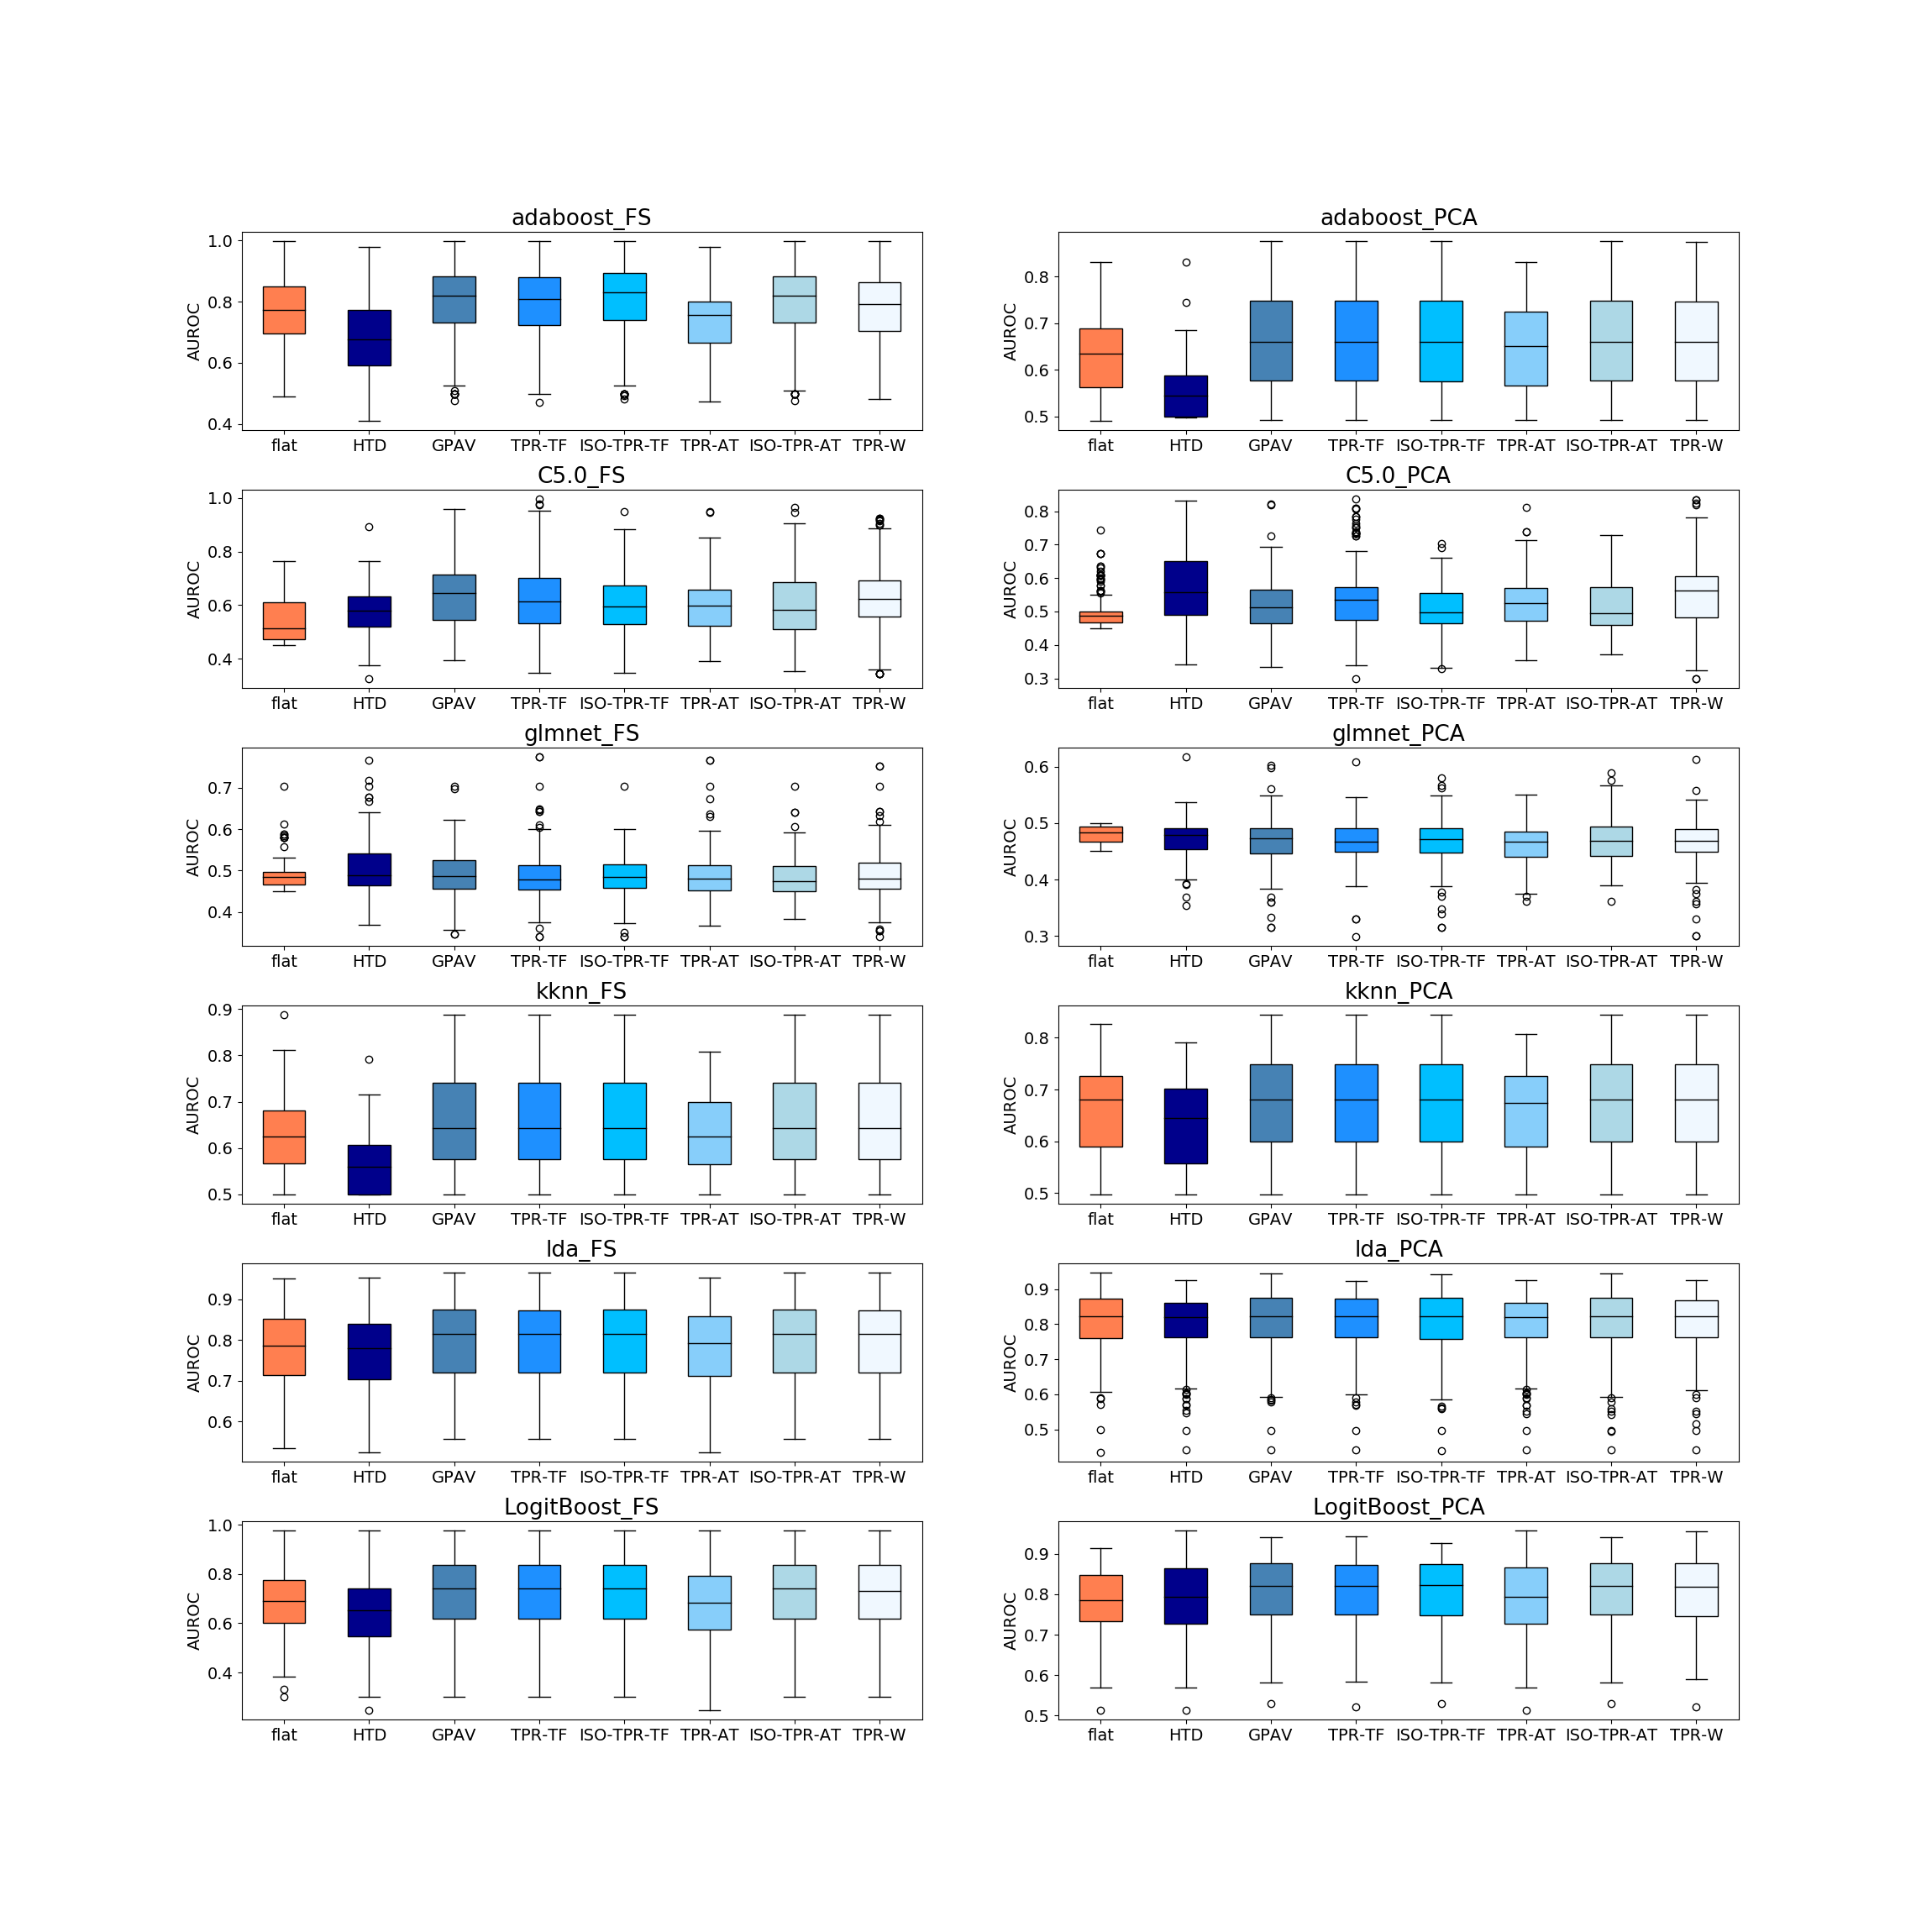
\includegraphics[scale=0.34]{./images/MF_AUC_1.png}
\caption{\footnotesize{Boxplot per l'ontologia MF, relativi alla metrica AUROC al variare di: metodi gerarchici utilizzati, algoritmi di ML (primi 6) e metodo di riduzione della dimensionalità.}}
\label{MF_AUC_1}
\end{figure}

\begin{figure}[h]
 \hspace*{-2.6cm}
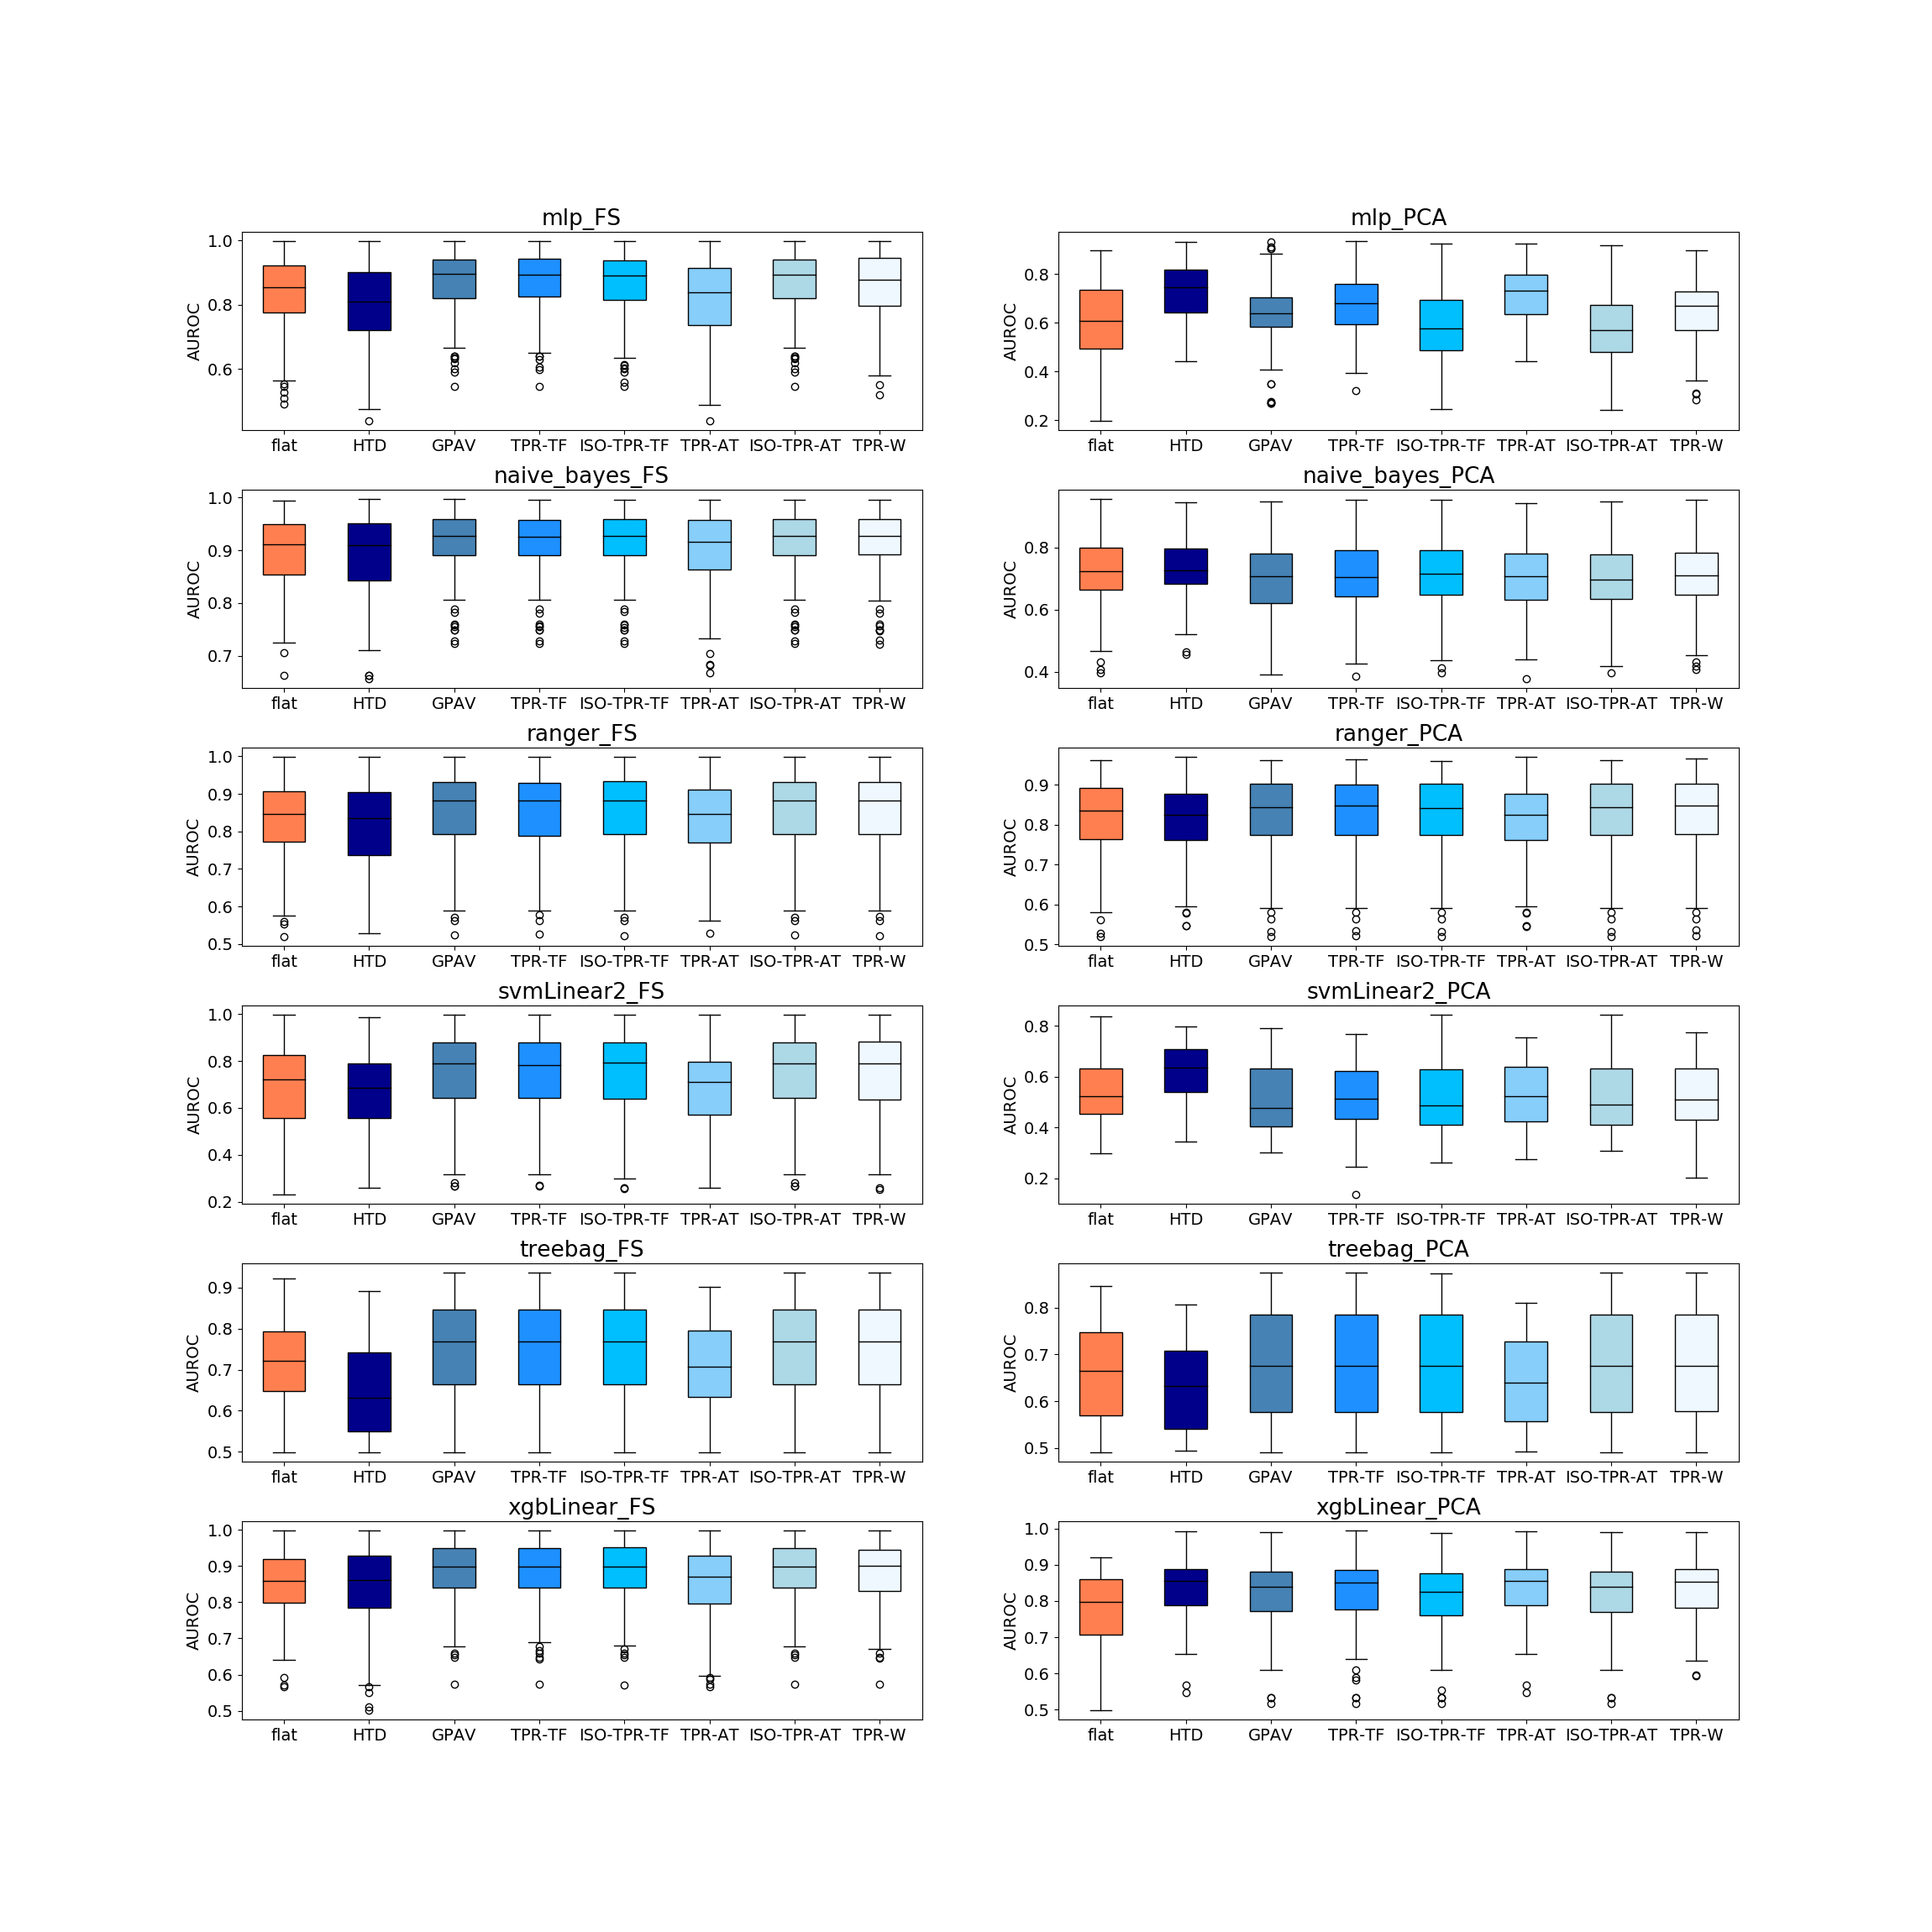
\includegraphics[scale=0.34]{./images/MF_AUC_2.png}
\caption{\footnotesize{Boxplot per l'ontologia MF, relativi alla metrica AUROC al variare di: metodi gerarchici utilizzati, algoritmi di ML (ultimi 6) e metodo di riduzione della dimensionalità.}}
\label{MF_AUC_2}
\end{figure}

\begin{figure}[h]
 \hspace*{-2.6cm}
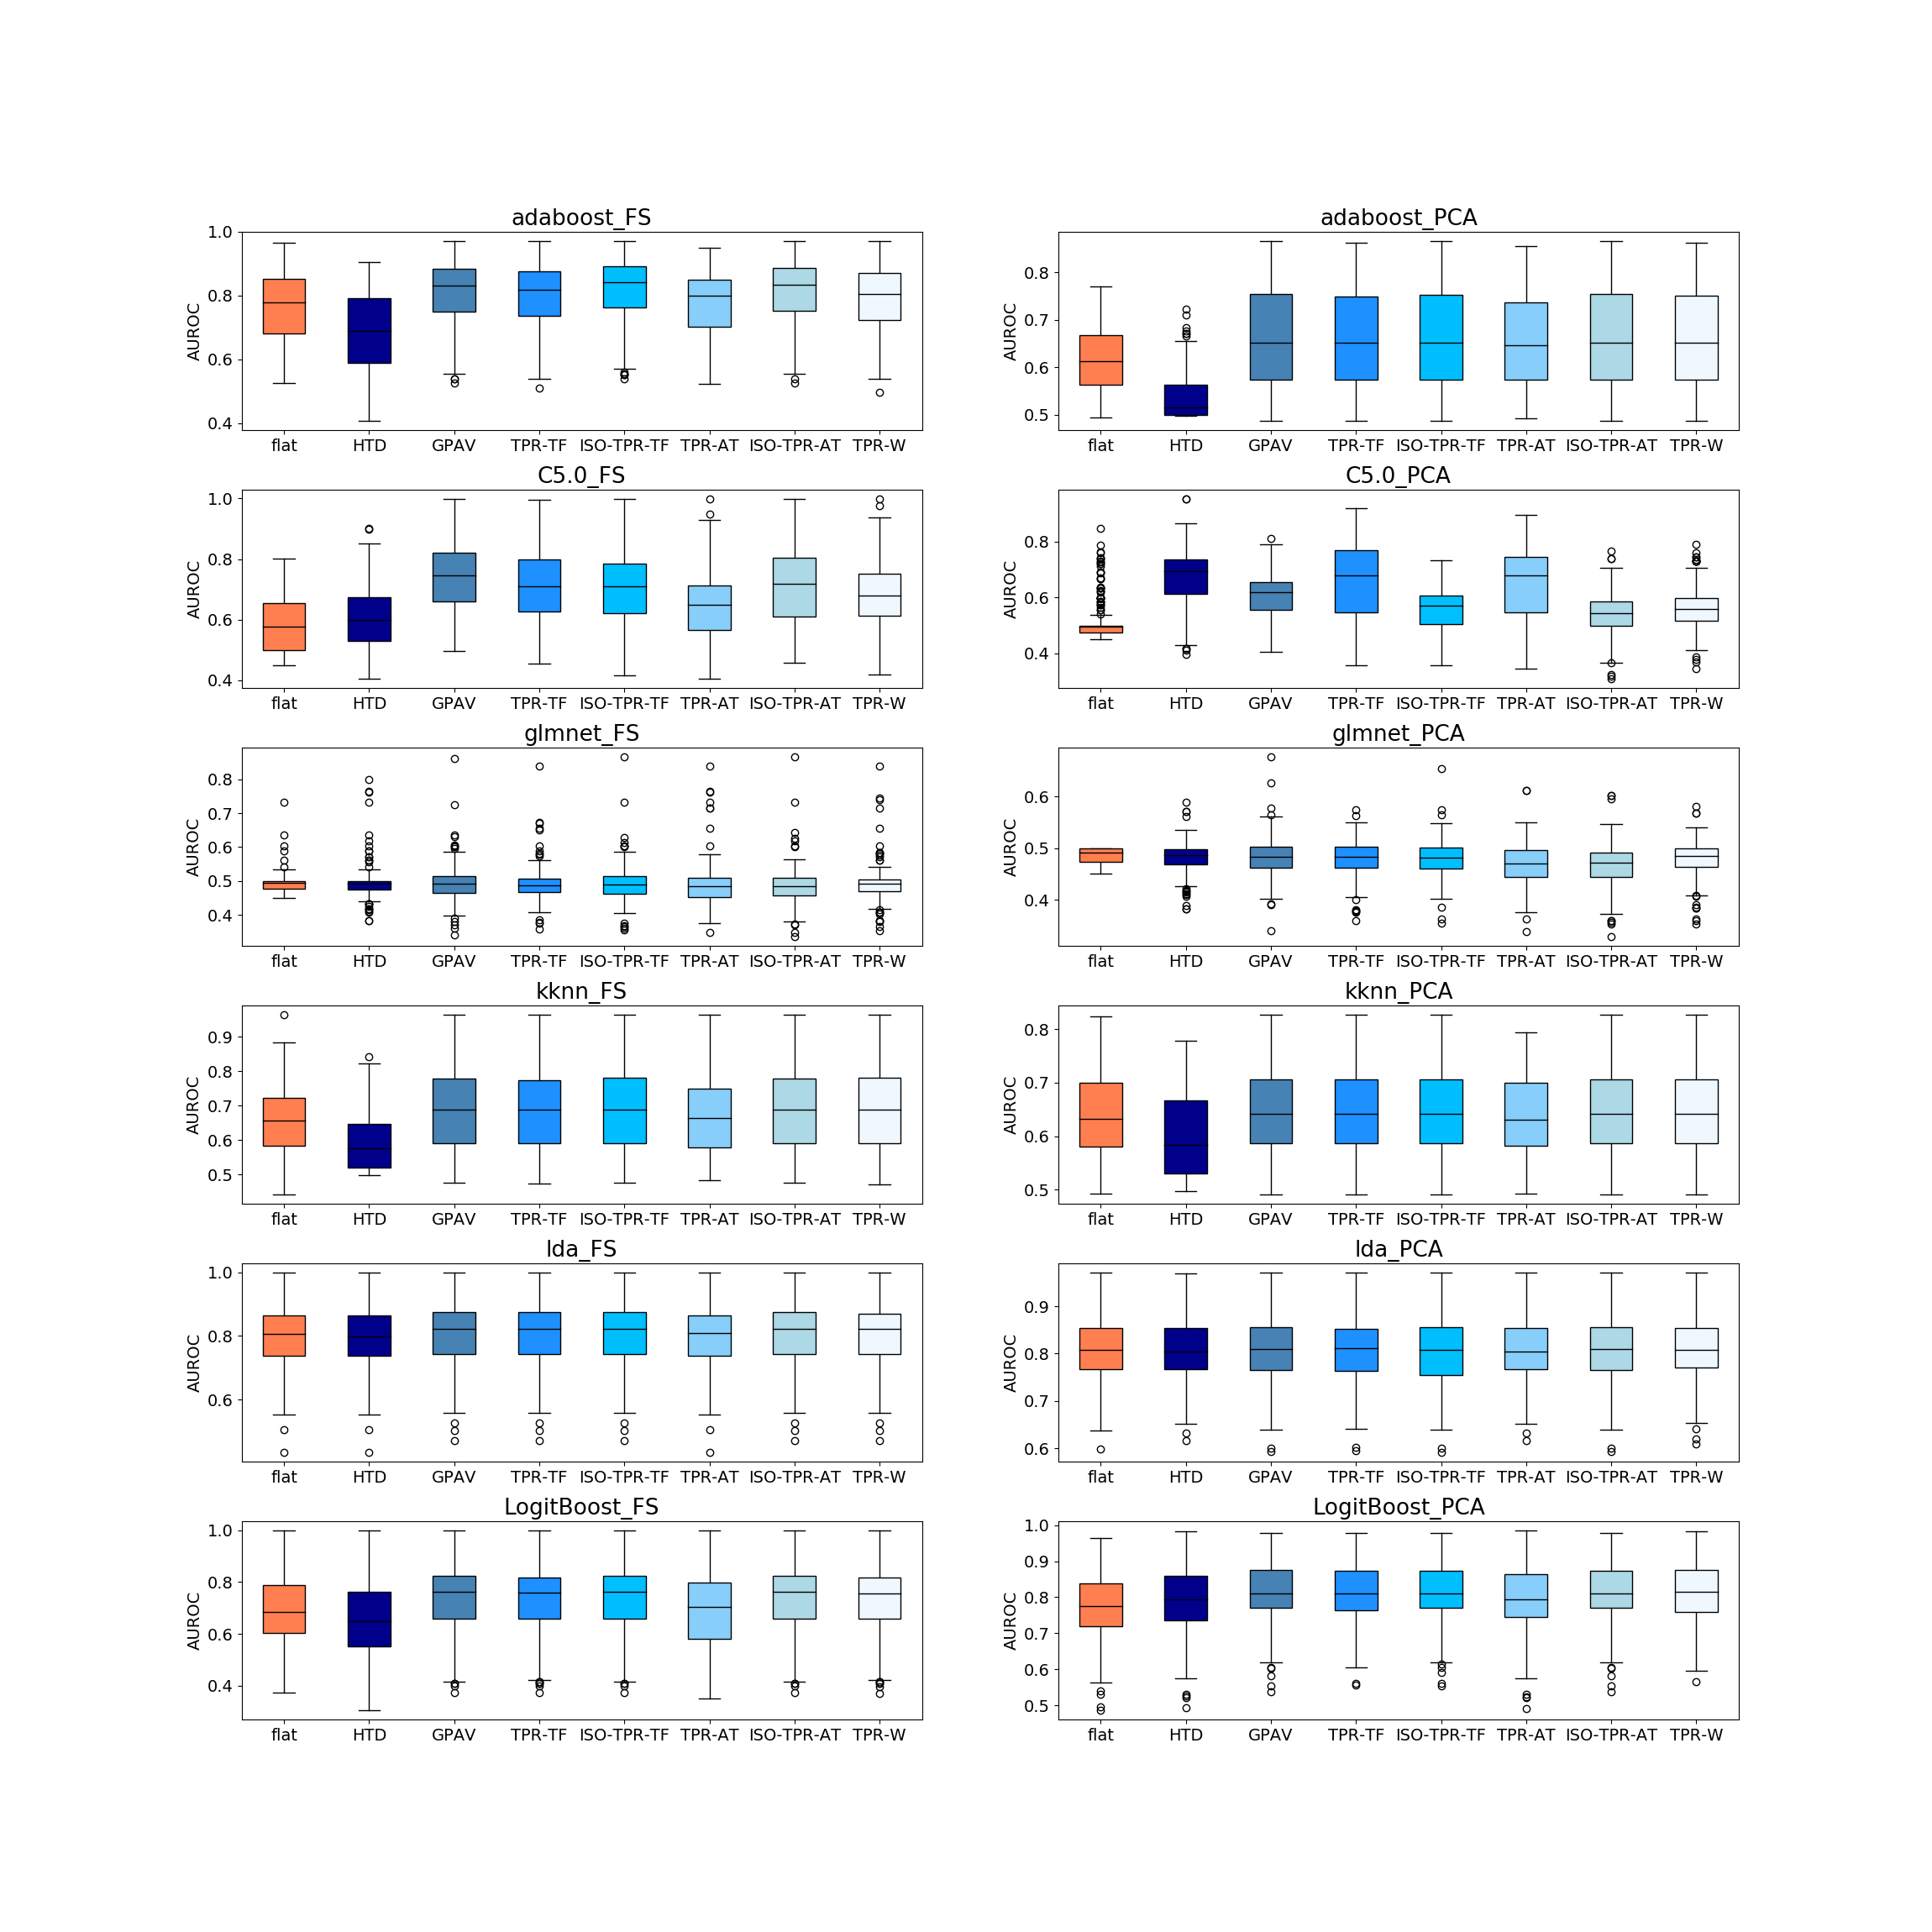
\includegraphics[scale=0.34]{./images/CC_AUC_1.png}
\caption{\footnotesize{Boxplot per l'ontologia CC, relativi alla metrica AUROC al variare di: metodi gerarchici utilizzati, algoritmi di ML (primi 6) e metodo di riduzione della dimensionalità.}}
\label{CC_AUC_1}
\end{figure}

\begin{figure}[h]
 \hspace*{-2.6cm}
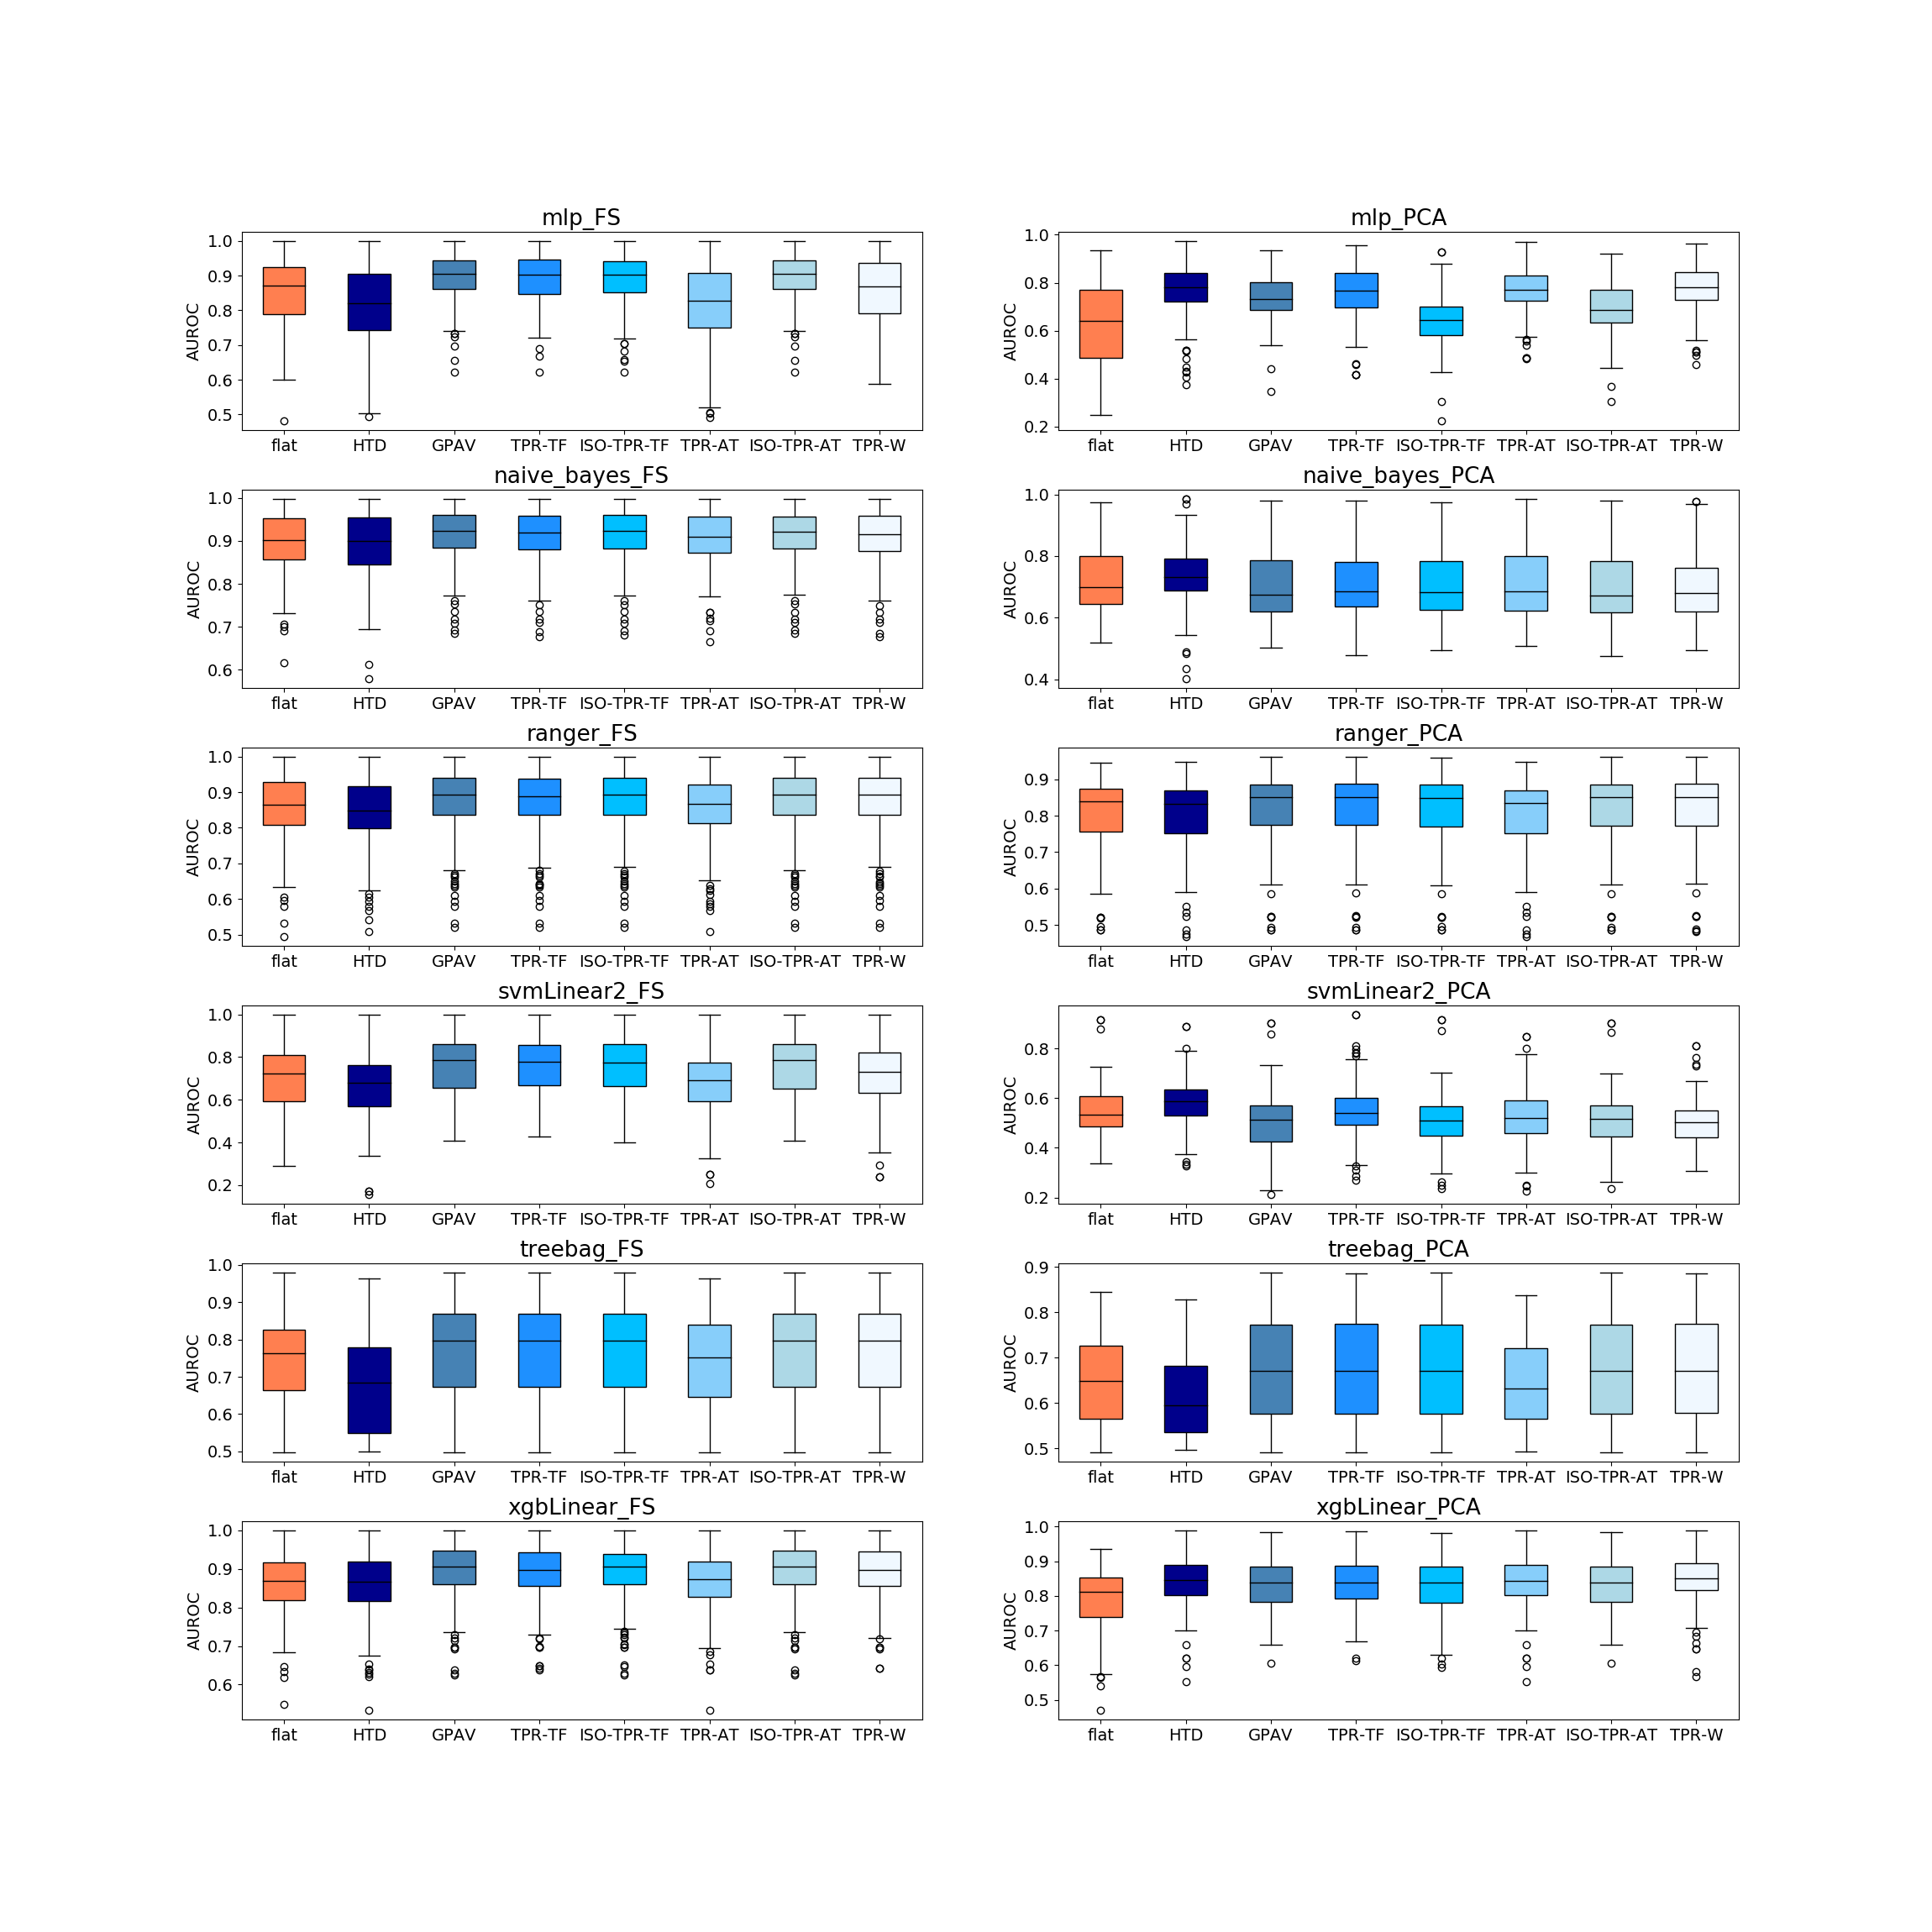
\includegraphics[scale=0.34]{./images/CC_AUC_2.png}
\caption{\footnotesize{Boxplot per l'ontologia CC, relativi alla metrica AUROC al variare di: metodi gerarchici utilizzati, algoritmi di ML (ultimi 6) e metodo di riduzione della dimensionalità.}}
\label{CC_AUC_2}
\end{figure}

\begin{figure}[h]
 \hspace*{-2.6cm}
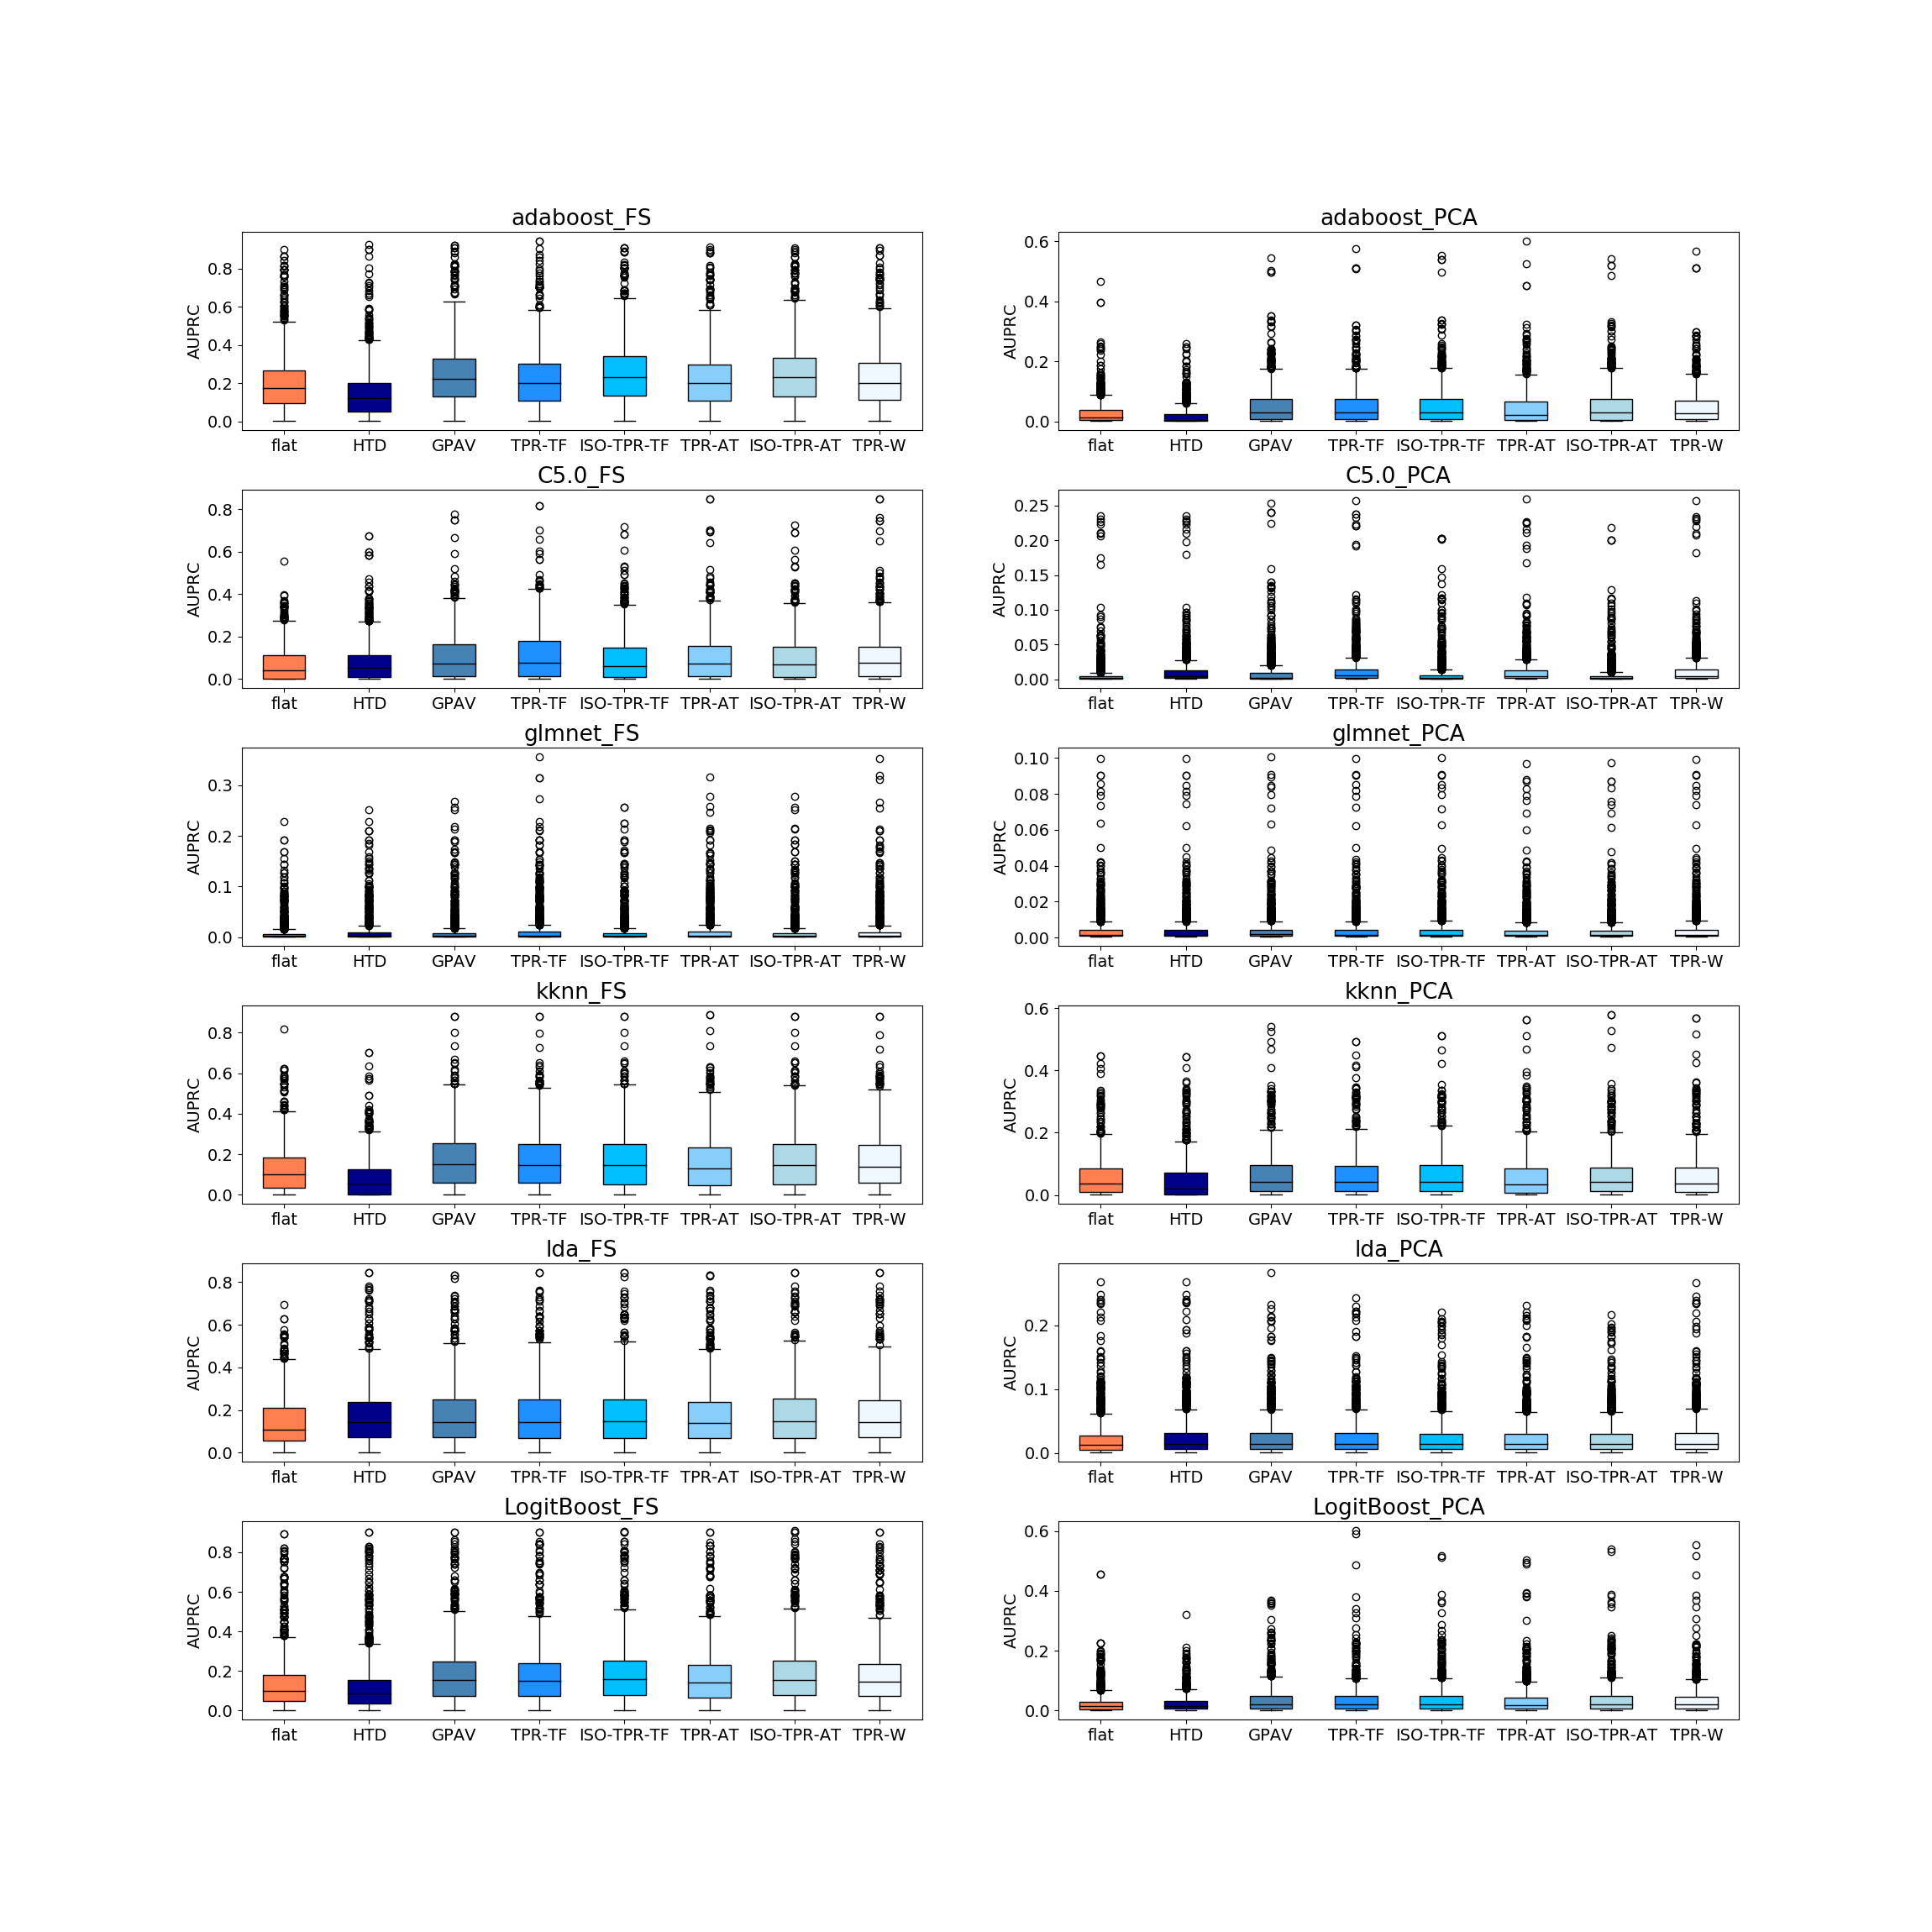
\includegraphics[scale=0.34]{./images/BP_PRC_1.png}
\caption{\footnotesize{Boxplot per l'ontologia BP, relativi alla metrica AUPRC al variare di: metodi gerarchici utilizzati, algoritmi di ML (primi 6) e metodo di riduzione della dimensionalità.}}
\label{BP_PRC_1}
\end{figure}


\begin{figure}[h]
 \hspace*{-2.6cm}
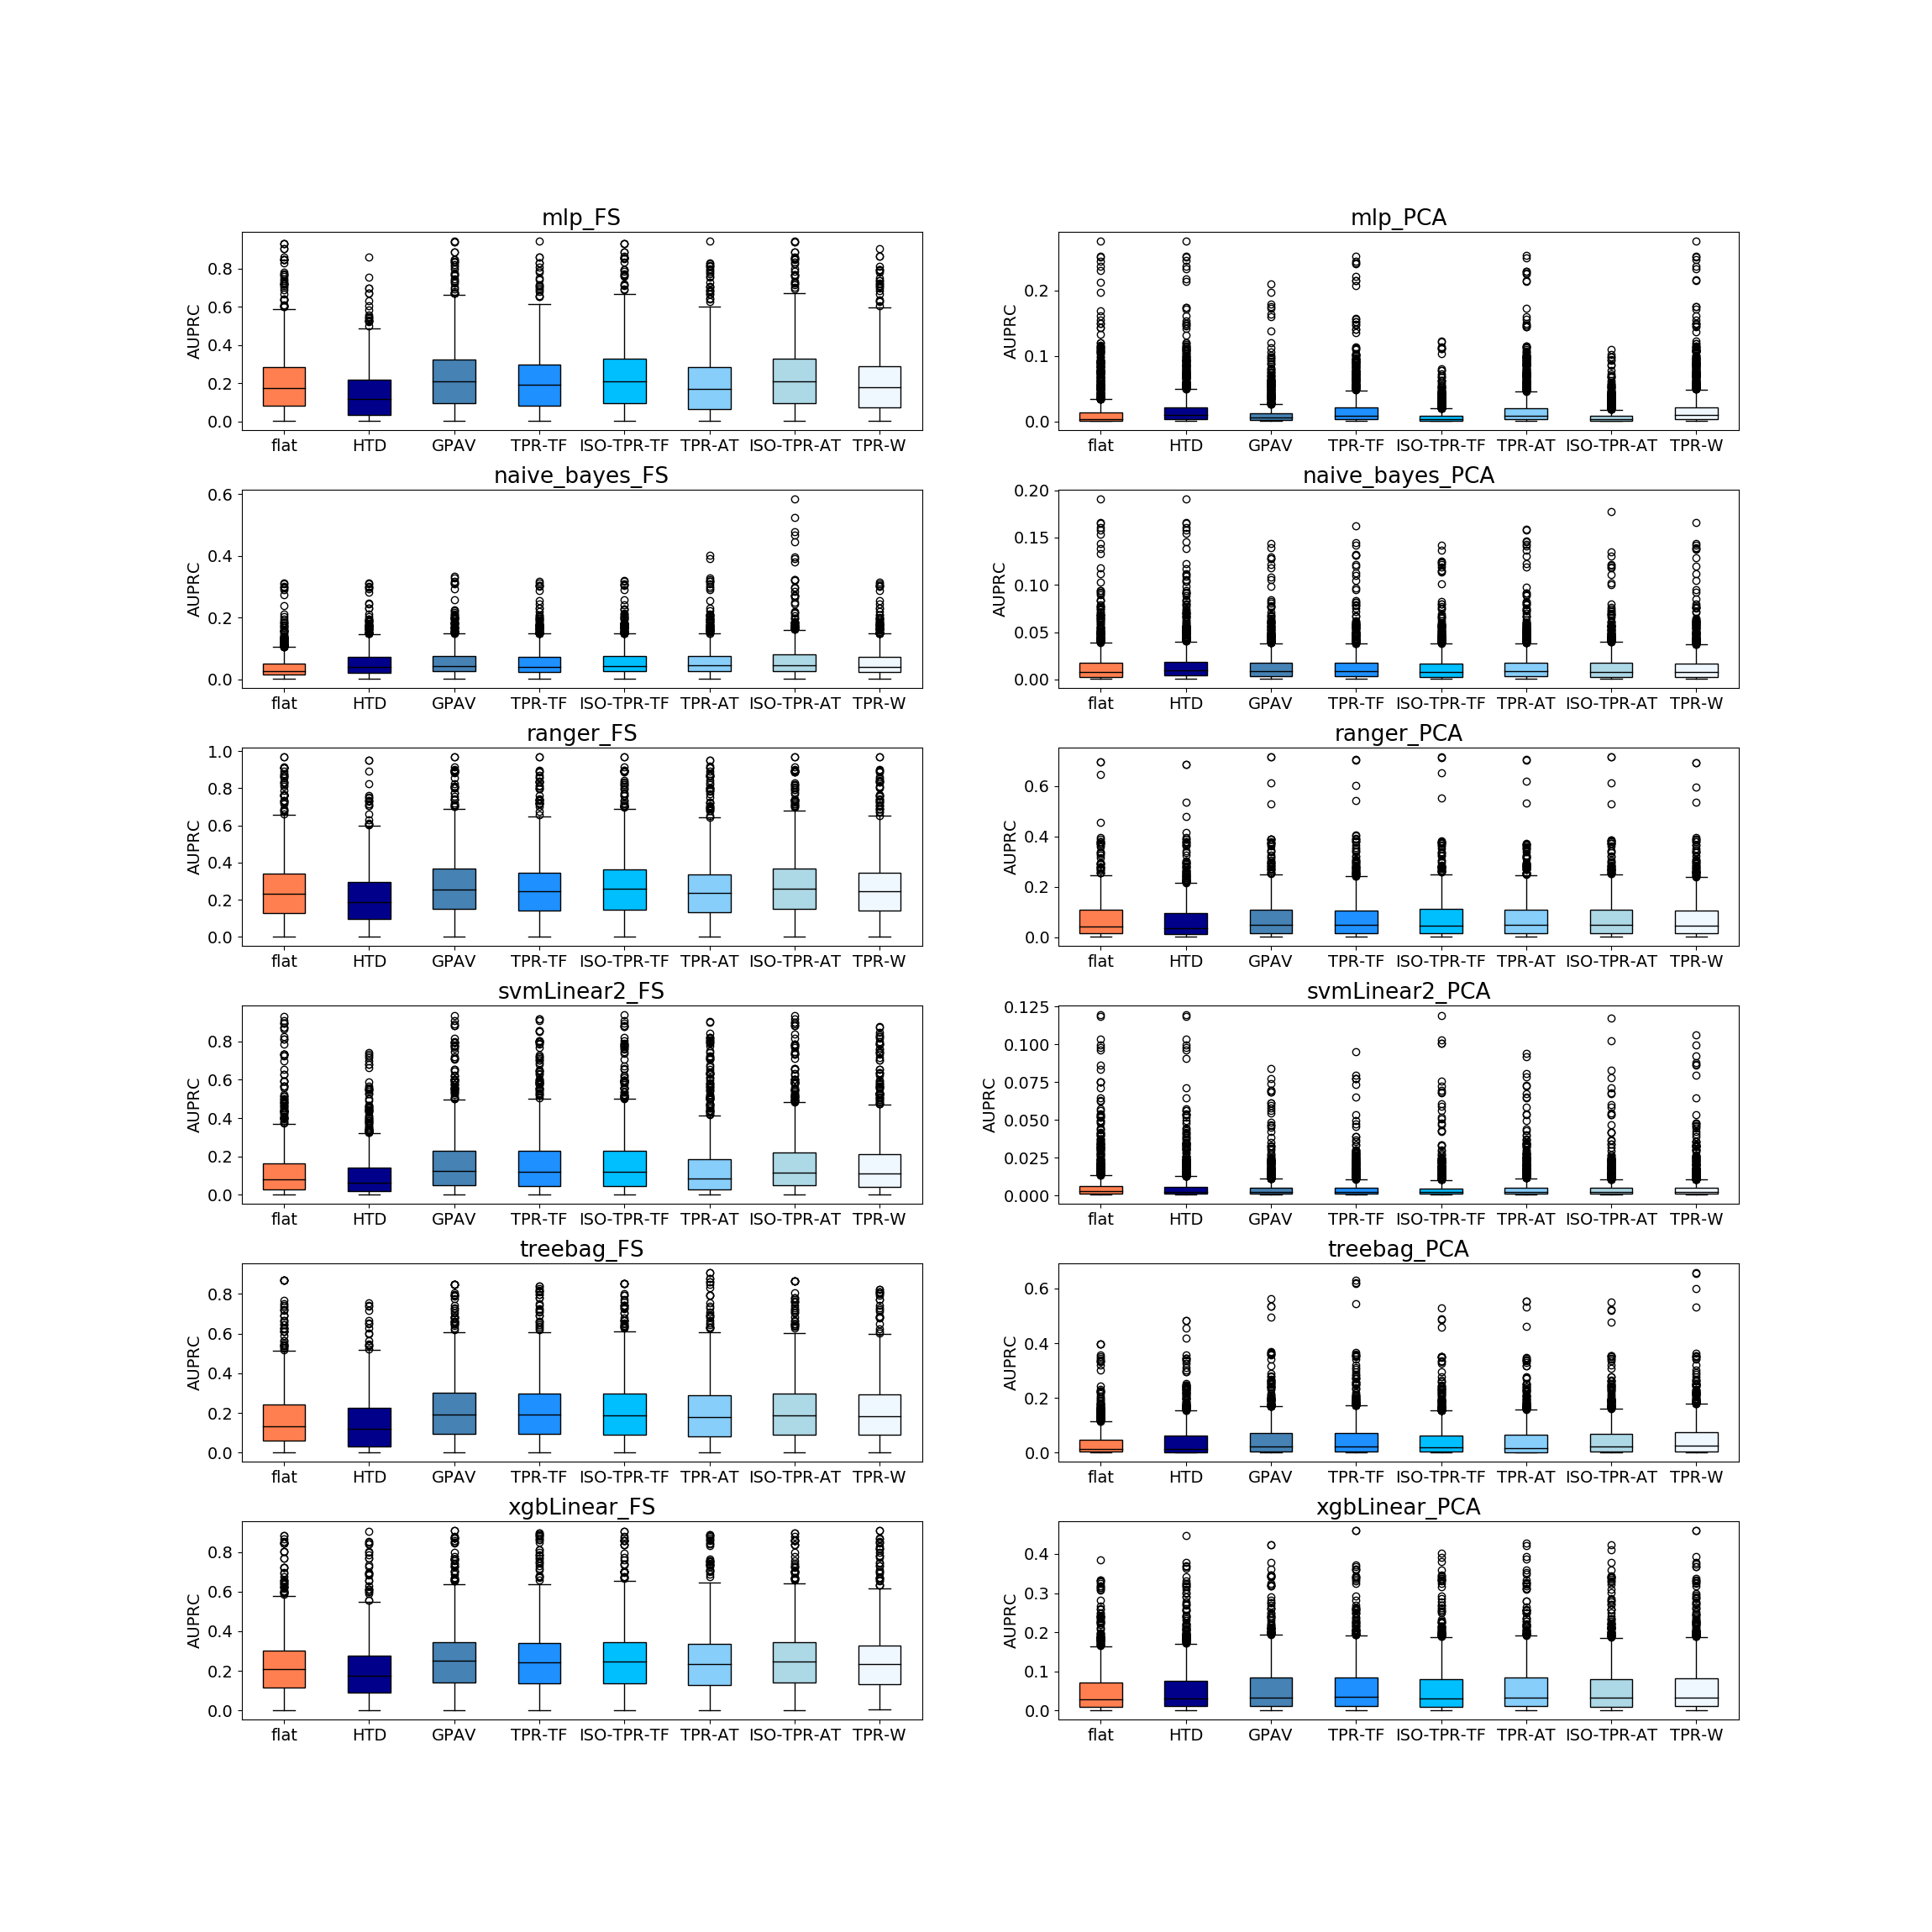
\includegraphics[scale=0.34]{./images/BP_PRC_2.png}
\caption{\footnotesize{Boxplot per l'ontologia BP, relativi alla metrica AUPRC al variare di: metodi gerarchici utilizzati, algoritmi di ML (ultimi 6) e metodo di riduzione della dimensionalità.}}
\label{BP_PRC_2}
\end{figure}

\begin{figure}[h]
 \hspace*{-2.6cm}
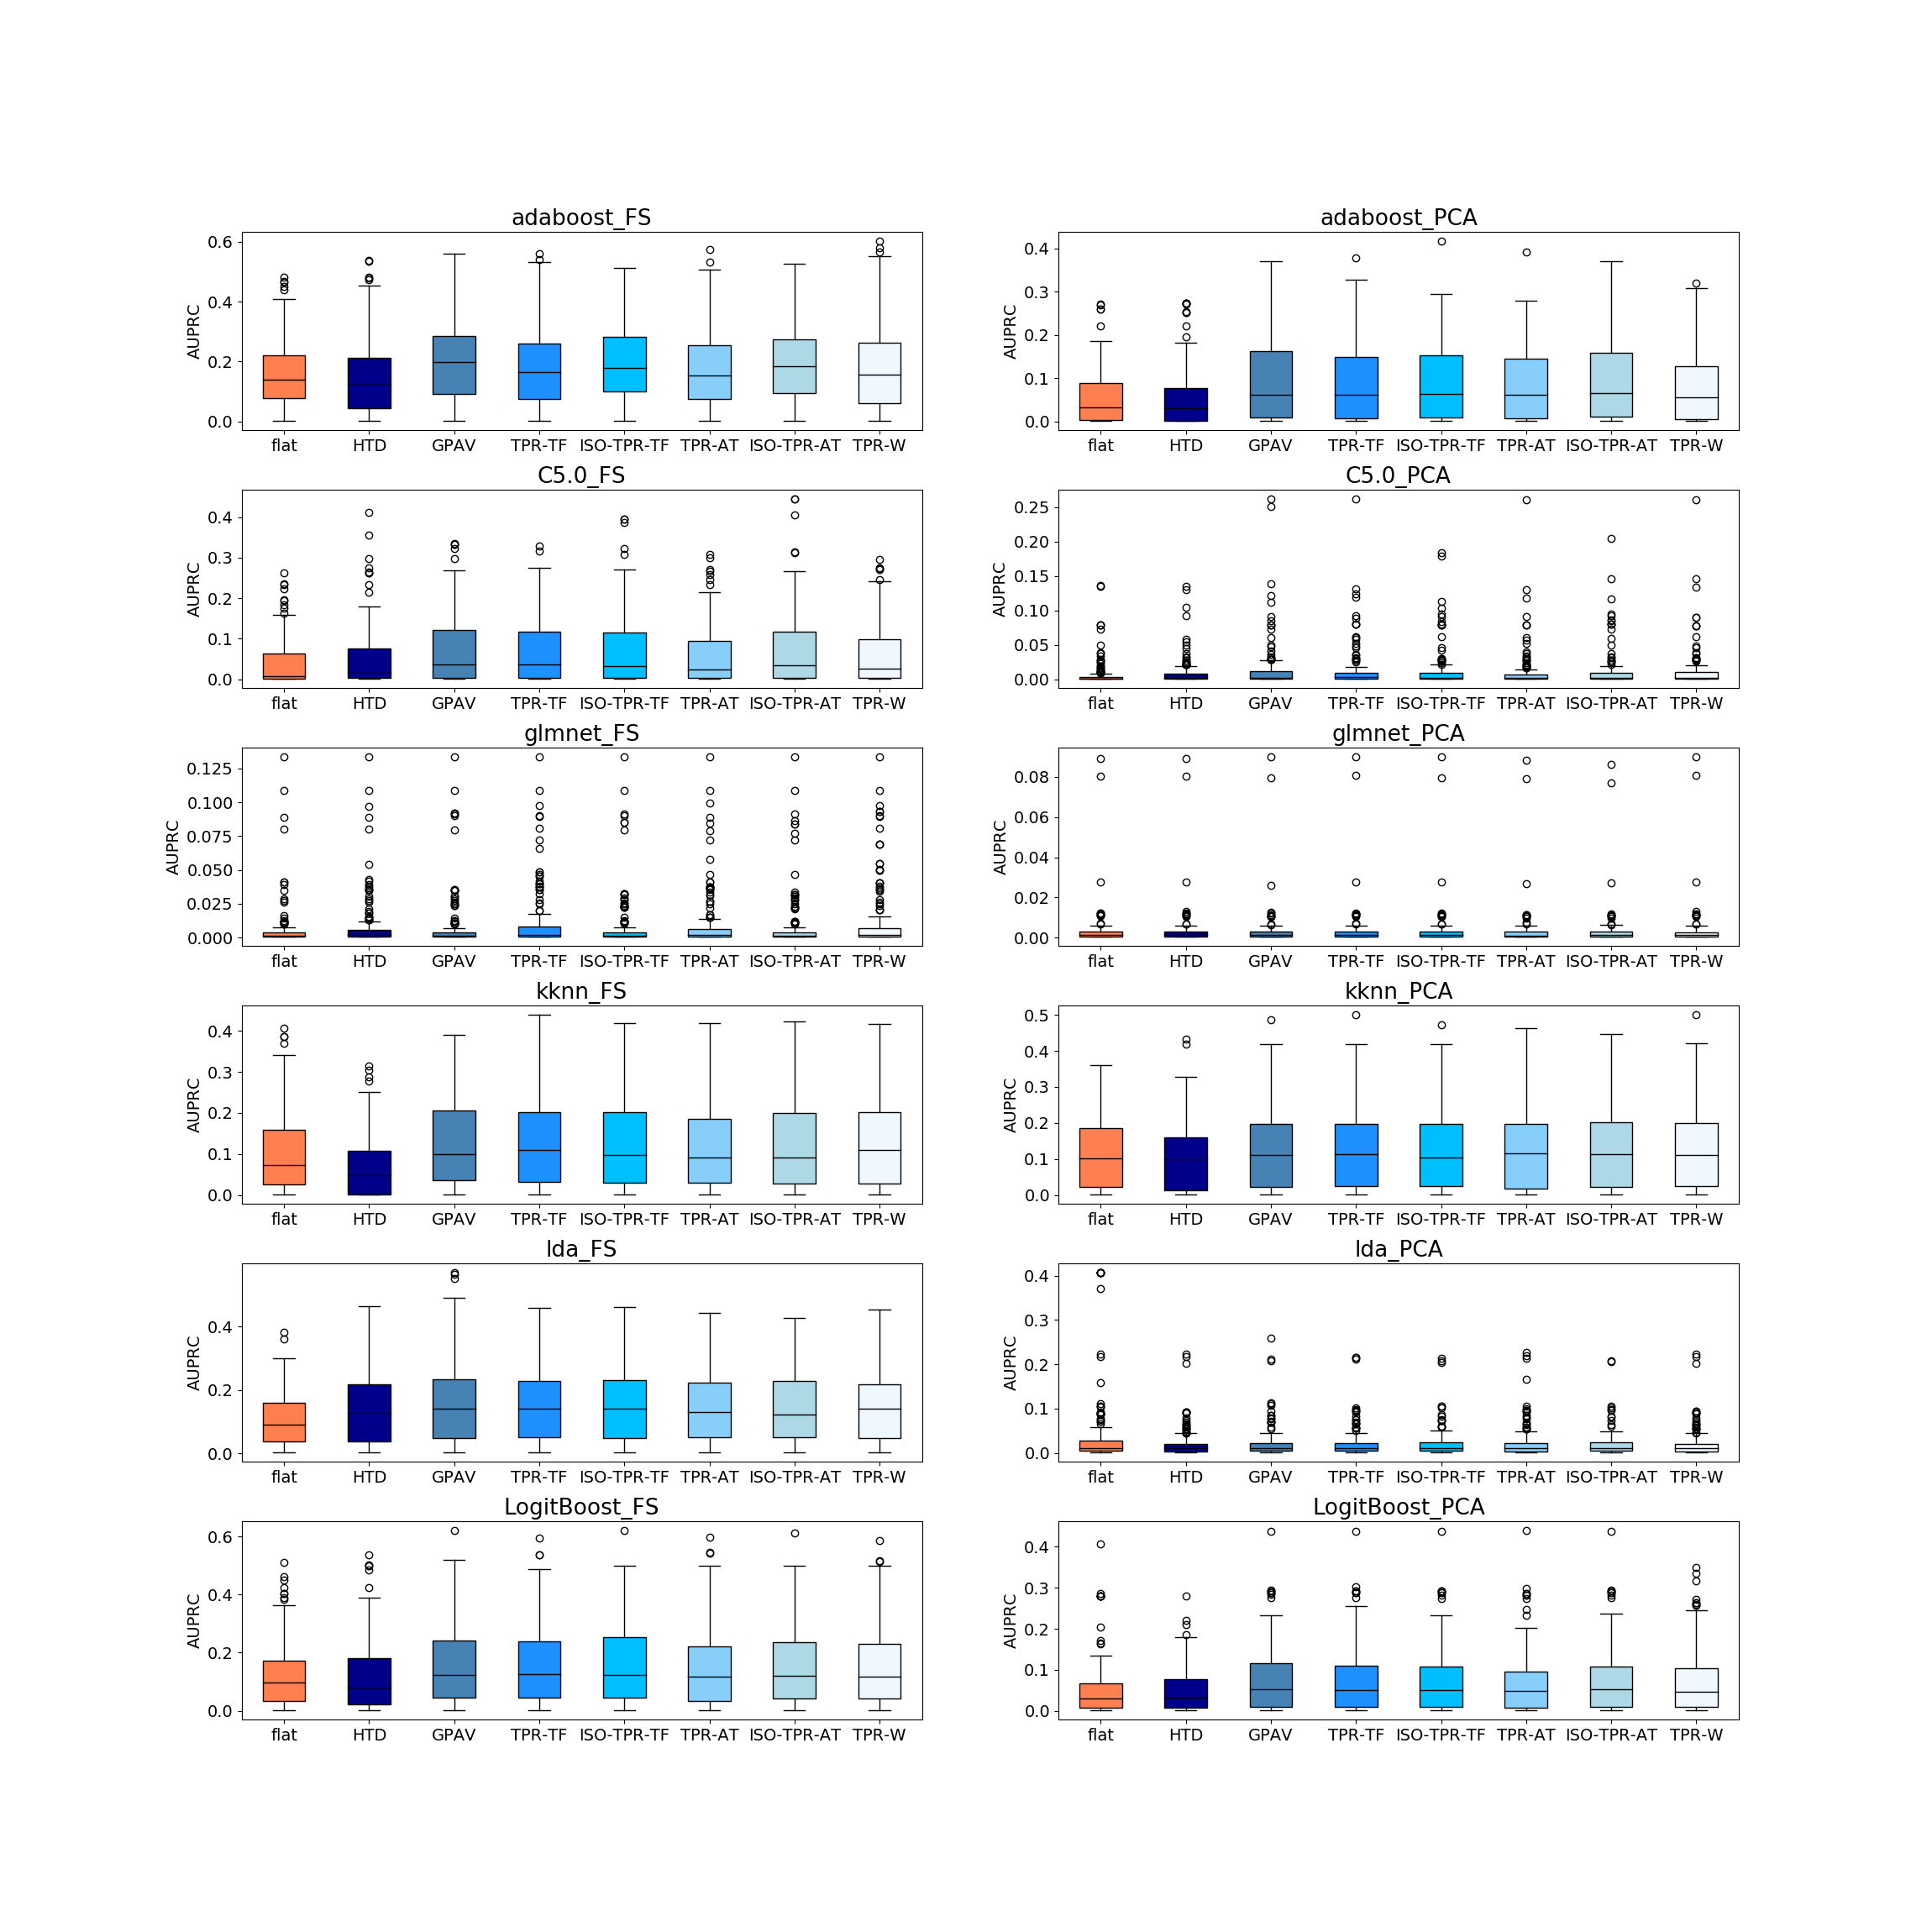
\includegraphics[scale=0.34]{./images/MF_PRC_1.png}
\caption{\footnotesize{Boxplot per l'ontologia MF, relativi alla metrica AUPRC al variare di: metodi gerarchici utilizzati, algoritmi di ML (primi 6) e metodo di riduzione della dimensionalità.}}
\label{MF_PRC_1}
\end{figure}

\begin{figure}[h]
 \hspace*{-2.6cm}
\includegraphics[scale=0.34]{./images/MF_PRC_2.png}
\caption{\footnotesize{Boxplot per l'ontologia MF, relativi alla metrica AUPRC al variare di: metodi gerarchici utilizzati, algoritmi di ML (ultimi 6) e metodo di riduzione della dimensionalità.}}
\label{MF_PRC_2}
\end{figure}

\begin{figure}[h]
 \hspace*{-2.6cm}
\includegraphics[scale=0.34]{./images/CC_PRC_1.png}
\caption{\footnotesize{Boxplot per l'ontologia CC, relativi alla metrica AUPRC al variare di: metodi gerarchici utilizzati, algoritmi di ML (primi 6) e metodo di riduzione della dimensionalità.}}
\label{CC_PRC_1}
\end{figure}


\begin{figure}[h]
 \hspace*{-2.6cm}
\includegraphics[scale=0.34]{./images/CC_PRC_2.png}
\caption{\footnotesize{Boxplot per l'ontologia CC, relativi alla metrica AUPRC al variare di: metodi gerarchici utilizzati, algoritmi di ML (ultimi 6) e metodo di riduzione della dimensionalità.}}
\label{CC_PRC_2}
\end{figure}

\chapter{Tabelle}

\setlength\LTleft{-9mm}
\begin{longtable}[h]{|l|l|l|l|l|l|l|}
\hline
\textbf{Algoritmo}    & \textbf{Onto} & \textbf{feature} & \textbf{AUPRC}  & \textbf{AUROC}  & \textbf{TempoMedio} & \textbf{TempoTotale} \\ \hline
adaboost     & BP   & 1000    & 0,2279 & 0,8429 & 1,44            & 1919,73     \\ \hline
adaboost     & BP   & 500     & 0,1969 & 0,8207 & 0,50            & 666,61      \\ \hline
adaboost     & BP   & 100     & 0,1759 & 0,715  & 0,05            & 64,97       \\ \hline
adaboost     & CC   & 1000    & 0,2002 & 0,8007 & 1,73            & 381,74      \\ \hline
adaboost     & CC   & 500     & 0,2032 & 0,8037 & 0,47            & 102,99      \\ \hline
adaboost     & CC   & 100     & 0,1566 & 0,6931 & 0,05            & 11,49       \\ \hline
adaboost     & MF   & 1000    & 0,2121 & 0,8094 & 1,30            & 242,17      \\ \hline
adaboost     & MF   & 500     & 0,1912 & 0,7661 & 0,47            & 88,04       \\ \hline
adaboost     & MF   & 100     & 0,1227 & 0,6183 & 0,06            & 10,29       \\ \hline
C5.0         & BP   & 1000    & 0,27   & 0,8732 & 0,06            & 78,32       \\ \hline
C5.0         & BP   & 500     & 0,2694 & 0,8686 & 0,03            & 43,61       \\ \hline
C5.0         & BP   & 100     & 0,2336 & 0,7731 & 0,01            & 14,24       \\ \hline
C5.0         & CC   & 1000    & 0,2049 & 0,8612 & 0,09            & 19,30       \\ \hline
C5.0         & CC   & 500     & 0,2137 & 0,8452 & 0,03            & 7,51        \\ \hline
C5.0         & CC   & 100     & 0,2067 & 0,7798 & 0,01            & 2,65        \\ \hline
C5.0         & MF   & 1000    & 0,2686 & 0,8536 & 0,06            & 10,42       \\ \hline
C5.0         & MF   & 500     & 0,2767 & 0,8338 & 0,03            & 5,70        \\ \hline
C5.0         & MF   & 100     & 0,2299 & 0,7299 & 0,01            & 1,98        \\ \hline
glmnet       & BP   & 1000    & 0,0083 & 0,7448 & 0,08            & 104,13      \\ \hline
glmnet       & BP   & 500     & 0,0112 & 0,8176 & 0,05            & 67,64       \\ \hline
glmnet       & BP   & 100     & 0,0288 & 0,8863 & 0,03            & 42,72       \\ \hline
glmnet       & CC   & 1000    & 0,011  & 0,7373 & 0,09            & 20,18       \\ \hline
glmnet       & CC   & 500     & 0,0137 & 0,8113 & 0,05            & 10,02       \\ \hline
glmnet       & CC   & 100     & 0,0311 & 0,9124 & 0,03            & 7,07        \\ \hline
glmnet       & MF   & 1000    & 0,0044 & 0,7148 & 0,06            & 10,42       \\ \hline
glmnet       & MF   & 500     & 0,0067 & 0,7951 & 0,06            & 11,28       \\ \hline
glmnet       & MF   & 100     & 0,0252 & 0,8743 & 0,04            & 7,44        \\ \hline
kknn         & BP   & 1000    & 0,0709 & 0,5618 & 1,01            & 1343,01     \\ \hline
kknn         & BP   & 500     & 0,0828 & 0,5727 & 0,49            & 659,49      \\ \hline
kknn         & BP   & 100     & 0,0874 & 0,564  & 0,14            & 190,46      \\ \hline
kknn         & CC   & 1000    & 0,0694 & 0,5565 & 1,22            & 270,36      \\ \hline
kknn         & CC   & 500     & 0,0727 & 0,5617 & 0,72            & 158,38      \\ \hline
kknn         & CC   & 100     & 0,085  & 0,5666 & 0,06            & 12,97       \\ \hline
kknn         & MF   & 1000    & 0,0217 & 0,5228 & 0,90            & 166,66      \\ \hline
kknn         & MF   & 500     & 0,0265 & 0,5245 & 0,52            & 95,98       \\ \hline
kknn         & MF   & 100     & 0,0289 & 0,5283 & 0,08            & 15,00       \\ \hline
lda          & BP   & 1000    & 0,0137 & 0,5167 & 0,04            & 48,95       \\ \hline
lda          & BP   & 500     & 0,0137 & 0,5167 & 0,02            & 22,25       \\ \hline
lda          & BP   & 100     & 0,0137 & 0,5167 & 0,01            & 8,01        \\ \hline
lda          & CC   & 1000    & 0,006  & 0,5045 & 0,04            & 9,72        \\ \hline
lda          & CC   & 500     & 0,006  & 0,5045 & 0,01            & 3,24        \\ \hline
lda          & CC   & 100     & 0,006  & 0,5045 & 0,01            & 1,47        \\ \hline
lda          & MF   & 1000    & 0,0026 & 0,5005 & 0,04            & 6,57        \\ \hline
lda          & MF   & 500     & 0,0026 & 0,5005 & 0,01            & 2,60        \\ \hline
lda          & MF   & 100     & 0,0026 & 0,5005 & 0,01            & 1,12        \\ \hline
LogitBoost   & BP   & 1000    & 0,1018 & 0,6046 & 0,66            & 882,88      \\ \hline
LogitBoost   & BP   & 500     & 0,1092 & 0,6031 & 0,17            & 229,62      \\ \hline
LogitBoost   & BP   & 100     & 0,1748 & 0,668  & 0,01            & 16,91       \\ \hline
LogitBoost   & CC   & 1000    & 0,1095 & 0,593  & 1,24            & 275,07      \\ \hline
LogitBoost   & CC   & 500     & 0,1142 & 0,6058 & 0,19            & 41,99       \\ \hline
LogitBoost   & CC   & 100     & 0,15   & 0,6633 & 0,01            & 3,09        \\ \hline
LogitBoost   & MF   & 1000    & 0,1875 & 0,6279 & 0,65            & 120,65      \\ \hline
LogitBoost   & MF   & 500     & 0,1954 & 0,6333 & 0,17            & 31,00       \\ \hline
LogitBoost   & MF   & 100     & 0,1683 & 0,6482 & 0,01            & 2,36        \\ \hline
mlp          & BP   & 1000    & 0,1612 & 0,783  & 0,08            & 104,13      \\ \hline
mlp          & BP   & 500     & 0,1729 & 0,812  & 0,04            & 49,84       \\ \hline
mlp          & BP   & 100     & 0,167  & 0,8486 & 0,02            & 20,47       \\ \hline
mlp          & CC   & 1000    & 0,1468 & 0,7221 & 0,08            & 17,68       \\ \hline
mlp          & CC   & 500     & 0,1591 & 0,78   & 0,04            & 9,13        \\ \hline
mlp          & CC   & 100     & 0,1695 & 0,8237 & 0,01            & 2,95        \\ \hline
mlp          & MF   & 1000    & 0,181  & 0,7663 & 0,07            & 13,76       \\ \hline
mlp          & MF   & 500     & 0,1712 & 0,7862 & 0,04            & 7,19        \\ \hline
mlp          & MF   & 100     & 0,1584 & 0,7698 & 0,01            & 2,48        \\ \hline
naive\_bayes & BP   & 1000    & 0,1924 & 0,7537 & 0,01            & 12,46       \\ \hline
naive\_bayes & BP   & 500     & 0,1939 & 0,7467 & 0,01            & 11,57       \\ \hline
naive\_bayes & BP   & 100     & 0,1825 & 0,7393 & 0,01            & 8,01        \\ \hline
naive\_bayes & CC   & 1000    & 0,1705 & 0,7111 & 0,01            & 2,06        \\ \hline
naive\_bayes & CC   & 500     & 0,1634 & 0,7103 & 0,01            & 1,92        \\ \hline
naive\_bayes & CC   & 100     & 0,1893 & 0,7226 & 0,01            & 1,62        \\ \hline
naive\_bayes & MF   & 1000    & 0,1766 & 0,7057 & 0,01            & 1,74        \\ \hline
naive\_bayes & MF   & 500     & 0,1725 & 0,7069 & 0,01            & 1,74        \\ \hline
naive\_bayes & MF   & 100     & 0,1815 & 0,7023 & 0,01            & 1,49        \\ \hline
ranger       & BP   & 1000    & 0,1947 & 0,7029 & 0,02            & 25,81       \\ \hline
ranger       & BP   & 500     & 0,1673 & 0,681  & 0,01            & 18,69       \\ \hline
ranger       & BP   & 100     & 0,1479 & 0,7174 & 0,01            & 13,35       \\ \hline
ranger       & CC   & 1000    & 0,1715 & 0,7141 & 0,02            & 4,71        \\ \hline
ranger       & CC   & 500     & 0,1676 & 0,6938 & 0,02            & 5,45        \\ \hline
ranger       & CC   & 100     & 0,1559 & 0,719  & 0,01            & 1,77        \\ \hline
ranger       & MF   & 1000    & 0,2376 & 0,709  & 0,01            & 2,23        \\ \hline
ranger       & MF   & 500     & 0,2633 & 0,6915 & 0,01            & 2,23        \\ \hline
ranger       & MF   & 100     & 0,1717 & 0,6487 & 0,01            & 1,61        \\ \hline
svmLinear    & BP   & 1000    & 0,292  & 0,8868 & 0,09            & 121,04      \\ \hline
svmLinear    & BP   & 500     & 0,281  & 0,8765 & 0,06            & 85,44       \\ \hline
svmLinear    & BP   & 100     & 0,2623 & 0,8881 & 0,02            & 25,81       \\ \hline
svmLinear    & CC   & 1000    & 0,2277 & 0,8911 & 0,38            & 83,39       \\ \hline
svmLinear    & CC   & 500     & 0,2314 & 0,8961 & 0,17            & 36,83       \\ \hline
svmLinear    & CC   & 100     & 0,2419 & 0,9082 & 0,04            & 8,40        \\ \hline
svmLinear    & MF   & 1000    & 0,2398 & 0,7886 & 0,02            & 4,46        \\ \hline
svmLinear    & MF   & 500     & 0,2428 & 0,8112 & 0,02            & 3,60        \\ \hline
svmLinear    & MF   & 100     & 0,2305 & 0,8192 & 0,05            & 8,43        \\ \hline
treebag      & BP   & 1000    & 0,2688 & 0,9047 & 0,17            & 220,72      \\ \hline
treebag      & BP   & 500     & 0,2951 & 0,8985 & 0,08            & 110,36      \\ \hline
treebag      & BP   & 100     & 0,2794 & 0,8452 & 0,02            & 28,48       \\ \hline
treebag      & CC   & 1000    & 0,2464 & 0,8899 & 0,16            & 35,80       \\ \hline
treebag      & CC   & 500     & 0,2596 & 0,8751 & 0,08            & 17,24       \\ \hline
treebag      & CC   & 100     & 0,2583 & 0,8557 & 0,02            & 4,86        \\ \hline
treebag      & MF   & 1000    & 0,2967 & 0,8607 & 0,13            & 24,43       \\ \hline
treebag      & MF   & 500     & 0,2978 & 0,8483 & 0,07            & 12,52       \\ \hline
treebag      & MF   & 100     & 0,2697 & 0,7833 & 0,02            & 3,84        \\ \hline
xgbLinear    & BP   & 1000    & 0,2575 & 0,9007 & 0,01            & 15,13       \\ \hline
xgbLinear    & BP   & 500     & 0,2661 & 0,8911 & 0,01            & 13,35       \\ \hline
xgbLinear    & BP   & 100     & 0,2664 & 0,8489 & 0,01            & 10,68       \\ \hline
xgbLinear    & CC   & 1000    & 0,2407 & 0,8998 & 0,05            & 11,49       \\ \hline
xgbLinear    & CC   & 500     & 0,2378 & 0,8879 & 0,01            & 2,36        \\ \hline
xgbLinear    & CC   & 100     & 0,2502 & 0,8685 & 0,01            & 2,21        \\ \hline
xgbLinear    & MF   & 1000    & 0,282  & 0,8549 & 0,01            & 1,36        \\ \hline
xgbLinear    & MF   & 500     & 0,2742 & 0,8507 & 0,01            & 1,12        \\ \hline
xgbLinear    & MF   & 100     & 0,2671 & 0,8045 & 0,01            & 1,61        \\ \hline
\caption{Le stime per classe (ad eccezione di Tempo Totale, che considera tutte le classi) ottenute dalla selezione delle feature a 5 fold con 3 differenti configurazioni per le feature (100, 500, 1000) su un campione di 10 classi per ontologia. I tempi sono espressi in ore.}
\label{featureSelection}
\end{longtable}

\begin{longtable}[h]{|l|l|l|l|l|l|l|l|}
\hline
\textbf{Algoritmo} & \textbf{Onto} & \textbf{Var} & \textbf{\#comp} & \textbf{AUPRC} & \textbf{AUROC} & \textbf{TempoMed} & \textbf{TempoTot} \\ \hline
adaboost           & BP            & 90                & 1000               & 0,1442         & 0,8245         & 3,642                    & 4862,07              \\ \hline
adaboost           & BP            & 70                & 100                & 0,1695         & 0,8016         & 0,485                    & 647,475              \\ \hline
adaboost           & BP            & 50                & 15                 & 0,0857         & 0,7363         & 0,212                    & 283,02               \\ \hline
adaboost           & CC            & 90                & 1000               & 0,1887         & 0,808          & 4,348                    & 960,908              \\ \hline
adaboost           & CC            & 70                & 100                & 0,2059         & 0,7873         & 0,759                    & 167,739              \\ \hline
adaboost           & CC            & 50                & 15                 & 0,1152         & 0,7227         & 0,306                    & 67,626               \\ \hline
adaboost           & MF            & 90                & 1000               & 0,1859         & 0,7783         & 2,999                    & 557,814              \\ \hline
adaboost           & MF            & 70                & 100                & 0,1962         & 0,7844         & 0,763                    & 141,918              \\ \hline
adaboost           & MF            & 50                & 15                 & 0,1533         & 0,7213         & 0,133                    & 24,738               \\ \hline
C5.0               & BP            & 90                & 1000               & 0,0378         & 0,545          & 0,398                    & 531,33               \\ \hline
C5.0               & BP            & 70                & 100                & 0,0367         & 0,5328         & 0,034                    & 45,39                \\ \hline
C5.0               & BP            & 50                & 15                 & 0,0062         & 0,5098         & 0,007                    & 9,345                \\ \hline
C5.0               & CC            & 90                & 1000               & 0,0578         & 0,5672         & 0,53                     & 117,13               \\ \hline
C5.0               & CC            & 70                & 100                & 0,0625         & 0,571          & 0,044                    & 9,724                \\ \hline
C5.0               & CC            & 50                & 15                 & 0,0305         & 0,5356         & 0,01                     & 2,21                 \\ \hline
C5.0               & MF            & 90                & 1000               & 0,0325         & 0,5365         & 0,608                    & 113,088              \\ \hline
C5.0               & MF            & 70                & 100                & 0,0472         & 0,5469         & 0,024                    & 4,464                \\ \hline
C5.0               & MF            & 50                & 15                 & 0,0088         & 0,5202         & 0,006                    & 1,116                \\ \hline
glmnet             & BP            & 90                & 1000               & 0,0049         & 0,5            & 0,145                    & 193,575              \\ \hline
glmnet             & BP            & 70                & 100                & 0,0049         & 0,5            & 0,126                    & 168,21               \\ \hline
glmnet             & BP            & 50                & 15                 & 0,0049         & 0,5            & 0,005                    & 6,675                \\ \hline
glmnet             & CC            & 90                & 1000               & 0,0132         & 0,5            & 0,461                    & 101,881              \\ \hline
glmnet             & CC            & 70                & 100                & 0,0132         & 0,5            & 0,424                    & 93,704               \\ \hline
glmnet             & CC            & 50                & 15                 & 0,0132         & 0,5            & 0,01                     & 2,21                 \\ \hline
glmnet             & MF            & 90                & 1000               & 0,0026         & 0,5            & 0,159                    & 29,574               \\ \hline
glmnet             & MF            & 70                & 100                & 0,0026         & 0,5            & 0,459                    & 85,374               \\ \hline
glmnet             & MF            & 50                & 15                 & 0,0026         & 0,5            & 0,014                    & 2,604                \\ \hline
knn                & BP            & 90                & 1000               & 0,1701         & 0,6747         & 0,573                    & 764,955              \\ \hline
knn                & BP            & 70                & 100                & 0,1443         & 0,6831         & 0,049                    & 65,415               \\ \hline
knn                & BP            & 50                & 15                 & 0,076          & 0,6482         & 0,004                    & 5,34                 \\ \hline
knn                & CC            & 90                & 1000               & 0,1608         & 0,6947         & 0,714                    & 157,794              \\ \hline
knn                & CC            & 70                & 100                & 0,1314         & 0,6656         & 0,061                    & 13,481               \\ \hline
knn                & CC            & 50                & 15                 & 0,0835         & 0,6307         & 0,007                    & 1,547                \\ \hline
knn                & MF            & 90                & 1000               & 0,1929         & 0,7106         & 0,858                    & 159,588              \\ \hline
knn                & MF            & 70                & 100                & 0,1874         & 0,7182         & 0,039                    & 7,254                \\ \hline
knn                & MF            & 50                & 15                 & 0,1292         & 0,6952         & 0,003                    & 0,558                \\  \hline
lda                & BP            & 90                & 1000               & 0,1988         & 0,8459         & 0,113                    & 150,855              \\ \hline
lda                & BP            & 70                & 100                & 0,1381         & 0,8859         & 0,004                    & 5,34                 \\ \hline
lda                & BP            & 50                & 15                 & 0,0337         & 0,8168         & 0,002                    & 2,67                 \\ \hline
lda                & CC            & 90                & 1000               & 0,2697         & 0,8493         & 0,167                    & 36,907               \\ \hline
lda                & CC            & 70                & 100                & 0,1803         & 0,8725         & 0,007                    & 1,547                \\ \hline
lda                & CC            & 50                & 15                 & 0,0638         & 0,8064         & 0,003                    & 0,663                \\ \hline
lda                & MF            & 90                & 1000               & 0,2238         & 0,883          & 0,099                    & 18,414               \\ \hline
lda                & MF            & 70                & 100                & 0,1245         & 0,8594         & 0,003                    & 0,558                \\ \hline
lda                & MF            & 50                & 15                 & 0,0706         & 0,8061         & 0,001                    & 0,186                \\ \hline
mlp                & BP            & 90                & 1000               & 0,0607         & 0,7629         & 0,183                    & 244,305              \\ \hline
mlp                & BP            & 70                & 100                & 0,0626         & 0,7026         & 0,026                    & 34,71                \\ \hline
mlp                & BP            & 50                & 15                 & 0,0208         & 0,666          & 0,017                    & 22,695               \\ \hline
mlp                & CC            & 90                & 1000               & 0,1301         & 0,7017         & 0,246                    & 54,366               \\ \hline
mlp                & CC            & 70                & 100                & 0,1045         & 0,6157         & 0,032                    & 7,072                \\ \hline
mlp                & CC            & 50                & 15                 & 0,049          & 0,6289         & 0,02                     & 4,42                 \\ \hline
mlp                & MF            & 90                & 1000               & 0,027          & 0,7138         & 0,354                    & 65,844               \\ \hline
mlp                & MF            & 70                & 100                & 0,0154         & 0,6251         & 0,024                    & 4,464                \\ \hline
mlp                & MF            & 50                & 15                 & 0,0139         & 0,6594         & 0,014                    & 2,604                \\ \hline
svmLinear          & BP            & 90                & 1000               & 0,2228         & 0,8118         & 0,106                    & 141,51               \\ \hline
svmLinear          & BP            & 70                & 100                & 0,1333         & 0,7555         & 0,017                    & 22,695               \\ \hline
svmLinear          & BP            & 50                & 15                 & 0,0136         & 0,5497         & 0,007                    & 9,345                \\ \hline
svmLinear          & CC            & 90                & 1000               & 0,262          & 0,8075         & 0,23                     & 50,83                \\ \hline
svmLinear          & CC            & 70                & 100                & 0,1595         & 0,6955         & 0,027                    & 5,967                \\ \hline
svmLinear          & CC            & 50                & 15                 & 0,0229         & 0,5534         & 0,011                    & 2,431                \\ \hline
svmLinear          & MF            & 90                & 1000               & 0,2567         & 0,8545         & 0,162                    & 30,132               \\ \hline
svmLinear          & MF            & 70                & 100                & 0,1286         & 0,7354         & 0,011                    & 2,046                \\ \hline
svmLinear          & MF            & 50                & 15                 & 0,0329         & 0,6031         & 0,005                    & 0,93                 \\ \hline
treebag            & BP            & 90                & 1000               & 0,0894         & 0,664          & 1,281                    & 1710,135             \\ \hline
treebag            & BP            & 70                & 100                & 0,1033         & 0,6849         & 0,12                     & 160,2                \\ \hline
treebag            & BP            & 50                & 15                 & 0,0572         & 0,6412         & 0,015                    & 20,025               \\ \hline
treebag            & CC            & 90                & 1000               & 0,1175         & 0,664          & 2,032                    & 449,072              \\ \hline
treebag            & CC            & 70                & 100                & 0,1577         & 0,6879         & 0,173                    & 38,233               \\ \hline
treebag            & CC            & 50                & 15                 & 0,089          & 0,6378         & 0,022                    & 4,862                \\ \hline
treebag            & MF            & 90                & 1000               & 0,1426         & 0,6601         & 1,041                    & 193,626              \\ \hline
treebag            & MF            & 70                & 100                & 0,1655         & 0,6715         & 0,093                    & 17,298               \\ \hline
treebag            & MF            & 50                & 15                 & 0,1071         & 0,6448         & 0,011                    & 2,046                \\ \hline
xgbLinear          & BP            & 90                & 1000               & 0,1855         & 0,832          & 0,048                    & 64,08                \\ \hline
xgbLinear          & BP            & 70                & 100                & 0,1866         & 0,821          & 0,02                     & 26,7                 \\ \hline
xgbLinear          & BP            & 50                & 15                 & 0,0991         & 0,7935         & 0,015                    & 20,025               \\ \hline
xgbLinear          & CC            & 90                & 1000               & 0,2078         & 0,8172         & 0,065                    & 14,365               \\ \hline
xgbLinear          & CC            & 70                & 100                & 0,2073         & 0,7934         & 0,029                    & 6,409                \\ \hline
xgbLinear          & CC            & 50                & 15                 & 0,1168         & 0,75           & 0,021                    & 4,641                \\ \hline
xgbLinear          & MF            & 90                & 1000               & 0,1982         & 0,8123         & 0,04                     & 7,44                 \\ \hline
xgbLinear          & MF            & 70                & 100                & 0,1987         & 0,7825         & 0,009                    & 1,674                \\ \hline
xgbLinear          & MF            & 50                & 15                 & 0,1297         & 0,7722         & 0,009                    & 1,674                \\ \hline
\caption{\footnotesize{Le stime per classe (ad eccezione di Tempo Totale, che considera tutte le classi) ottenute con cross-validation a 10 fold, con diversi livelli di selezione della varianza (90\%, 70\% e 50\%) su un campione di 10 classi per ontologia. I tempi sono espressi in ore.}}
\label{diffvariance}
\end{longtable}

\begin{table}[h]
\centering
\begin{tabular}{|l|l|l|l|l|l|}
\hline
\textbf{Algoritmo} & \textbf{Onto} & \textbf{AUPRC} & \textbf{AUROC} & \textbf{TempoMedio} & \textbf{TempoTotale} \\ \hline
adaboost           & BP            & 0,0447         & 0,5861         & 0,0028                   & 3,6718               \\ \hline
adaboost           & CC            & 0,066          & 0,6071         & 0,0028                   & 0,6093               \\ \hline
adaboost           & MF            & 0,0707         & 0,6205         & 0,0027                   & 0,4996               \\ \hline
C5.0               & BP            & 0,0017         & 0,5            & 0,0029                   & 3,9018               \\ \hline
C5.0               & CC            & 0,0257         & 0,5419         & 0,0026                   & 0,5707               \\ \hline
C5.0               & MF            & 0,0128         & 0,5161         & 0,0031                   & 0,5705               \\ \hline
glmnet             & BP            & 0,0017         & 0,5            & 0,0025                   & 3,3391               \\ \hline
glmnet             & CC            & 0,0059         & 0,5            & 0,0031                   & 0,6764               \\ \hline
glmnet             & MF            & 0,0026         & 0,5            & 0,005                    & 0,9216               \\ \hline
kknn               & BP            & 0,0554         & 0,5949         & 0,0109                   & 14,49                \\ \hline
kknn               & CC            & 0,0973         & 0,6333         & 0,0093                   & 2,0456               \\ \hline
kknn               & MF            & 0,1305         & 0,6555         & 0,0098                   & 1,8138               \\ \hline
lda                & BP            & 0,0317         & 0,8018         & 0,0007                   & 0,9604               \\ \hline
lda                & CC            & 0,0513         & 0,8743         & 0,0008                   & 0,1819               \\ \hline
lda                & MF            & 0,0528         & 0,8124         & 0,0009                   & 0,1756               \\ \hline
LogitBoost         & BP            & 0,0147         & 0,7486         & 0,001                    & 1,2772               \\ \hline
LogitBoost         & CC            & 0,0441         & 0,8127         & 0,001                    & 0,2107               \\ \hline
LogitBoost         & MF            & 0,0677         & 0,7781         & 0,001                    & 0,178                \\ \hline
mlp                & BP            & 0,0045         & 0,5683         & 0,0061                   & 8,1541               \\ \hline
mlp                & CC            & 0,0298         & 0,5963         & 0,0056                   & 1,2439               \\ \hline
mlp                & MF            & 0,0099         & 0,6305         & 0,0056                   & 1,0506               \\ \hline
naive\_bayes       & BP            & 0,011          & 0,7224         & 0,0007                   & 0,9106               \\ \hline
naive\_bayes       & CC            & 0,0259         & 0,7417         & 0,0007                   & 0,1505               \\ \hline
naive\_bayes       & MF            & 0,0243         & 0,7163         & 0,0007                   & 0,1271               \\ \hline
ranger             & BP            & 0,052          & 0,7826         & 0,0021                   & 2,7632               \\ \hline
ranger             & CC            & 0,1288         & 0,8092         & 0,0024                   & 0,522                \\ \hline
ranger             & MF            & 0,1522         & 0,8124         & 0,0021                   & 0,3854               \\ \hline
svmLinear2         & BP            & 0,0058         & 0,537          & 0,0027                   & 3,6499               \\ \hline
svmLinear2         & CC            & 0,01           & 0,5413         & 0,0042                   & 0,9206               \\ \hline
svmLinear2         & MF            & 0,0113         & 0,5697         & 0,0032                   & 0,6006               \\ \hline
treebag            & BP            & 0,0246         & 0,5897         & 0,0042                   & 5,5443               \\ \hline
treebag            & CC            & 0,0773         & 0,6521         & 0,0044                   & 0,974                \\ \hline
treebag            & MF            & 0,086          & 0,6488         & 0,0043                   & 0,7982               \\ \hline
xgbLinear          & BP            & 0,0365         & 0,7677         & 0,0029                   & 3,89                 \\ \hline
xgbLinear          & CC            & 0,0966         & 0,7919         & 0,0034                   & 0,7607               \\ \hline
xgbLinear          & MF            & 0,0976         & 0,7863         & 0,0029                   & 0,5453               \\ \hline
\end{tabular}
\caption{Le stime per classe (ad eccezione di Tempo Totale, che considera tutte le classi) per PCA con selezione di 15 componenti (50\% di varianza spiegata) e cross-validation 5 fold , su un campione di 10 classi per ontologia. I tempi sono espressi in ore.}
\label{PCA5fold}
\end{table}

\begin{table}[h!]
\centering
\small\caption*{\textbf{Confronto fra metodi gerarchici e metodi flat specifici con FS (AUROC).}}
\resizebox{1\textwidth}{!}{
\begin{tabular}{|l|l|l|l|l|l|l|l|l|}
\hline
\textbf{AUROC}         & \textbf{GPAV} & \textbf{HTD} & \textbf{TPR-TF} & \textbf{ISO-TPR-TF} & \textbf{TPR-AT} & \textbf{ISO-TPR-AT} & \textbf{TPR-W} & \textbf{SommeXrighe} \\ \hline
\textbf{adaboost}      & 3             & 0            & 3               & 3                   & 1               & 3                   & 3              & 16/21                \\ \hline
\textbf{C5.0}          & 3             & 2            & 3               & 3                   & 3               & 3                   & 3              & 20/21                \\ \hline
\textbf{glmnet}        & 1             & 0            & 0               & 1                   & 0               & 0                   & 0              & 2/21                 \\ \hline
\textbf{kknn}          & 3             & 0            & 3               & 3                   & 2               & 3                   & 3              & 17/21                \\ \hline
\textbf{lda}           & 3             & 0            & 3               & 3                   & 3               & 3                   & 3              & 18/21                \\ \hline
\textbf{LogitBoost}    & 3             & 0            & 3               & 3                   & 0               & 3                   & 3              & 15/21                \\ \hline
\textbf{mlp}           & 3             & 0            & 3               & 3                   & 0               & 3                   & 2              & 14/21                \\ \hline
\textbf{naive\_bayes}  & 3             & 0            & 3               & 3                   & 3               & 3                   & 3              & 18/21                \\ \hline
\textbf{ranger}        & 3             & 0            & 3               & 3                   & 0               & 3                   & 3              & 15/21                \\ \hline
\textbf{svmLinear2}    & 3             & 0            & 3               & 3                   & 0               & 3                   & 2              & 14/21                \\ \hline
\textbf{treebag}       & 3             & 0            & 3               & 3                   & 0               & 3                   & 3              & 15/21                \\ \hline
\textbf{xgbLinear}     & 3             & 0            & 3               & 3                   & 3               & 3                   & 3              & 18/21                \\ \hline
\textbf{SommeXcolonne} & 34/36         & 2/34         & 33/36           & 34/36               & 15/36           & 33/36               & 31/36          &                      \\ \hline
\end{tabular}}

\centering
\small\caption*{\textbf{Confronto fra metodi gerarchici e metodi flat specifici con PCA (AUROC).}}
\resizebox{1\textwidth}{!}{
\begin{tabular}{|l|l|l|l|l|l|l|l|l|}
\hline
\textbf{AUROC}         & \textbf{GPAV} & \textbf{HTD} & \textbf{TPR-TF} & \textbf{ISO-TPR-TF} & \textbf{TPR-AT} & \textbf{ISO-TPR-AT} & \textbf{TPR-W} & \textbf{SommeXrighe} \\ \hline
\textbf{adaboost}      & 3             & 0            & 3               & 3                   & 2               & 3                   & 3              & 17/21                \\ \hline
\textbf{C5.0}          & 2             & 3            & 3               & 1                   & 3               & 1                   & 3              & 16/21                \\ \hline
\textbf{glmnet}        & 0             & 0            & 0               & 0                   & 0               & 0                   & 0              & 0/21                 \\ \hline
\textbf{kknn}          & 3             & 0            & 3               & 3                   & 0               & 3                   & 3              & 15/21                \\ \hline
\textbf{lda}           & 0             & 1            & 1               & 0                   & 1               & 0                   & 2              & 5/21                 \\ \hline
\textbf{LogitBoost}    & 3             & 3            & 3               & 3                   & 3               & 3                   & 3              & 21/21                \\ \hline
\textbf{mlp}           & 3             & 3            & 3               & 0                   & 3               & 1                   & 3              & 16/21                \\ \hline
\textbf{naive\_bayes}  & 0             & 2            & 0               & 0                   & 1               & 0                   & 0              & 3/21                 \\ \hline
\textbf{ranger}        & 3             & 0            & 3               & 3                   & 0               & 3                   & 3              & 15/21                \\ \hline
\textbf{svmLinear2}    & 0             & 3            & 0               & 0                   & 1               & 0                   & 1              & 5/21                 \\ \hline
\textbf{treebag}       & 3             & 0            & 3               & 3                   & 0               & 3                   & 3              & 15/21                \\ \hline
\textbf{xgbLinear}     & 3             & 3            & 3               & 3                   & 3               & 3                   & 3              & 21/21                \\ \hline
\textbf{SommeXcolonne} & 23/36         & 18/36        & 25/36           & 19/36               & 17/36           & 20/36               & 27/36          &                      \\ \hline
\end{tabular}}
\caption{\footnotesize{Confronto delle performance (AUROC) metodi flat - metodi gerarchici per ogni metodo flat utilizzato. Ogni entry delle tabelle conta per quante ontologie (BP, MF, CC) esiste una differenza significativa fra il metodo gerarchico ed il metodo flat, e il valore atteso della metrica risulta superiore per il metodo ensemble (Wilcoxon rank sum test, $\alpha = 0.01$).}}
\label{AUROC_1_}
\end{table}

\begin{table}[h!]
\centering
\small\caption*{\textbf{Confronto fra metodi gerarchici e metodi flat specifici con FS (AUPRC).}}
\resizebox{1\textwidth}{!}{
\begin{tabular}{|l|l|l|l|l|l|l|l|l|}
\hline
\textbf{AUPRC}         & \textbf{GPAV} & \textbf{HTD} & \textbf{TPR-TF} & \textbf{ISO-TPR-TF} & \textbf{TPR-AT} & \textbf{ISO-TPR-AT} & \textbf{TPR-W} & \textbf{SommeXrighe} \\ \hline
\textbf{adaboost}      & 3             & 0            & 3               & 3                   & 3               & 3                   & 3              & 18/21                \\ \hline
\textbf{C5.0}          & 3             & 0            & 3               & 3                   & 3               & 3                   & 3              & 18/21                \\ \hline
\textbf{glmnet}        & 1             & 2            & 1               & 1                   & 1               & 1                   & 1              & 8/21                 \\ \hline
\textbf{kknn}          & 3             & 0            & 3               & 3                   & 3               & 3                   & 3              & 18/21                \\ \hline
\textbf{lda}           & 3             & 3            & 3               & 3                   & 3               & 3                   & 3              & 21/21                \\ \hline
\textbf{LogitBoost}    & 3             & 0            & 3               & 3                   & 3               & 3                   & 3              & 18/21                \\ \hline
\textbf{mlp}           & 3             & 0            & 2               & 3                   & 0               & 3                   & 0              & 11/21                \\ \hline
\textbf{naive\_bayes}  & 3             & 3            & 3               & 3                   & 3               & 3                   & 3              & 21/21                \\ \hline
\textbf{ranger}        & 3             & 0            & 3               & 3                   & 1               & 3                   & 3              & 16/21                \\ \hline
\textbf{svmLinear2}    & 3             & 0            & 3               & 3                   & 3               & 3                   & 3              & 18/21                \\ \hline
\textbf{treebag}       & 3             & 0            & 3               & 3                   & 3               & 3                   & 3              & 18/21                \\ \hline
\textbf{xgbLinear}     & 3             & 0            & 3               & 3                   & 2               & 3                   & 3              & 17/21                \\ \hline
\textbf{SommeXcolonne} & 34/36         & 8/36         & 33/36           & 34/36               & 28/36           & 34/36               & 31/36          &                      \\ \hline
\end{tabular}}


\centering
\small\caption*{\textbf{Confronto fra metodi gerarchici e metodi flat specifici con PCA (AUPRC).}}
\resizebox{1\textwidth}{!}{
\begin{tabular}{|l|l|l|l|l|l|l|l|l|}
\hline
\textbf{AUPRC}                  & \textbf{GPAV} & \textbf{HTD} & \textbf{TPR-TF} & \textbf{ISO-TPR-TF} & \textbf{TPR-AT} & \textbf{ISO-TPR-AT} & \textbf{TPR-W} & \textbf{SommeXrighe} \\ \hline
\textbf{adaboost}      & 3             & 0            & 3               & 3                   & 3               & 3                   & 3              & 18/21                \\ \hline
\textbf{C5.0}          & 3             & 3            & 3               & 2                   & 3               & 1                   & 2              & 17/21                \\ \hline
\textbf{glmnet}        & 0             & 0            & 1               & 0                   & 0               & 0                   & 1              & 2/21                 \\ \hline
\textbf{kknn}          & 3             & 0            & 3               & 3                   & 1               & 2                   & 3              & 15/21                \\ \hline
\textbf{lda}           & 1             & 1            & 1               & 0                   & 0               & 0                   & 1              & 4/21                 \\ \hline
\textbf{LogitBoost}    & 3             & 0            & 3               & 3                   & 3               & 3                   & 3              & 18/21                \\ \hline
\textbf{mlp}           & 0             & 3            & 2               & 0                   & 2               & 0                   & 2              & 9/21                 \\ \hline
\textbf{naive\_bayes}  & 0             & 2            & 0               & 0                   & 1               & 0                   & 0              & 3/21                 \\ \hline
\textbf{ranger}        & 3             & 0            & 3               & 3                   & 2               & 3                   & 3              & 17/21                \\ \hline
\textbf{svmLinear2}    & 0             & 1            & 0               & 0                   & 0               & 0                   & 0              & 1/21                 \\ \hline
\textbf{treebag}       & 3             & 3            & 3               & 3                   & 3               & 3                   & 3              & 21/21                \\ \hline
\textbf{xgbLinear}     & 3             & 2            & 3               & 3                   & 3               & 3                   & 3              & 20/21                \\ \hline
\textbf{SommeXcolonne} & 22/36         & 15/36        & 25/36           & 20/36               & 21/36           & 18/36               & 24/36          &                      \\ \hline
\end{tabular}}
\caption{\footnotesize{Confronto delle performance (AUPRC) metodi flat - metodi gerarchici per ogni metodo flat utilizzato. Ogni entry delle tabelle conta per quante ontologie (BP, MF, CC) esiste una differenza significativa fra il metodo gerarchico ed il metodo flat, e il valore atteso della metrica risulta superiore per il metodo ensemble (Wilcoxon rank sum test, $\alpha = 0.01$).}}
\label{AUPRC_1_}
\end{table}



\begin{table}[h!]

\hspace*{-0.45in}
                    \resizebox{.4\textwidth}{!}{
                    \begin{subtable}[t]{0.4\textwidth}
                    \centering\footnotesize
\caption{ \textbf{[AUROC] [BP] [FS]}}
\begin{tabular}{|l|l|l|l|l|l|l|l|}
\hline
 \textbf{WIN / LOSE} & \textbf{GPAV} & \textbf{HTD} & \textbf{TPR-TF} & \textbf{ISO-TPR-TF} & \textbf{TPR-AT} & \textbf{ISO-TPR-AT} & \textbf{TPR-W} \\ \hline
 \textbf{GPAV} & 0/0 & 11/12 & 9/12 & 6/12 & 12/12 & 8/12 & 8/12 \\ \hline
 \textbf{HTD} & 0/12 & 0/0 & 1/12 & 0/12 & 1/12 & 0/12 & 0/12 \\ \hline
 \textbf{TPR-TF} & 0/12 & 11/12 & 0/0 & 3/12 & 12/12 & 1/12 & 7/12 \\ \hline
 \textbf{ISO-TPR-TF} & 3/12 & 11/12 & 8/12 & 0/0 & 11/12 & 5/12 & 9/12 \\ \hline
 \textbf{TPR-AT} & 0/12 & 11/12 & 0/12 & 0/12 & 0/0 & 0/12 & 0/12 \\ \hline
 \textbf{ISO-TPR-AT} & 2/12 & 11/12 & 6/12 & 4/12 & 11/12 & 0/0 & 6/12 \\ \hline
 \textbf{TPR-W} & 2/12 & 11/12 & 3/12 & 1/12 & 12/12 & 2/12 & 0/0 \\ \hline
\end{tabular}

                    \label{table1}
                    \end{subtable}}\par\bigskip

\hspace*{-0.45in}
                    \resizebox{.4\textwidth}{!}{
                    \begin{subtable}[t]{0.4\textwidth}
                    \centering\footnotesize
\caption{ \textbf{[AUROC] [MF] [FS]}}
\begin{tabular}{|l|l|l|l|l|l|l|l|}
\hline
 \textbf{WIN / LOSE} & \textbf{GPAV} & \textbf{HTD} & \textbf{TPR-TF} & \textbf{ISO-TPR-TF} & \textbf{TPR-AT} & \textbf{ISO-TPR-AT} & \textbf{TPR-W} \\ \hline
 \textbf{GPAV} & 0/0 & 11/12 & 3/12 & 6/12 & 11/12 & 9/12 & 3/12 \\ \hline
 \textbf{HTD} & 1/12 & 0/0 & 1/12 & 1/12 & 1/12 & 1/12 & 1/12 \\ \hline
 \textbf{TPR-TF} & 0/12 & 11/12 & 0/0 & 3/12 & 11/12 & 3/12 & 4/12 \\ \hline
 \textbf{ISO-TPR-TF} & 2/12 & 11/12 & 3/12 & 0/0 & 10/12 & 4/12 & 4/12 \\ \hline
 \textbf{TPR-AT} & 0/12 & 11/12 & 0/12 & 0/12 & 0/0 & 0/12 & 0/12 \\ \hline
 \textbf{ISO-TPR-AT} & 0/12 & 10/12 & 1/12 & 3/12 & 10/12 & 0/0 & 2/12 \\ \hline
 \textbf{TPR-W} & 1/12 & 11/12 & 0/12 & 2/12 & 11/12 & 3/12 & 0/0 \\ \hline
\end{tabular}

                    \label{table1}
                    \end{subtable}}\par\bigskip

\hspace*{-0.45in}
                    \resizebox{.4\textwidth}{!}{
                    \begin{subtable}[t]{0.4\textwidth}
                    \centering\footnotesize
\caption{ \textbf{[AUROC] [CC] [FS]}}
\begin{tabular}{|l|l|l|l|l|l|l|l|}
\hline
 \textbf{WIN / LOSE} & \textbf{GPAV} & \textbf{HTD} & \textbf{TPR-TF} & \textbf{ISO-TPR-TF} & \textbf{TPR-AT} & \textbf{ISO-TPR-AT} & \textbf{TPR-W} \\ \hline
 \textbf{GPAV} & 0/0 & 11/12 & 8/12 & 4/12 & 11/12 & 7/12 & 9/12 \\ \hline
 \textbf{HTD} & 0/12 & 0/0 & 0/12 & 0/12 & 0/12 & 1/12 & 0/12 \\ \hline
 \textbf{TPR-TF} & 0/12 & 11/12 & 0/0 & 1/12 & 11/12 & 0/12 & 7/12 \\ \hline
 \textbf{ISO-TPR-TF} & 3/12 & 11/12 & 6/12 & 0/0 & 11/12 & 6/12 & 8/12 \\ \hline
 \textbf{TPR-AT} & 0/12 & 11/12 & 0/12 & 0/12 & 0/0 & 0/12 & 0/12 \\ \hline
 \textbf{ISO-TPR-AT} & 1/12 & 11/12 & 4/12 & 1/12 & 11/12 & 0/0 & 9/12 \\ \hline
 \textbf{TPR-W} & 2/12 & 11/12 & 1/12 & 0/12 & 10/12 & 1/12 & 0/0 \\ \hline
\end{tabular}

                    \label{table1}
                    \end{subtable}}\par\bigskip

\caption{\footnotesize{Confronto tra i diversi metodi di correzione gerarchica, per la metrica AUROC, date le diverse ontologie (BP, MF, CC) e la selezione delle feature come metodo di riduzione della dimensionalità. Le tabelle contano le volte in cui, fissato un algoritmo di ML, un metodo ensemble ne supera un altro(colonna) a livello di performance. Un metodo viene considerato migliorativo rispetto al metodo flat, se il test di Wilcoxon rifiuta l'ipotesi nulla (p-value $<$ 0.01 con correzione di Bonferroni) e se la media della performance per classe è maggiore.}}
\label{AUROC_versus_FS}
\end{table}

\begin{table}

\hspace*{-0.45in}
                    \resizebox{.4\textwidth}{!}{
                    \begin{subtable}[t]{0.4\textwidth}
                    \centering\footnotesize
\caption{ \textbf{[AUROC] [BP] [PCA]}}
\begin{tabular}{|l|l|l|l|l|l|l|l|}
\hline
 \textbf{WIN / LOSE} & \textbf{GPAV} & \textbf{HTD} & \textbf{TPR-TF} & \textbf{ISO-TPR-TF} & \textbf{TPR-AT} & \textbf{ISO-TPR-AT} & \textbf{TPR-W} \\ \hline
 \textbf{GPAV} & 0/0 & 5/12 & 3/12 & 11/12 & 6/12 & 12/12 & 2/12 \\ \hline
 \textbf{HTD} & 6/12 & 0/0 & 7/12 & 6/12 & 6/12 & 7/12 & 2/12 \\ \hline
 \textbf{TPR-TF} & 8/12 & 5/12 & 0/0 & 9/12 & 7/12 & 10/12 & 2/12 \\ \hline
 \textbf{ISO-TPR-TF} & 0/12 & 5/12 & 2/12 & 0/0 & 6/12 & 4/12 & 2/12 \\ \hline
 \textbf{TPR-AT} & 6/12 & 5/12 & 5/12 & 6/12 & 0/0 & 6/12 & 1/12 \\ \hline
 \textbf{ISO-TPR-AT} & 0/12 & 5/12 & 1/12 & 6/12 & 5/12 & 0/0 & 2/12 \\ \hline
 \textbf{TPR-W} & 9/12 & 8/12 & 9/12 & 9/12 & 8/12 & 10/12 & 0/0 \\ \hline
\end{tabular}

                    \label{table1}
                    \end{subtable}}\par\bigskip

\hspace*{-0.45in}
                    \resizebox{.4\textwidth}{!}{
                    \begin{subtable}[t]{0.4\textwidth}
                    \centering\footnotesize
\caption{ \textbf{[AUROC] [MF] [PCA]}}
\begin{tabular}{|l|l|l|l|l|l|l|l|}
\hline
 \textbf{WIN / LOSE} & \textbf{GPAV} & \textbf{HTD} & \textbf{TPR-TF} & \textbf{ISO-TPR-TF} & \textbf{TPR-AT} & \textbf{ISO-TPR-AT} & \textbf{TPR-W} \\ \hline
 \textbf{GPAV} & 0/0 & 5/12 & 1/12 & 8/12 & 5/12 & 7/12 & 2/12 \\ \hline
 \textbf{HTD} & 4/12 & 0/0 & 5/12 & 6/12 & 5/12 & 4/12 & 3/12 \\ \hline
 \textbf{TPR-TF} & 7/12 & 5/12 & 0/0 & 6/12 & 5/12 & 6/12 & 3/12 \\ \hline
 \textbf{ISO-TPR-TF} & 0/12 & 5/12 & 0/12 & 0/0 & 5/12 & 1/12 & 2/12 \\ \hline
 \textbf{TPR-AT} & 3/12 & 5/12 & 1/12 & 4/12 & 0/0 & 5/12 & 1/12 \\ \hline
 \textbf{ISO-TPR-AT} & 0/12 & 5/12 & 0/12 & 5/12 & 5/12 & 0/0 & 2/12 \\ \hline
 \textbf{TPR-W} & 5/12 & 5/12 & 2/12 & 6/12 & 6/12 & 7/12 & 0/0 \\ \hline
\end{tabular}

                    \label{table1}
                    \end{subtable}}\par\bigskip

\hspace*{-0.45in}
                    \resizebox{.4\textwidth}{!}{
                    \begin{subtable}[t]{0.4\textwidth}
                    \centering\footnotesize
\caption{ \textbf{[AUROC] [CC] [PCA]}}
\begin{tabular}{|l|l|l|l|l|l|l|l|}
\hline
 \textbf{WIN / LOSE} & \textbf{GPAV} & \textbf{HTD} & \textbf{TPR-TF} & \textbf{ISO-TPR-TF} & \textbf{TPR-AT} & \textbf{ISO-TPR-AT} & \textbf{TPR-W} \\ \hline
 \textbf{GPAV} & 0/0 & 5/12 & 1/12 & 10/12 & 6/12 & 11/12 & 3/12 \\ \hline
 \textbf{HTD} & 4/12 & 0/0 & 3/12 & 5/12 & 5/12 & 5/12 & 3/12 \\ \hline
 \textbf{TPR-TF} & 7/12 & 5/12 & 0/0 & 8/12 & 8/12 & 9/12 & 5/12 \\ \hline
 \textbf{ISO-TPR-TF} & 0/12 & 5/12 & 1/12 & 0/0 & 6/12 & 4/12 & 1/12 \\ \hline
 \textbf{TPR-AT} & 2/12 & 6/12 & 1/12 & 3/12 & 0/0 & 3/12 & 1/12 \\ \hline
 \textbf{ISO-TPR-AT} & 0/12 & 5/12 & 0/12 & 6/12 & 5/12 & 0/0 & 1/12 \\ \hline
 \textbf{TPR-W} & 5/12 & 6/12 & 3/12 & 5/12 & 6/12 & 7/12 & 0/0 \\ \hline
\end{tabular}

                    \label{table1}
                    \end{subtable}}\par\bigskip

\caption{\footnotesize{Confronto tra i diversi metodi di correzione gerarchica, per la metrica AUROC, date le diverse ontologie (BP, MF, CC) e la PCA come metodo di riduzione della dimensionalità. Le tabelle contano le volte in cui, fissato un algoritmo di ML, un metodo ensemble ne supera un altro(colonna) a livello di performance. Un metodo viene considerato migliorativo rispetto al metodo flat, se il test di Wilcoxon rifiuta l'ipotesi nulla (p-value $<$ 0.01 con correzione di Bonferroni) e se la media della performance per classe è maggiore.}}
\label{AUROC_versus_PCA}
\end{table}

\begin{table}

\hspace*{-0.45in}
                    \resizebox{.4\textwidth}{!}{
                    \begin{subtable}[t]{0.4\textwidth}
                    \centering\footnotesize
\caption{ \textbf{[AUPRC] [BP] [FS]}}
\begin{tabular}{|l|l|l|l|l|l|l|l|}
\hline
 \textbf{WIN / LOSE} & \textbf{GPAV} & \textbf{HTD} & \textbf{TPR-TF} & \textbf{ISO-TPR-TF} & \textbf{TPR-AT} & \textbf{ISO-TPR-AT} & \textbf{TPR-W} \\ \hline
 \textbf{GPAV} & 0/0 & 11/12 & 9/12 & 6/12 & 10/12 & 5/12 & 10/12 \\ \hline
 \textbf{HTD} & 0/12 & 0/0 & 0/12 & 0/12 & 0/12 & 0/12 & 0/12 \\ \hline
 \textbf{TPR-TF} & 1/12 & 11/12 & 0/0 & 3/12 & 11/12 & 2/12 & 9/12 \\ \hline
 \textbf{ISO-TPR-TF} & 2/12 & 11/12 & 7/12 & 0/0 & 9/12 & 2/12 & 8/12 \\ \hline
 \textbf{TPR-AT} & 1/12 & 11/12 & 0/12 & 2/12 & 0/0 & 0/12 & 1/12 \\ \hline
 \textbf{ISO-TPR-AT} & 3/12 & 11/12 & 7/12 & 3/12 & 10/12 & 0/0 & 9/12 \\ \hline
 \textbf{TPR-W} & 0/12 & 12/12 & 0/12 & 1/12 & 9/12 & 0/12 & 0/0 \\ \hline
\end{tabular}

                    \label{table1}
                    \end{subtable}}\par\bigskip

\hspace*{-0.45in}
                    \resizebox{.4\textwidth}{!}{
                    \begin{subtable}[t]{0.4\textwidth}
                    \centering\footnotesize
\caption{ \textbf{[AUPRC] [MF] [FS]}}
\begin{tabular}{|l|l|l|l|l|l|l|l|}
\hline
 \textbf{WIN / LOSE} & \textbf{GPAV} & \textbf{HTD} & \textbf{TPR-TF} & \textbf{ISO-TPR-TF} & \textbf{TPR-AT} & \textbf{ISO-TPR-AT} & \textbf{TPR-W} \\ \hline
 \textbf{GPAV} & 0/0 & 11/12 & 4/12 & 3/12 & 9/12 & 8/12 & 6/12 \\ \hline
 \textbf{HTD} & 1/12 & 0/0 & 0/12 & 1/12 & 0/12 & 1/12 & 0/12 \\ \hline
 \textbf{TPR-TF} & 1/12 & 11/12 & 0/0 & 2/12 & 10/12 & 5/12 & 5/12 \\ \hline
 \textbf{ISO-TPR-TF} & 0/12 & 11/12 & 3/12 & 0/0 & 7/12 & 3/12 & 5/12 \\ \hline
 \textbf{TPR-AT} & 1/12 & 10/12 & 0/12 & 1/12 & 0/0 & 1/12 & 0/12 \\ \hline
 \textbf{ISO-TPR-AT} & 1/12 & 9/12 & 1/12 & 2/12 & 7/12 & 0/0 & 4/12 \\ \hline
 \textbf{TPR-W} & 3/12 & 11/12 & 1/12 & 3/12 & 4/12 & 4/12 & 0/0 \\ \hline
\end{tabular}

                    \label{table1}
                    \end{subtable}}\par\bigskip

\hspace*{-0.45in}
                    \resizebox{.4\textwidth}{!}{
                    \begin{subtable}[t]{0.4\textwidth}
                    \centering\footnotesize
\caption{ \textbf{[AUPRC] [CC] [FS]}}
\begin{tabular}{|l|l|l|l|l|l|l|l|}
\hline
 \textbf{WIN / LOSE} & \textbf{GPAV} & \textbf{HTD} & \textbf{TPR-TF} & \textbf{ISO-TPR-TF} & \textbf{TPR-AT} & \textbf{ISO-TPR-AT} & \textbf{TPR-W} \\ \hline
 \textbf{GPAV} & 0/0 & 11/12 & 9/12 & 5/12 & 10/12 & 4/12 & 11/12 \\ \hline
 \textbf{HTD} & 0/12 & 0/0 & 0/12 & 0/12 & 0/12 & 0/12 & 0/12 \\ \hline
 \textbf{TPR-TF} & 0/12 & 11/12 & 0/0 & 0/12 & 9/12 & 0/12 & 10/12 \\ \hline
 \textbf{ISO-TPR-TF} & 0/12 & 11/12 & 7/12 & 0/0 & 10/12 & 2/12 & 10/12 \\ \hline
 \textbf{TPR-AT} & 0/12 & 10/12 & 0/12 & 0/12 & 0/0 & 0/12 & 2/12 \\ \hline
 \textbf{ISO-TPR-AT} & 2/12 & 11/12 & 6/12 & 0/12 & 11/12 & 0/0 & 8/12 \\ \hline
 \textbf{TPR-W} & 0/12 & 11/12 & 0/12 & 0/12 & 5/12 & 0/12 & 0/0 \\ \hline
\end{tabular}

                    \label{table1}
                    \end{subtable}}\par\bigskip

\caption{\footnotesize{Confronto tra i diversi metodi di correzione gerarchica, per la metrica AUPRC, date le diverse ontologie (BP, MF, CC) e e la selezione delle feature come metodo di riduzione della dimensionalità. Le tabelle contano le volte in cui, fissato un algoritmo di ML, un metodo ensemble ne supera un altro(colonna) a livello di performance. Un metodo viene considerato migliorativo rispetto al metodo flat, se il test di Wilcoxon rifiuta l'ipotesi nulla (p-value $<$ 0.01 con correzione di Bonferroni) e se la media della performance per classe è maggiore.}}
\label{AUPRC_versus_FS}
\end{table}


\begin{table}

\hspace*{-0.45in}
                    \resizebox{.4\textwidth}{!}{
                    \begin{subtable}[t]{0.4\textwidth}
                    \centering\footnotesize
\caption{ \textbf{[AUPRC] [BP] [PCA]}}
\begin{tabular}{|l|l|l|l|l|l|l|l|}
\hline
 \textbf{WIN / LOSE} & \textbf{GPAV} & \textbf{HTD} & \textbf{TPR-TF} & \textbf{ISO-TPR-TF} & \textbf{TPR-AT} & \textbf{ISO-TPR-AT} & \textbf{TPR-W} \\ \hline
 \textbf{GPAV} & 0/0 & 6/12 & 4/12 & 10/12 & 6/12 & 11/12 & 4/12 \\ \hline
 \textbf{HTD} & 5/12 & 0/0 & 5/12 & 5/12 & 5/12 & 6/12 & 3/12 \\ \hline
 \textbf{TPR-TF} & 5/12 & 7/12 & 0/0 & 7/12 & 8/12 & 9/12 & 4/12 \\ \hline
 \textbf{ISO-TPR-TF} & 1/12 & 5/12 & 3/12 & 0/0 & 5/12 & 4/12 & 3/12 \\ \hline
 \textbf{TPR-AT} & 4/12 & 6/12 & 2/12 & 7/12 & 0/0 & 7/12 & 1/12 \\ \hline
 \textbf{ISO-TPR-AT} & 1/12 & 6/12 & 2/12 & 3/12 & 4/12 & 0/0 & 3/12 \\ \hline
 \textbf{TPR-W} & 5/12 & 9/12 & 5/12 & 6/12 & 9/12 & 7/12 & 0/0 \\ \hline
\end{tabular}

                    \label{table1}
                    \end{subtable}}\par\bigskip

\hspace*{-0.45in}
                    \resizebox{.4\textwidth}{!}{
                    \begin{subtable}[t]{0.4\textwidth}
                    \centering\footnotesize
\caption{ \textbf{[AUPRC] [MF] [PCA]}}
\begin{tabular}{|l|l|l|l|l|l|l|l|}
\hline
 \textbf{WIN / LOSE} & \textbf{GPAV} & \textbf{HTD} & \textbf{TPR-TF} & \textbf{ISO-TPR-TF} & \textbf{TPR-AT} & \textbf{ISO-TPR-AT} & \textbf{TPR-W} \\ \hline
 \textbf{GPAV} & 0/0 & 3/12 & 2/12 & 9/12 & 5/12 & 5/12 & 1/12 \\ \hline
 \textbf{HTD} & 3/12 & 0/0 & 3/12 & 3/12 & 4/12 & 4/12 & 3/12 \\ \hline
 \textbf{TPR-TF} & 6/12 & 6/12 & 0/0 & 6/12 & 6/12 & 6/12 & 5/12 \\ \hline
 \textbf{ISO-TPR-TF} & 1/12 & 3/12 & 1/12 & 0/0 & 2/12 & 1/12 & 2/12 \\ \hline
 \textbf{TPR-AT} & 2/12 & 3/12 & 0/12 & 4/12 & 0/0 & 3/12 & 3/12 \\ \hline
 \textbf{ISO-TPR-AT} & 1/12 & 3/12 & 1/12 & 4/12 & 1/12 & 0/0 & 3/12 \\ \hline
 \textbf{TPR-W} & 2/12 & 7/12 & 1/12 & 3/12 & 4/12 & 3/12 & 0/0 \\ \hline
\end{tabular}

                    \label{table1}
                    \end{subtable}}\par\bigskip

\hspace*{-0.45in}
                    \resizebox{.4\textwidth}{!}{
                    \begin{subtable}[t]{0.4\textwidth}
                    \centering\footnotesize
\caption{ \textbf{[AUPRC] [CC] [PCA]}}
\begin{tabular}{|l|l|l|l|l|l|l|l|}
\hline
 \textbf{WIN / LOSE} & \textbf{GPAV} & \textbf{HTD} & \textbf{TPR-TF} & \textbf{ISO-TPR-TF} & \textbf{TPR-AT} & \textbf{ISO-TPR-AT} & \textbf{TPR-W} \\ \hline
 \textbf{GPAV} & 0/0 & 6/12 & 2/12 & 9/12 & 7/12 & 10/12 & 5/12 \\ \hline
 \textbf{HTD} & 5/12 & 0/0 & 3/12 & 5/12 & 5/12 & 6/12 & 4/12 \\ \hline
 \textbf{TPR-TF} & 3/12 & 7/12 & 0/0 & 6/12 & 10/12 & 6/12 & 9/12 \\ \hline
 \textbf{ISO-TPR-TF} & 0/12 & 6/12 & 1/12 & 0/0 & 4/12 & 4/12 & 3/12 \\ \hline
 \textbf{TPR-AT} & 3/12 & 5/12 & 1/12 & 3/12 & 0/0 & 4/12 & 2/12 \\ \hline
 \textbf{ISO-TPR-AT} & 0/12 & 6/12 & 1/12 & 4/12 & 4/12 & 0/0 & 2/12 \\ \hline
 \textbf{TPR-W} & 1/12 & 7/12 & 1/12 & 3/12 & 4/12 & 5/12 & 0/0 \\ \hline
\end{tabular}

                    \label{table1}
                    \end{subtable}}\par\bigskip

\caption{\footnotesize{Confronto tra i diversi metodi di correzione gerarchica, per la metrica AUPRC, date le diverse ontologie (BP, MF, CC) e la PCA come metodo di riduzione della dimensionalità. Le tabelle contano le volte in cui, fissato un algoritmo di ML, un metodo ensemble ne supera un altro(colonna) a livello di performance. Un metodo viene considerato migliorativo rispetto al metodo flat, se il test di Wilcoxon rifiuta l'ipotesi nulla (p-value $<$ 0.01 con correzione di Bonferroni) e se la media della performance per classe è maggiore.}}
\label{AUPRC_versus_PCA}
\end{table}

\end{appendices}

\begin{thebibliography}{00}

\bibitem{JIANG}Jiang, Y., et al., \emph{An expanded evaluation of protein function prediction methods shows an improvement in accuracy}, Genome Biology 17, anno 2016.

\bibitem{LEUNG} M. Leung, A. Delong, B. Alipanahi, B. Frey, \emph{Machine Learning in Genomic Medicine: A Review of Computational Problems and Data Sets},  Proceeding of the IEEE 104(1), anno 2016.

\bibitem{gfp} Giorgio Valentini, \emph{Machine learning methods for gene/protein function prediction}, 
\url{https://homes.di.unimi.it/valenti/SlideCorsi/Bioinformatica1617/IntroGFP.pdf}, ultimo accesso Aprile 2018.

\bibitem{go}\emph{Gene Ontology} \url{http://www.geneontology.org/page/ontology-documentation}, ultimo accesso Aprile 2018.


\bibitem{FunCat} \emph{Functional Catalogue} \url{https://www.helmholtz-muenchen.de/ibis/resourcesservices/genomics/funcat-the-functional-catalogue/index.html}, ultimo accesso Aprile 2018.

\bibitem{GO:REL}\emph{Gene Ontology DAG Relations} \url{http://geneontology.org/page/ontology-relations}, ultimo accesso Maggio 2018.

\bibitem{TOPDOWN} G. Valentini, \emph{True path rule hierarchical ensembles for genome-wide gene function prediction}, IEEE/ACM Transactions on Computational Biology and Bioinformatics, vol.8, no.
3, pp. 832–847, anno 2011.

\bibitem{valentiniMethods} G. Valentini,  \emph{Hierarchical Ensemble Methods for Protein Function Prediction}, ISRN Bioinformatics, anno 2014.

\bibitem{Fasta} Lipman, DJ; Pearson, WR ,\emph{Rapid and sensitive protein similarity searches}, Science. 227 (4693): 1435–41, anno 1985.

\bibitem{Blast} Altschul, Stephen; Gish, Warren; Miller, Webb; Myers, Eugene; Lipman, David , \emph{Basic local alignment search tool}, Journal of Molecular Biology. 215 (3), 403–410, anno 1990.

\bibitem{flow} Vazquez A, Flammini A, Maritan A, Vespignani A. \emph{Global protein function prediction from protein-protein interaction networks}. Nat Biotechnol. 2003
Jun;21(6):697-700. Epub 2003 May 12. PubMed PMID: 12740586.

\bibitem{hopfield} Bertoni A., Frasca M., Valentini G. (2011) \emph{COSNet: A Cost Sensitive Neural Network for Semi-supervised Learning in Graphs}. In: Gunopulos D., Hofmann T., Malerba D., Vazirgiannis M. (eds) Machine Learning and Knowledge Discovery in Databases. ECML PKDD 2011. Lecture Notes in Computer Science, vol 6911. Springer, Berlin, Heidelberg.

\bibitem{markov} Azran, Arik, \emph{The Rendezvous Algorithm: Multiclass Semi-supervised Learning with Markov Random Walks}, Proceedings of the 24th International Conference on Machine Learning, ICML '07, ACM, New York, NY, USA, anno 2007.

\bibitem{campigauss} Mostafavi S, Morris Q. \emph{Fast integration of heterogeneous data sources for predicting gene function with limited annotation.}, Bioinformatics; 26(14):1759-1765, anno 2010.

\bibitem{guilty} Oliver S., \emph{Guilt-by-association goes global.}, Nature, 2000 Feb 10;403(6770):601-3, PubMed PMID: 10688178.


\bibitem{kernelVal} Valentini G, Armano G, Frasca M, Lin J, Mesiti M, Re M. \emph{RANKS: a flexible tool for node label ranking and classification in biological networks.}, Bioinformatics. 2016 Sep 15;32(18):2872-4. doi: 10.1093/bioinformatics/btw235. Epub 2016 Jun 2.
PubMed PMID: 27256314.

\bibitem{PERC} Rosenblatt, Frank, \emph{The Perceptron--a perceiving and recognizing automaton}. Report 85-460-1, Cornell Aeronautical Laboratory, anno 1957.

\bibitem{perceptron} Tsochantaridis, T. Joachims, T. Hofmann, and Y. Altun, \emph{Large margin methods for structured and interdependent output variables}, Journal of Machine Learning Research, vol.6,pp. 1453–1484, anno 2005.

\bibitem{marginemassimo} K.Astikainen, L.Holm, E.Pitkanen, S.Szedmak, and J.Rousu, \emph{Towards structured output prediction of enzyme function}, BMC Proceedings, vol. 2, supplement 4, article S2, anno 2008.

\bibitem{BAYESIAN} Z. Barutcuoglu, R. E. Schapire, and O. G.Troyanskaya, \emph{Hierarchical multi-label prediction of gene function}, Bioinformatics, vol.22,no.7,pp.830–836, anno 2006.

\bibitem{reconcil}  G. Obozinski, G. Lanckriet, C. Grant, M. I. Jordan, and W. S. Noble, \emph{Consistent probabilistic outputs for protein function
prediction}, Genome Biology, vol.9, no.1, articleS6, anno 2008.

\bibitem{decisionTree}J. R. Quinlan, \emph{Induction of decision trees},
Machine Learning, vol.1,no.1,pp.81–106, anno 1986.

\bibitem{notaro1}M. Notaro, M. Schubach, P. N. Robinson e Giorgio Valentini, \emph{Prediction of Human Phenotype
Ontology terms by means of hierarchical
ensemble methods}, BMC Bioinformatics, vol 18, numero 1, pagine 449, 12 Ottobre, anno 2017.

\bibitem{BELLMAN} Cormen T, Leiserson C, Rivest R, RL S. \emph{Introduction to Algorithms}.
Boston: MIT Press; anno 2009.

\bibitem{GPAV} Burdakov O., Sysoev O., Grimvall A., Hussian M.   \emph{An O(n2) Algorithm for Isotonic Regression.}, Large-Scale Nonlinear Optimization. Nonconvex Optimization and Its Applications, vol 83. Springer, anno 2006.

\bibitem{wikimonotonic} \emph{Isotonic Regression}, \url{https://en.wikipedia.org/wiki/Isotonic_regression}, Wikipedia, ultimo accesso maggio 2018.

\bibitem{optimGPAV} Oleg Burdakov, Anders Grimvall and Oleg Sysoev, \emph{Data Preording in Generalized PAV algorithm for monotonic regression}, Journal of Computational Mathematics, Vol. 24, No. 6, 771–790, anno 2006, .

\bibitem{hodgkin} Hodgkin, Jonathan and Horvitz, H. Robert and Jasny, Barbara R. and Kimble, Judith, \emph{C. elegans: Sequence to Biology}, American Association for the Advancement of Science, \url{http://science.sciencemag.org/content/282/5396/2011}, vol. 282, anno 1998.

\bibitem{STRING}Szklarczyk D, Franceschini A, Wyder S, \emph{STRING v10: protein–protein interaction networks, integrated over the tree of life}, Nucleic Acids Research, anno 2015.

\bibitem{KNN} Hechenbichler K. and Schliep K.P., 
\emph{Weighted k-Nearest-Neighbor Techniques and Ordinal
Classification}, Discussion Paper 399, SFB 386, Ludwig-Maximilians University Munich \url{http://www.stat.uni-muenchen.de/sfb386/papers/dsp/paper399.ps}, anno 2004.


\bibitem{LogitBoost} Dettling and Buhlmann,
\emph{Boosting for Tumor Classification of Gene Expression Data}, disponibile sulla pagina \url{http://stat.ethz.ch/~dettling/boosting.html}, anno 2002.


\bibitem{LDA} Hastie T., Tibshirani R., Friedman J., \emph{The Elements of Statistical Learning}, Section 4.3, p.106-119, anno 2008.

\bibitem{xgbLinear} Chen, Tianqi and Guestrin, Carlos, \emph{XGBoost: A Scalable Tree Boosting System}, Proceedings of the 22Nd ACM SIGKDD International Conference on Knowledge Discovery and Data Mining, KDD '16, editore ACM, anno 2016.

\bibitem{C5.0} Quinlan, J. R. \emph{C4.5: Programs for Machine Learning} Morgan Kaufmann Publishers, anno 1993.

\bibitem{Ranger} Xu, R., Nettleton, D. e Nordman, D.J., \emph{Case-specific random forests}, Journal of Computational and Graphical Statistics, anno 2014.

\bibitem{mlp} Dreyfus, Stuart E. \emph{Artificial neural networks, back propagation, and the Kelley-Bryson gradient procedure}. Journal of Guidance, Control, and Dynamics. 13 (5): 926–928, anno 1990.

\bibitem{SVM} Boser, Bernhard E.; Guyon, Isabelle M.; Vapnik, Vladimir N., \emph{A training algorithm for optimal margin classifiers}. Proceedings of the fifth annual workshop on Computational learning theory – COLT, p. 144,  anno 1992. 

\bibitem{treebag} Leo Breiman , \emph{Bagging Predictors},
Machine Learning 24, 123-40  anno1996.

\bibitem{adaboost} Freund, Y. and Schapire, R.E. \emph{Experiments with a new boosting algorithm},
In Proceedings of the Thirteenth International Conference on Machine Learning, pp. 148–156, Morgan Kaufmann, anno 1996.

\bibitem{naivebayes} Langley, P., W. Iba, \& K. Thompson, \emph{An analysis of Bayesian classifiers}, da Proceedings, Tenth National Conference on Artificial Intelligence (pp. 223–228). Menlo Park, CA: AAAI Press, anno 1992.

\bibitem{glmnet} Friedman, J., Hastie, T. and Tibshirani, R. 
\emph{Regularization Paths for Generalized Linear Models via Coordinate Descent}, \url{https://web.stanford.edu/~hastie/Papers/glmnet.pdf}
Journal of Statistical Software, Vol. 33(1), 1-22 Feb anno 2010.

\bibitem{CARET}R Core Team, 
\emph{R: A Language and Environment for Statistical Computing}, \url{https://www.R-project.org/}, R Foundation for Statistical Computing, anno 2018.


\bibitem{niccross}Nicolò Cesa-Bianchi, \emph{Dispense del corso di Metodi Statistici per l'Apprendimento: Cross-validation},  \url{http://homes.dsi.unimi.it/~cesabian/MSA/Note/4-cv.pdf}, ultimo accesso maggio 2018.

\bibitem{stratified}
\emph{HEMDAG}, \url{https://www.rdocumentation.org/packages/HEMDAG/versions/1.1.1/topics/stratified.cross.validation}, ultimo accesso Gennaio 2018.

\bibitem{cesarid}Nicolò Cesa-Bianchi, \emph{Dispense del corso di Metodi Statistici per l'Apprendimento: Riduzione dimensionalità.},  \url{http://homes.dsi.unimi.it/~cesabian/MSA/Note/17-svd.pdf}, ultimo accesso maggio 2018.

\bibitem{unbiased} Christophe Ambroise, Geoffrey J. McLachlan, \emph{Selection bias in gene extraction on the basis of microarray gene-expression data}, \url{http://www.pnas.org/content/99/10/6562}, PNAS May 14, anno 2002.

\bibitem{ROSS} Sheldon M. Ross, \emph{Introduzione alla statistica, 2ª ed.}, Maggioli Editore, anno 2014.

\bibitem{pca_ref}\emph{OPENCV} \url{https://docs.opencv.org/3.1.0/d1/dee/tutorial_introduction_to_pca.html}, ultimo accesso maggio 2018.

\bibitem{ROSS} Ross, S.M., \emph{Introduction to Probability and Statistics for Engineers and Scientists}, Elsevier Science, anno 2004.
\bibitem{wilcoxon}  Wilcoxon, Frank,\emph{ Individual comparisons by ranking methods}, Biometrics Bulletin. 1 (6): 80–83, anno 1945.

\bibitem{bonferr}Bonferroni, C. E., \emph{Teoria statistica delle classi e calcolo delle probabilità}, Pubblicazioni del R Istituto Superiore di Scienze Economiche e Commerciali di Firenze, anno 1936.
%
\end{thebibliography}
% 
\end{document}


 
